% ------------------------------------------------------------------------------------------------------------------
% Basic configuration and packages
% ------------------------------------------------------------------------------------------------------------------
% Package for discovering wrong and outdated usage of LaTeX.
% More information to be found in l2tabu English version.
\RequirePackage[l2tabu, orthodox]{nag}
% Class of LaTeX document: {size of paper, size of font}[document class]
\documentclass[a4paper,11pt]{article}



% ------------------------------------------------------
% Packages not tied to particular normal language
% ------------------------------------------------------
% This package should improved spaces in the text
\usepackage{microtype}
% Add few important symbols, like text Celcius degree
\usepackage{textcomp}



% ------------------------------------------------------
% Polonization of LaTeX document
% ------------------------------------------------------
% Basic polonization of the text
\usepackage[MeX]{polski}
% Switching on UTF-8 encoding
\usepackage[utf8]{inputenc}
% Adding font Latin Modern
\usepackage{lmodern}
% Package is need for fonts Latin Modern
\usepackage[T1]{fontenc}



% ------------------------------------------------------
% Setting margins
% ------------------------------------------------------
\usepackage[a4paper, total={14cm, 25cm}]{geometry}



% ------------------------------------------------------
% Setting vertical spaces in the text
% ------------------------------------------------------
% Setting space between lines
\renewcommand{\baselinestretch}{1.1}

% Setting space between lines in tables
\renewcommand{\arraystretch}{1.4}



% ------------------------------------------------------
% Packages for scientific papers
% ------------------------------------------------------
% Switching off \lll symbol, that I guess is representing letter "Ł"
% It collide with `amsmath' package's command with the same name
\let\lll\undefined
% Basic package from American Mathematical Society (AMS)
\usepackage[intlimits]{amsmath}
% Equations are numbered separately in every section
\numberwithin{equation}{section}

% Other very useful packages from AMS
\usepackage{amsfonts}
\usepackage{amssymb}
\usepackage{amscd}
\usepackage{amsthm}

% Package with better looking calligraphy fonts
\usepackage{calrsfs}

% Package with better looking greek letters
% Example of use: pi -> \uppi
\usepackage{upgreek}
% Improving look of lambda letter
\let\oldlambda\lambda
\renewcommand{\lambda}{\uplambda}




% ------------------------------------------------------
% BibLaTeX
% ------------------------------------------------------
% Package biblatex, with biber as its backend, allow us to handle
% bibliography entries that use Unicode symbols outside ASCII
% \usepackage[
% language=polish,
% backend=biber,
% style=alphabetic,
% url=false,
% eprint=true,
% ]{biblatex}

% \addbibresource{Logika-i-teoria-mnogości-Bibliography.bib}





% ------------------------------------------------------
% Defining new environments (?)
% ------------------------------------------------------
% Defining enviroment "Wniosek"
% \newtheorem{corollary}{Wniosek}
% \newtheorem{definition}{Definicja}
% \newtheorem{theorem}{Twierdzenie}





% ------------------------------------------------------
% xcolor, the main LaTeX color package
% ------------------------------------------------------

\usepackage{xcolor}

% Defining colors in RGB system
\definecolor{colorR5G5B0}{RGB}{5, 5, 0}
\definecolor{colorR10G5B0}{RGB}{10, 5, 0}
\definecolor{colorR15G5B0}{RGB}{15, 5, 0}
\definecolor{colorR20G5B0}{RGB}{20, 5, 0}
\definecolor{colorR25G5B0}{RGB}{25, 5, 0}
\definecolor{colorR30G5B0}{RGB}{30, 5, 0}
\definecolor{colorR35G5B0}{RGB}{35, 5, 0}
\definecolor{colorR40G5B0}{RGB}{40, 5, 0}
\definecolor{colorR45G5B0}{RGB}{45, 5, 0}
\definecolor{colorR50G5B0}{RGB}{50, 5, 0}
\definecolor{colorR55G5B0}{RGB}{55, 5, 0}
\definecolor{colorR60G5B0}{RGB}{60, 5, 0}
\definecolor{colorR65G5B0}{RGB}{65, 5, 0}
\definecolor{colorR70G5B0}{RGB}{70, 5, 0}
\definecolor{colorR75G5B0}{RGB}{75, 5, 0}
\definecolor{colorR80G5B0}{RGB}{80, 5, 0}
\definecolor{colorR85G5B0}{RGB}{85, 5, 0}
\definecolor{colorR90G5B0}{RGB}{90, 5, 0}
\definecolor{colorR95G5B0}{RGB}{95, 5, 0}
\definecolor{colorR100G5B0}{RGB}{100, 5, 0}
\definecolor{colorR105G5B0}{RGB}{105, 5, 0}
\definecolor{colorR110G5B0}{RGB}{110, 5, 0}
\definecolor{colorR115G5B0}{RGB}{115, 5, 0}
\definecolor{colorR120G5B0}{RGB}{120, 5, 0}
\definecolor{colorR125G5B0}{RGB}{125, 5, 0}
\definecolor{colorR130G5B0}{RGB}{130, 5, 0}
\definecolor{colorR135G5B0}{RGB}{135, 5, 0}
\definecolor{colorR140G5B0}{RGB}{140, 5, 0}
\definecolor{colorR145G5B0}{RGB}{145, 5, 0}
\definecolor{colorR150G5B0}{RGB}{150, 5, 0}
\definecolor{colorR155G5B0}{RGB}{155, 5, 0}
\definecolor{colorR160G5B0}{RGB}{160, 5, 0}
\definecolor{colorR165G5B0}{RGB}{165, 5, 0}
\definecolor{colorR170G5B0}{RGB}{170, 5, 0}
\definecolor{colorR175G5B0}{RGB}{175, 5, 0}
\definecolor{colorR180G5B0}{RGB}{180, 5, 0}
\definecolor{colorR185G5B0}{RGB}{185, 5, 0}
\definecolor{colorR190G5B0}{RGB}{190, 5, 0}
\definecolor{colorR195G5B0}{RGB}{195, 5, 0}
\definecolor{colorR200G5B0}{RGB}{200, 5, 0}
\definecolor{colorR205G5B0}{RGB}{205, 5, 0}
\definecolor{colorR210G5B0}{RGB}{210, 5, 0}
\definecolor{colorR215G5B0}{RGB}{215, 5, 0}
\definecolor{colorR220G5B0}{RGB}{220, 5, 0}
\definecolor{colorR225G5B0}{RGB}{225, 5, 0}
\definecolor{colorR230G5B0}{RGB}{230, 5, 0}
\definecolor{colorR235G5B0}{RGB}{235, 5, 0}
\definecolor{colorR240G5B0}{RGB}{240, 5, 0}
\definecolor{colorR245G5B0}{RGB}{245, 5, 0}
\definecolor{colorR250G5B0}{RGB}{250, 5, 0}
\definecolor{colorR255G5B0}{RGB}{255, 5, 0}

\definecolor{colorR5G10B0}{RGB}{5, 10, 0}
\definecolor{colorR10G10B0}{RGB}{10, 10, 0}
\definecolor{colorR15G10B0}{RGB}{15, 10, 0}
\definecolor{colorR20G10B0}{RGB}{20, 10, 0}
\definecolor{colorR25G10B0}{RGB}{25, 10, 0}
\definecolor{colorR30G10B0}{RGB}{30, 10, 0}
\definecolor{colorR35G10B0}{RGB}{35, 10, 0}
\definecolor{colorR40G10B0}{RGB}{40, 10, 0}
\definecolor{colorR45G10B0}{RGB}{45, 10, 0}
\definecolor{colorR50G10B0}{RGB}{50, 10, 0}
\definecolor{colorR55G10B0}{RGB}{55, 10, 0}
\definecolor{colorR60G10B0}{RGB}{60, 10, 0}
\definecolor{colorR65G10B0}{RGB}{65, 10, 0}
\definecolor{colorR70G10B0}{RGB}{70, 10, 0}
\definecolor{colorR75G10B0}{RGB}{75, 10, 0}
\definecolor{colorR80G10B0}{RGB}{80, 10, 0}
\definecolor{colorR85G10B0}{RGB}{85, 10, 0}
\definecolor{colorR90G10B0}{RGB}{90, 10, 0}
\definecolor{colorR95G10B0}{RGB}{95, 10, 0}
\definecolor{colorR100G10B0}{RGB}{100, 10, 0}
\definecolor{colorR105G10B0}{RGB}{105, 10, 0}
\definecolor{colorR110G10B0}{RGB}{110, 10, 0}
\definecolor{colorR115G10B0}{RGB}{115, 10, 0}
\definecolor{colorR120G10B0}{RGB}{120, 10, 0}
\definecolor{colorR125G10B0}{RGB}{125, 10, 0}
\definecolor{colorR130G10B0}{RGB}{130, 10, 0}
\definecolor{colorR135G10B0}{RGB}{135, 10, 0}
\definecolor{colorR140G10B0}{RGB}{140, 10, 0}
\definecolor{colorR145G10B0}{RGB}{145, 10, 0}
\definecolor{colorR150G10B0}{RGB}{150, 10, 0}
\definecolor{colorR155G10B0}{RGB}{155, 10, 0}
\definecolor{colorR160G10B0}{RGB}{160, 10, 0}
\definecolor{colorR165G10B0}{RGB}{165, 10, 0}
\definecolor{colorR170G10B0}{RGB}{170, 10, 0}
\definecolor{colorR175G10B0}{RGB}{175, 10, 0}
\definecolor{colorR180G10B0}{RGB}{180, 10, 0}
\definecolor{colorR185G10B0}{RGB}{185, 10, 0}
\definecolor{colorR190G10B0}{RGB}{190, 10, 0}
\definecolor{colorR195G10B0}{RGB}{195, 10, 0}
\definecolor{colorR200G10B0}{RGB}{200, 10, 0}
\definecolor{colorR205G10B0}{RGB}{205, 10, 0}
\definecolor{colorR210G10B0}{RGB}{210, 10, 0}
\definecolor{colorR215G10B0}{RGB}{215, 10, 0}
\definecolor{colorR220G10B0}{RGB}{220, 10, 0}
\definecolor{colorR225G10B0}{RGB}{225, 10, 0}
\definecolor{colorR230G10B0}{RGB}{230, 10, 0}
\definecolor{colorR235G10B0}{RGB}{235, 10, 0}
\definecolor{colorR240G10B0}{RGB}{240, 10, 0}
\definecolor{colorR245G10B0}{RGB}{245, 10, 0}
\definecolor{colorR250G10B0}{RGB}{250, 10, 0}
\definecolor{colorR255G10B0}{RGB}{255, 10, 0}

\definecolor{colorR5G15B0}{RGB}{5, 15, 0}
\definecolor{colorR10G15B0}{RGB}{10, 15, 0}
\definecolor{colorR15G15B0}{RGB}{15, 15, 0}
\definecolor{colorR20G15B0}{RGB}{20, 15, 0}
\definecolor{colorR25G15B0}{RGB}{25, 15, 0}
\definecolor{colorR30G15B0}{RGB}{30, 15, 0}
\definecolor{colorR35G15B0}{RGB}{35, 15, 0}
\definecolor{colorR40G15B0}{RGB}{40, 15, 0}
\definecolor{colorR45G15B0}{RGB}{45, 15, 0}
\definecolor{colorR50G15B0}{RGB}{50, 15, 0}
\definecolor{colorR55G15B0}{RGB}{55, 15, 0}
\definecolor{colorR60G15B0}{RGB}{60, 15, 0}
\definecolor{colorR65G15B0}{RGB}{65, 15, 0}
\definecolor{colorR70G15B0}{RGB}{70, 15, 0}
\definecolor{colorR75G15B0}{RGB}{75, 15, 0}
\definecolor{colorR80G15B0}{RGB}{80, 15, 0}
\definecolor{colorR85G15B0}{RGB}{85, 15, 0}
\definecolor{colorR90G15B0}{RGB}{90, 15, 0}
\definecolor{colorR95G15B0}{RGB}{95, 15, 0}
\definecolor{colorR100G15B0}{RGB}{100, 15, 0}
\definecolor{colorR105G15B0}{RGB}{105, 15, 0}
\definecolor{colorR110G15B0}{RGB}{110, 15, 0}
\definecolor{colorR115G15B0}{RGB}{115, 15, 0}
\definecolor{colorR120G15B0}{RGB}{120, 15, 0}
\definecolor{colorR125G15B0}{RGB}{125, 15, 0}
\definecolor{colorR130G15B0}{RGB}{130, 15, 0}
\definecolor{colorR135G15B0}{RGB}{135, 15, 0}
\definecolor{colorR140G15B0}{RGB}{140, 15, 0}
\definecolor{colorR145G15B0}{RGB}{145, 15, 0}
\definecolor{colorR150G15B0}{RGB}{150, 15, 0}
\definecolor{colorR155G15B0}{RGB}{155, 15, 0}
\definecolor{colorR160G15B0}{RGB}{160, 15, 0}
\definecolor{colorR165G15B0}{RGB}{165, 15, 0}
\definecolor{colorR170G15B0}{RGB}{170, 15, 0}
\definecolor{colorR175G15B0}{RGB}{175, 15, 0}
\definecolor{colorR180G15B0}{RGB}{180, 15, 0}
\definecolor{colorR185G15B0}{RGB}{185, 15, 0}
\definecolor{colorR190G15B0}{RGB}{190, 15, 0}
\definecolor{colorR195G15B0}{RGB}{195, 15, 0}
\definecolor{colorR200G15B0}{RGB}{200, 15, 0}
\definecolor{colorR205G15B0}{RGB}{205, 15, 0}
\definecolor{colorR210G15B0}{RGB}{210, 15, 0}
\definecolor{colorR215G15B0}{RGB}{215, 15, 0}
\definecolor{colorR220G15B0}{RGB}{220, 15, 0}
\definecolor{colorR225G15B0}{RGB}{225, 15, 0}
\definecolor{colorR230G15B0}{RGB}{230, 15, 0}
\definecolor{colorR235G15B0}{RGB}{235, 15, 0}
\definecolor{colorR240G15B0}{RGB}{240, 15, 0}
\definecolor{colorR245G15B0}{RGB}{245, 15, 0}
\definecolor{colorR250G15B0}{RGB}{250, 15, 0}
\definecolor{colorR255G15B0}{RGB}{255, 15, 0}

\definecolor{colorR5G20B0}{RGB}{5, 20, 0}
\definecolor{colorR10G20B0}{RGB}{10, 20, 0}
\definecolor{colorR15G20B0}{RGB}{15, 20, 0}
\definecolor{colorR20G20B0}{RGB}{20, 20, 0}
\definecolor{colorR25G20B0}{RGB}{25, 20, 0}
\definecolor{colorR30G20B0}{RGB}{30, 20, 0}
\definecolor{colorR35G20B0}{RGB}{35, 20, 0}
\definecolor{colorR40G20B0}{RGB}{40, 20, 0}
\definecolor{colorR45G20B0}{RGB}{45, 20, 0}
\definecolor{colorR50G20B0}{RGB}{50, 20, 0}
\definecolor{colorR55G20B0}{RGB}{55, 20, 0}
\definecolor{colorR60G20B0}{RGB}{60, 20, 0}
\definecolor{colorR65G20B0}{RGB}{65, 20, 0}
\definecolor{colorR70G20B0}{RGB}{70, 20, 0}
\definecolor{colorR75G20B0}{RGB}{75, 20, 0}
\definecolor{colorR80G20B0}{RGB}{80, 20, 0}
\definecolor{colorR85G20B0}{RGB}{85, 20, 0}
\definecolor{colorR90G20B0}{RGB}{90, 20, 0}
\definecolor{colorR95G20B0}{RGB}{95, 20, 0}
\definecolor{colorR100G20B0}{RGB}{100, 20, 0}
\definecolor{colorR105G20B0}{RGB}{105, 20, 0}
\definecolor{colorR110G20B0}{RGB}{110, 20, 0}
\definecolor{colorR115G20B0}{RGB}{115, 20, 0}
\definecolor{colorR120G20B0}{RGB}{120, 20, 0}
\definecolor{colorR125G20B0}{RGB}{125, 20, 0}
\definecolor{colorR130G20B0}{RGB}{130, 20, 0}
\definecolor{colorR135G20B0}{RGB}{135, 20, 0}
\definecolor{colorR140G20B0}{RGB}{140, 20, 0}
\definecolor{colorR145G20B0}{RGB}{145, 20, 0}
\definecolor{colorR150G20B0}{RGB}{150, 20, 0}
\definecolor{colorR155G20B0}{RGB}{155, 20, 0}
\definecolor{colorR160G20B0}{RGB}{160, 20, 0}
\definecolor{colorR165G20B0}{RGB}{165, 20, 0}
\definecolor{colorR170G20B0}{RGB}{170, 20, 0}
\definecolor{colorR175G20B0}{RGB}{175, 20, 0}
\definecolor{colorR180G20B0}{RGB}{180, 20, 0}
\definecolor{colorR185G20B0}{RGB}{185, 20, 0}
\definecolor{colorR190G20B0}{RGB}{190, 20, 0}
\definecolor{colorR195G20B0}{RGB}{195, 20, 0}
\definecolor{colorR200G20B0}{RGB}{200, 20, 0}
\definecolor{colorR205G20B0}{RGB}{205, 20, 0}
\definecolor{colorR210G20B0}{RGB}{210, 20, 0}
\definecolor{colorR215G20B0}{RGB}{215, 20, 0}
\definecolor{colorR220G20B0}{RGB}{220, 20, 0}
\definecolor{colorR225G20B0}{RGB}{225, 20, 0}
\definecolor{colorR230G20B0}{RGB}{230, 20, 0}
\definecolor{colorR235G20B0}{RGB}{235, 20, 0}
\definecolor{colorR240G20B0}{RGB}{240, 20, 0}
\definecolor{colorR245G20B0}{RGB}{245, 20, 0}
\definecolor{colorR250G20B0}{RGB}{250, 20, 0}
\definecolor{colorR255G20B0}{RGB}{255, 20, 0}

\definecolor{colorR5G25B0}{RGB}{5, 25, 0}
\definecolor{colorR10G25B0}{RGB}{10, 25, 0}
\definecolor{colorR15G25B0}{RGB}{15, 25, 0}
\definecolor{colorR20G25B0}{RGB}{20, 25, 0}
\definecolor{colorR25G25B0}{RGB}{25, 25, 0}
\definecolor{colorR30G25B0}{RGB}{30, 25, 0}
\definecolor{colorR35G25B0}{RGB}{35, 25, 0}
\definecolor{colorR40G25B0}{RGB}{40, 25, 0}
\definecolor{colorR45G25B0}{RGB}{45, 25, 0}
\definecolor{colorR50G25B0}{RGB}{50, 25, 0}
\definecolor{colorR55G25B0}{RGB}{55, 25, 0}
\definecolor{colorR60G25B0}{RGB}{60, 25, 0}
\definecolor{colorR65G25B0}{RGB}{65, 25, 0}
\definecolor{colorR70G25B0}{RGB}{70, 25, 0}
\definecolor{colorR75G25B0}{RGB}{75, 25, 0}
\definecolor{colorR80G25B0}{RGB}{80, 25, 0}
\definecolor{colorR85G25B0}{RGB}{85, 25, 0}
\definecolor{colorR90G25B0}{RGB}{90, 25, 0}
\definecolor{colorR95G25B0}{RGB}{95, 25, 0}
\definecolor{colorR100G25B0}{RGB}{100, 25, 0}
\definecolor{colorR105G25B0}{RGB}{105, 25, 0}
\definecolor{colorR110G25B0}{RGB}{110, 25, 0}
\definecolor{colorR115G25B0}{RGB}{115, 25, 0}
\definecolor{colorR120G25B0}{RGB}{120, 25, 0}
\definecolor{colorR125G25B0}{RGB}{125, 25, 0}
\definecolor{colorR130G25B0}{RGB}{130, 25, 0}
\definecolor{colorR135G25B0}{RGB}{135, 25, 0}
\definecolor{colorR140G25B0}{RGB}{140, 25, 0}
\definecolor{colorR145G25B0}{RGB}{145, 25, 0}
\definecolor{colorR150G25B0}{RGB}{150, 25, 0}
\definecolor{colorR155G25B0}{RGB}{155, 25, 0}
\definecolor{colorR160G25B0}{RGB}{160, 25, 0}
\definecolor{colorR165G25B0}{RGB}{165, 25, 0}
\definecolor{colorR170G25B0}{RGB}{170, 25, 0}
\definecolor{colorR175G25B0}{RGB}{175, 25, 0}
\definecolor{colorR180G25B0}{RGB}{180, 25, 0}
\definecolor{colorR185G25B0}{RGB}{185, 25, 0}
\definecolor{colorR190G25B0}{RGB}{190, 25, 0}
\definecolor{colorR195G25B0}{RGB}{195, 25, 0}
\definecolor{colorR200G25B0}{RGB}{200, 25, 0}
\definecolor{colorR205G25B0}{RGB}{205, 25, 0}
\definecolor{colorR210G25B0}{RGB}{210, 25, 0}
\definecolor{colorR215G25B0}{RGB}{215, 25, 0}
\definecolor{colorR220G25B0}{RGB}{220, 25, 0}
\definecolor{colorR225G25B0}{RGB}{225, 25, 0}
\definecolor{colorR230G25B0}{RGB}{230, 25, 0}
\definecolor{colorR235G25B0}{RGB}{235, 25, 0}
\definecolor{colorR240G25B0}{RGB}{240, 25, 0}
\definecolor{colorR245G25B0}{RGB}{245, 25, 0}
\definecolor{colorR250G25B0}{RGB}{250, 25, 0}
\definecolor{colorR255G25B0}{RGB}{255, 25, 0}

\definecolor{colorR5G30B0}{RGB}{5, 30, 0}
\definecolor{colorR10G30B0}{RGB}{10, 30, 0}
\definecolor{colorR15G30B0}{RGB}{15, 30, 0}
\definecolor{colorR20G30B0}{RGB}{20, 30, 0}
\definecolor{colorR25G30B0}{RGB}{25, 30, 0}
\definecolor{colorR30G30B0}{RGB}{30, 30, 0}
\definecolor{colorR35G30B0}{RGB}{35, 30, 0}
\definecolor{colorR40G30B0}{RGB}{40, 30, 0}
\definecolor{colorR45G30B0}{RGB}{45, 30, 0}
\definecolor{colorR50G30B0}{RGB}{50, 30, 0}
\definecolor{colorR55G30B0}{RGB}{55, 30, 0}
\definecolor{colorR60G30B0}{RGB}{60, 30, 0}
\definecolor{colorR65G30B0}{RGB}{65, 30, 0}
\definecolor{colorR70G30B0}{RGB}{70, 30, 0}
\definecolor{colorR75G30B0}{RGB}{75, 30, 0}
\definecolor{colorR80G30B0}{RGB}{80, 30, 0}
\definecolor{colorR85G30B0}{RGB}{85, 30, 0}
\definecolor{colorR90G30B0}{RGB}{90, 30, 0}
\definecolor{colorR95G30B0}{RGB}{95, 30, 0}
\definecolor{colorR100G30B0}{RGB}{100, 30, 0}
\definecolor{colorR105G30B0}{RGB}{105, 30, 0}
\definecolor{colorR110G30B0}{RGB}{110, 30, 0}
\definecolor{colorR115G30B0}{RGB}{115, 30, 0}
\definecolor{colorR120G30B0}{RGB}{120, 30, 0}
\definecolor{colorR125G30B0}{RGB}{125, 30, 0}
\definecolor{colorR130G30B0}{RGB}{130, 30, 0}
\definecolor{colorR135G30B0}{RGB}{135, 30, 0}
\definecolor{colorR140G30B0}{RGB}{140, 30, 0}
\definecolor{colorR145G30B0}{RGB}{145, 30, 0}
\definecolor{colorR150G30B0}{RGB}{150, 30, 0}
\definecolor{colorR155G30B0}{RGB}{155, 30, 0}
\definecolor{colorR160G30B0}{RGB}{160, 30, 0}
\definecolor{colorR165G30B0}{RGB}{165, 30, 0}
\definecolor{colorR170G30B0}{RGB}{170, 30, 0}
\definecolor{colorR175G30B0}{RGB}{175, 30, 0}
\definecolor{colorR180G30B0}{RGB}{180, 30, 0}
\definecolor{colorR185G30B0}{RGB}{185, 30, 0}
\definecolor{colorR190G30B0}{RGB}{190, 30, 0}
\definecolor{colorR195G30B0}{RGB}{195, 30, 0}
\definecolor{colorR200G30B0}{RGB}{200, 30, 0}
\definecolor{colorR205G30B0}{RGB}{205, 30, 0}
\definecolor{colorR210G30B0}{RGB}{210, 30, 0}
\definecolor{colorR215G30B0}{RGB}{215, 30, 0}
\definecolor{colorR220G30B0}{RGB}{220, 30, 0}
\definecolor{colorR225G30B0}{RGB}{225, 30, 0}
\definecolor{colorR230G30B0}{RGB}{230, 30, 0}
\definecolor{colorR235G30B0}{RGB}{235, 30, 0}
\definecolor{colorR240G30B0}{RGB}{240, 30, 0}
\definecolor{colorR245G30B0}{RGB}{245, 30, 0}
\definecolor{colorR250G30B0}{RGB}{250, 30, 0}
\definecolor{colorR255G30B0}{RGB}{255, 30, 0}

\definecolor{colorR5G35B0}{RGB}{5, 35, 0}
\definecolor{colorR10G35B0}{RGB}{10, 35, 0}
\definecolor{colorR15G35B0}{RGB}{15, 35, 0}
\definecolor{colorR20G35B0}{RGB}{20, 35, 0}
\definecolor{colorR25G35B0}{RGB}{25, 35, 0}
\definecolor{colorR30G35B0}{RGB}{30, 35, 0}
\definecolor{colorR35G35B0}{RGB}{35, 35, 0}
\definecolor{colorR40G35B0}{RGB}{40, 35, 0}
\definecolor{colorR45G35B0}{RGB}{45, 35, 0}
\definecolor{colorR50G35B0}{RGB}{50, 35, 0}
\definecolor{colorR55G35B0}{RGB}{55, 35, 0}
\definecolor{colorR60G35B0}{RGB}{60, 35, 0}
\definecolor{colorR65G35B0}{RGB}{65, 35, 0}
\definecolor{colorR70G35B0}{RGB}{70, 35, 0}
\definecolor{colorR75G35B0}{RGB}{75, 35, 0}
\definecolor{colorR80G35B0}{RGB}{80, 35, 0}
\definecolor{colorR85G35B0}{RGB}{85, 35, 0}
\definecolor{colorR90G35B0}{RGB}{90, 35, 0}
\definecolor{colorR95G35B0}{RGB}{95, 35, 0}
\definecolor{colorR100G35B0}{RGB}{100, 35, 0}
\definecolor{colorR105G35B0}{RGB}{105, 35, 0}
\definecolor{colorR110G35B0}{RGB}{110, 35, 0}
\definecolor{colorR115G35B0}{RGB}{115, 35, 0}
\definecolor{colorR120G35B0}{RGB}{120, 35, 0}
\definecolor{colorR125G35B0}{RGB}{125, 35, 0}
\definecolor{colorR130G35B0}{RGB}{130, 35, 0}
\definecolor{colorR135G35B0}{RGB}{135, 35, 0}
\definecolor{colorR140G35B0}{RGB}{140, 35, 0}
\definecolor{colorR145G35B0}{RGB}{145, 35, 0}
\definecolor{colorR150G35B0}{RGB}{150, 35, 0}
\definecolor{colorR155G35B0}{RGB}{155, 35, 0}
\definecolor{colorR160G35B0}{RGB}{160, 35, 0}
\definecolor{colorR165G35B0}{RGB}{165, 35, 0}
\definecolor{colorR170G35B0}{RGB}{170, 35, 0}
\definecolor{colorR175G35B0}{RGB}{175, 35, 0}
\definecolor{colorR180G35B0}{RGB}{180, 35, 0}
\definecolor{colorR185G35B0}{RGB}{185, 35, 0}
\definecolor{colorR190G35B0}{RGB}{190, 35, 0}
\definecolor{colorR195G35B0}{RGB}{195, 35, 0}
\definecolor{colorR200G35B0}{RGB}{200, 35, 0}
\definecolor{colorR205G35B0}{RGB}{205, 35, 0}
\definecolor{colorR210G35B0}{RGB}{210, 35, 0}
\definecolor{colorR215G35B0}{RGB}{215, 35, 0}
\definecolor{colorR220G35B0}{RGB}{220, 35, 0}
\definecolor{colorR225G35B0}{RGB}{225, 35, 0}
\definecolor{colorR230G35B0}{RGB}{230, 35, 0}
\definecolor{colorR235G35B0}{RGB}{235, 35, 0}
\definecolor{colorR240G35B0}{RGB}{240, 35, 0}
\definecolor{colorR245G35B0}{RGB}{245, 35, 0}
\definecolor{colorR250G35B0}{RGB}{250, 35, 0}
\definecolor{colorR255G35B0}{RGB}{255, 35, 0}

\definecolor{colorR5G40B0}{RGB}{5, 40, 0}
\definecolor{colorR10G40B0}{RGB}{10, 40, 0}
\definecolor{colorR15G40B0}{RGB}{15, 40, 0}
\definecolor{colorR20G40B0}{RGB}{20, 40, 0}
\definecolor{colorR25G40B0}{RGB}{25, 40, 0}
\definecolor{colorR30G40B0}{RGB}{30, 40, 0}
\definecolor{colorR35G40B0}{RGB}{35, 40, 0}
\definecolor{colorR40G40B0}{RGB}{40, 40, 0}
\definecolor{colorR45G40B0}{RGB}{45, 40, 0}
\definecolor{colorR50G40B0}{RGB}{50, 40, 0}
\definecolor{colorR55G40B0}{RGB}{55, 40, 0}
\definecolor{colorR60G40B0}{RGB}{60, 40, 0}
\definecolor{colorR65G40B0}{RGB}{65, 40, 0}
\definecolor{colorR70G40B0}{RGB}{70, 40, 0}
\definecolor{colorR75G40B0}{RGB}{75, 40, 0}
\definecolor{colorR80G40B0}{RGB}{80, 40, 0}
\definecolor{colorR85G40B0}{RGB}{85, 40, 0}
\definecolor{colorR90G40B0}{RGB}{90, 40, 0}
\definecolor{colorR95G40B0}{RGB}{95, 40, 0}
\definecolor{colorR100G40B0}{RGB}{100, 40, 0}
\definecolor{colorR105G40B0}{RGB}{105, 40, 0}
\definecolor{colorR110G40B0}{RGB}{110, 40, 0}
\definecolor{colorR115G40B0}{RGB}{115, 40, 0}
\definecolor{colorR120G40B0}{RGB}{120, 40, 0}
\definecolor{colorR125G40B0}{RGB}{125, 40, 0}
\definecolor{colorR130G40B0}{RGB}{130, 40, 0}
\definecolor{colorR135G40B0}{RGB}{135, 40, 0}
\definecolor{colorR140G40B0}{RGB}{140, 40, 0}
\definecolor{colorR145G40B0}{RGB}{145, 40, 0}
\definecolor{colorR150G40B0}{RGB}{150, 40, 0}
\definecolor{colorR155G40B0}{RGB}{155, 40, 0}
\definecolor{colorR160G40B0}{RGB}{160, 40, 0}
\definecolor{colorR165G40B0}{RGB}{165, 40, 0}
\definecolor{colorR170G40B0}{RGB}{170, 40, 0}
\definecolor{colorR175G40B0}{RGB}{175, 40, 0}
\definecolor{colorR180G40B0}{RGB}{180, 40, 0}
\definecolor{colorR185G40B0}{RGB}{185, 40, 0}
\definecolor{colorR190G40B0}{RGB}{190, 40, 0}
\definecolor{colorR195G40B0}{RGB}{195, 40, 0}
\definecolor{colorR200G40B0}{RGB}{200, 40, 0}
\definecolor{colorR205G40B0}{RGB}{205, 40, 0}
\definecolor{colorR210G40B0}{RGB}{210, 40, 0}
\definecolor{colorR215G40B0}{RGB}{215, 40, 0}
\definecolor{colorR220G40B0}{RGB}{220, 40, 0}
\definecolor{colorR225G40B0}{RGB}{225, 40, 0}
\definecolor{colorR230G40B0}{RGB}{230, 40, 0}
\definecolor{colorR235G40B0}{RGB}{235, 40, 0}
\definecolor{colorR240G40B0}{RGB}{240, 40, 0}
\definecolor{colorR245G40B0}{RGB}{245, 40, 0}
\definecolor{colorR250G40B0}{RGB}{250, 40, 0}
\definecolor{colorR255G40B0}{RGB}{255, 40, 0}

\definecolor{colorR5G45B0}{RGB}{5, 45, 0}
\definecolor{colorR10G45B0}{RGB}{10, 45, 0}
\definecolor{colorR15G45B0}{RGB}{15, 45, 0}
\definecolor{colorR20G45B0}{RGB}{20, 45, 0}
\definecolor{colorR25G45B0}{RGB}{25, 45, 0}
\definecolor{colorR30G45B0}{RGB}{30, 45, 0}
\definecolor{colorR35G45B0}{RGB}{35, 45, 0}
\definecolor{colorR40G45B0}{RGB}{40, 45, 0}
\definecolor{colorR45G45B0}{RGB}{45, 45, 0}
\definecolor{colorR50G45B0}{RGB}{50, 45, 0}
\definecolor{colorR55G45B0}{RGB}{55, 45, 0}
\definecolor{colorR60G45B0}{RGB}{60, 45, 0}
\definecolor{colorR65G45B0}{RGB}{65, 45, 0}
\definecolor{colorR70G45B0}{RGB}{70, 45, 0}
\definecolor{colorR75G45B0}{RGB}{75, 45, 0}
\definecolor{colorR80G45B0}{RGB}{80, 45, 0}
\definecolor{colorR85G45B0}{RGB}{85, 45, 0}
\definecolor{colorR90G45B0}{RGB}{90, 45, 0}
\definecolor{colorR95G45B0}{RGB}{95, 45, 0}
\definecolor{colorR100G45B0}{RGB}{100, 45, 0}
\definecolor{colorR105G45B0}{RGB}{105, 45, 0}
\definecolor{colorR110G45B0}{RGB}{110, 45, 0}
\definecolor{colorR115G45B0}{RGB}{115, 45, 0}
\definecolor{colorR120G45B0}{RGB}{120, 45, 0}
\definecolor{colorR125G45B0}{RGB}{125, 45, 0}
\definecolor{colorR130G45B0}{RGB}{130, 45, 0}
\definecolor{colorR135G45B0}{RGB}{135, 45, 0}
\definecolor{colorR140G45B0}{RGB}{140, 45, 0}
\definecolor{colorR145G45B0}{RGB}{145, 45, 0}
\definecolor{colorR150G45B0}{RGB}{150, 45, 0}
\definecolor{colorR155G45B0}{RGB}{155, 45, 0}
\definecolor{colorR160G45B0}{RGB}{160, 45, 0}
\definecolor{colorR165G45B0}{RGB}{165, 45, 0}
\definecolor{colorR170G45B0}{RGB}{170, 45, 0}
\definecolor{colorR175G45B0}{RGB}{175, 45, 0}
\definecolor{colorR180G45B0}{RGB}{180, 45, 0}
\definecolor{colorR185G45B0}{RGB}{185, 45, 0}
\definecolor{colorR190G45B0}{RGB}{190, 45, 0}
\definecolor{colorR195G45B0}{RGB}{195, 45, 0}
\definecolor{colorR200G45B0}{RGB}{200, 45, 0}
\definecolor{colorR205G45B0}{RGB}{205, 45, 0}
\definecolor{colorR210G45B0}{RGB}{210, 45, 0}
\definecolor{colorR215G45B0}{RGB}{215, 45, 0}
\definecolor{colorR220G45B0}{RGB}{220, 45, 0}
\definecolor{colorR225G45B0}{RGB}{225, 45, 0}
\definecolor{colorR230G45B0}{RGB}{230, 45, 0}
\definecolor{colorR235G45B0}{RGB}{235, 45, 0}
\definecolor{colorR240G45B0}{RGB}{240, 45, 0}
\definecolor{colorR245G45B0}{RGB}{245, 45, 0}
\definecolor{colorR250G45B0}{RGB}{250, 45, 0}
\definecolor{colorR255G45B0}{RGB}{255, 45, 0}

\definecolor{colorR5G50B0}{RGB}{5, 50, 0}
\definecolor{colorR10G50B0}{RGB}{10, 50, 0}
\definecolor{colorR15G50B0}{RGB}{15, 50, 0}
\definecolor{colorR20G50B0}{RGB}{20, 50, 0}
\definecolor{colorR25G50B0}{RGB}{25, 50, 0}
\definecolor{colorR30G50B0}{RGB}{30, 50, 0}
\definecolor{colorR35G50B0}{RGB}{35, 50, 0}
\definecolor{colorR40G50B0}{RGB}{40, 50, 0}
\definecolor{colorR45G50B0}{RGB}{45, 50, 0}
\definecolor{colorR50G50B0}{RGB}{50, 50, 0}
\definecolor{colorR55G50B0}{RGB}{55, 50, 0}
\definecolor{colorR60G50B0}{RGB}{60, 50, 0}
\definecolor{colorR65G50B0}{RGB}{65, 50, 0}
\definecolor{colorR70G50B0}{RGB}{70, 50, 0}
\definecolor{colorR75G50B0}{RGB}{75, 50, 0}
\definecolor{colorR80G50B0}{RGB}{80, 50, 0}
\definecolor{colorR85G50B0}{RGB}{85, 50, 0}
\definecolor{colorR90G50B0}{RGB}{90, 50, 0}
\definecolor{colorR95G50B0}{RGB}{95, 50, 0}
\definecolor{colorR100G50B0}{RGB}{100, 50, 0}
\definecolor{colorR105G50B0}{RGB}{105, 50, 0}
\definecolor{colorR110G50B0}{RGB}{110, 50, 0}
\definecolor{colorR115G50B0}{RGB}{115, 50, 0}
\definecolor{colorR120G50B0}{RGB}{120, 50, 0}
\definecolor{colorR125G50B0}{RGB}{125, 50, 0}
\definecolor{colorR130G50B0}{RGB}{130, 50, 0}
\definecolor{colorR135G50B0}{RGB}{135, 50, 0}
\definecolor{colorR140G50B0}{RGB}{140, 50, 0}
\definecolor{colorR145G50B0}{RGB}{145, 50, 0}
\definecolor{colorR150G50B0}{RGB}{150, 50, 0}
\definecolor{colorR155G50B0}{RGB}{155, 50, 0}
\definecolor{colorR160G50B0}{RGB}{160, 50, 0}
\definecolor{colorR165G50B0}{RGB}{165, 50, 0}
\definecolor{colorR170G50B0}{RGB}{170, 50, 0}
\definecolor{colorR175G50B0}{RGB}{175, 50, 0}
\definecolor{colorR180G50B0}{RGB}{180, 50, 0}
\definecolor{colorR185G50B0}{RGB}{185, 50, 0}
\definecolor{colorR190G50B0}{RGB}{190, 50, 0}
\definecolor{colorR195G50B0}{RGB}{195, 50, 0}
\definecolor{colorR200G50B0}{RGB}{200, 50, 0}
\definecolor{colorR205G50B0}{RGB}{205, 50, 0}
\definecolor{colorR210G50B0}{RGB}{210, 50, 0}
\definecolor{colorR215G50B0}{RGB}{215, 50, 0}
\definecolor{colorR220G50B0}{RGB}{220, 50, 0}
\definecolor{colorR225G50B0}{RGB}{225, 50, 0}
\definecolor{colorR230G50B0}{RGB}{230, 50, 0}
\definecolor{colorR235G50B0}{RGB}{235, 50, 0}
\definecolor{colorR240G50B0}{RGB}{240, 50, 0}
\definecolor{colorR245G50B0}{RGB}{245, 50, 0}
\definecolor{colorR250G50B0}{RGB}{250, 50, 0}
\definecolor{colorR255G50B0}{RGB}{255, 50, 0}

\definecolor{colorR5G55B0}{RGB}{5, 55, 0}
\definecolor{colorR10G55B0}{RGB}{10, 55, 0}
\definecolor{colorR15G55B0}{RGB}{15, 55, 0}
\definecolor{colorR20G55B0}{RGB}{20, 55, 0}
\definecolor{colorR25G55B0}{RGB}{25, 55, 0}
\definecolor{colorR30G55B0}{RGB}{30, 55, 0}
\definecolor{colorR35G55B0}{RGB}{35, 55, 0}
\definecolor{colorR40G55B0}{RGB}{40, 55, 0}
\definecolor{colorR45G55B0}{RGB}{45, 55, 0}
\definecolor{colorR50G55B0}{RGB}{50, 55, 0}
\definecolor{colorR55G55B0}{RGB}{55, 55, 0}
\definecolor{colorR60G55B0}{RGB}{60, 55, 0}
\definecolor{colorR65G55B0}{RGB}{65, 55, 0}
\definecolor{colorR70G55B0}{RGB}{70, 55, 0}
\definecolor{colorR75G55B0}{RGB}{75, 55, 0}
\definecolor{colorR80G55B0}{RGB}{80, 55, 0}
\definecolor{colorR85G55B0}{RGB}{85, 55, 0}
\definecolor{colorR90G55B0}{RGB}{90, 55, 0}
\definecolor{colorR95G55B0}{RGB}{95, 55, 0}
\definecolor{colorR100G55B0}{RGB}{100, 55, 0}
\definecolor{colorR105G55B0}{RGB}{105, 55, 0}
\definecolor{colorR110G55B0}{RGB}{110, 55, 0}
\definecolor{colorR115G55B0}{RGB}{115, 55, 0}
\definecolor{colorR120G55B0}{RGB}{120, 55, 0}
\definecolor{colorR125G55B0}{RGB}{125, 55, 0}
\definecolor{colorR130G55B0}{RGB}{130, 55, 0}
\definecolor{colorR135G55B0}{RGB}{135, 55, 0}
\definecolor{colorR140G55B0}{RGB}{140, 55, 0}
\definecolor{colorR145G55B0}{RGB}{145, 55, 0}
\definecolor{colorR150G55B0}{RGB}{150, 55, 0}
\definecolor{colorR155G55B0}{RGB}{155, 55, 0}
\definecolor{colorR160G55B0}{RGB}{160, 55, 0}
\definecolor{colorR165G55B0}{RGB}{165, 55, 0}
\definecolor{colorR170G55B0}{RGB}{170, 55, 0}
\definecolor{colorR175G55B0}{RGB}{175, 55, 0}
\definecolor{colorR180G55B0}{RGB}{180, 55, 0}
\definecolor{colorR185G55B0}{RGB}{185, 55, 0}
\definecolor{colorR190G55B0}{RGB}{190, 55, 0}
\definecolor{colorR195G55B0}{RGB}{195, 55, 0}
\definecolor{colorR200G55B0}{RGB}{200, 55, 0}
\definecolor{colorR205G55B0}{RGB}{205, 55, 0}
\definecolor{colorR210G55B0}{RGB}{210, 55, 0}
\definecolor{colorR215G55B0}{RGB}{215, 55, 0}
\definecolor{colorR220G55B0}{RGB}{220, 55, 0}
\definecolor{colorR225G55B0}{RGB}{225, 55, 0}
\definecolor{colorR230G55B0}{RGB}{230, 55, 0}
\definecolor{colorR235G55B0}{RGB}{235, 55, 0}
\definecolor{colorR240G55B0}{RGB}{240, 55, 0}
\definecolor{colorR245G55B0}{RGB}{245, 55, 0}
\definecolor{colorR250G55B0}{RGB}{250, 55, 0}
\definecolor{colorR255G55B0}{RGB}{255, 55, 0}

\definecolor{colorR5G60B0}{RGB}{5, 60, 0}
\definecolor{colorR10G60B0}{RGB}{10, 60, 0}
\definecolor{colorR15G60B0}{RGB}{15, 60, 0}
\definecolor{colorR20G60B0}{RGB}{20, 60, 0}
\definecolor{colorR25G60B0}{RGB}{25, 60, 0}
\definecolor{colorR30G60B0}{RGB}{30, 60, 0}
\definecolor{colorR35G60B0}{RGB}{35, 60, 0}
\definecolor{colorR40G60B0}{RGB}{40, 60, 0}
\definecolor{colorR45G60B0}{RGB}{45, 60, 0}
\definecolor{colorR50G60B0}{RGB}{50, 60, 0}
\definecolor{colorR55G60B0}{RGB}{55, 60, 0}
\definecolor{colorR60G60B0}{RGB}{60, 60, 0}
\definecolor{colorR65G60B0}{RGB}{65, 60, 0}
\definecolor{colorR70G60B0}{RGB}{70, 60, 0}
\definecolor{colorR75G60B0}{RGB}{75, 60, 0}
\definecolor{colorR80G60B0}{RGB}{80, 60, 0}
\definecolor{colorR85G60B0}{RGB}{85, 60, 0}
\definecolor{colorR90G60B0}{RGB}{90, 60, 0}
\definecolor{colorR95G60B0}{RGB}{95, 60, 0}
\definecolor{colorR100G60B0}{RGB}{100, 60, 0}
\definecolor{colorR105G60B0}{RGB}{105, 60, 0}
\definecolor{colorR110G60B0}{RGB}{110, 60, 0}
\definecolor{colorR115G60B0}{RGB}{115, 60, 0}
\definecolor{colorR120G60B0}{RGB}{120, 60, 0}
\definecolor{colorR125G60B0}{RGB}{125, 60, 0}
\definecolor{colorR130G60B0}{RGB}{130, 60, 0}
\definecolor{colorR135G60B0}{RGB}{135, 60, 0}
\definecolor{colorR140G60B0}{RGB}{140, 60, 0}
\definecolor{colorR145G60B0}{RGB}{145, 60, 0}
\definecolor{colorR150G60B0}{RGB}{150, 60, 0}
\definecolor{colorR155G60B0}{RGB}{155, 60, 0}
\definecolor{colorR160G60B0}{RGB}{160, 60, 0}
\definecolor{colorR165G60B0}{RGB}{165, 60, 0}
\definecolor{colorR170G60B0}{RGB}{170, 60, 0}
\definecolor{colorR175G60B0}{RGB}{175, 60, 0}
\definecolor{colorR180G60B0}{RGB}{180, 60, 0}
\definecolor{colorR185G60B0}{RGB}{185, 60, 0}
\definecolor{colorR190G60B0}{RGB}{190, 60, 0}
\definecolor{colorR195G60B0}{RGB}{195, 60, 0}
\definecolor{colorR200G60B0}{RGB}{200, 60, 0}
\definecolor{colorR205G60B0}{RGB}{205, 60, 0}
\definecolor{colorR210G60B0}{RGB}{210, 60, 0}
\definecolor{colorR215G60B0}{RGB}{215, 60, 0}
\definecolor{colorR220G60B0}{RGB}{220, 60, 0}
\definecolor{colorR225G60B0}{RGB}{225, 60, 0}
\definecolor{colorR230G60B0}{RGB}{230, 60, 0}
\definecolor{colorR235G60B0}{RGB}{235, 60, 0}
\definecolor{colorR240G60B0}{RGB}{240, 60, 0}
\definecolor{colorR245G60B0}{RGB}{245, 60, 0}
\definecolor{colorR250G60B0}{RGB}{250, 60, 0}
\definecolor{colorR255G60B0}{RGB}{255, 60, 0}

\definecolor{colorR5G65B0}{RGB}{5, 65, 0}
\definecolor{colorR10G65B0}{RGB}{10, 65, 0}
\definecolor{colorR15G65B0}{RGB}{15, 65, 0}
\definecolor{colorR20G65B0}{RGB}{20, 65, 0}
\definecolor{colorR25G65B0}{RGB}{25, 65, 0}
\definecolor{colorR30G65B0}{RGB}{30, 65, 0}
\definecolor{colorR35G65B0}{RGB}{35, 65, 0}
\definecolor{colorR40G65B0}{RGB}{40, 65, 0}
\definecolor{colorR45G65B0}{RGB}{45, 65, 0}
\definecolor{colorR50G65B0}{RGB}{50, 65, 0}
\definecolor{colorR55G65B0}{RGB}{55, 65, 0}
\definecolor{colorR60G65B0}{RGB}{60, 65, 0}
\definecolor{colorR65G65B0}{RGB}{65, 65, 0}
\definecolor{colorR70G65B0}{RGB}{70, 65, 0}
\definecolor{colorR75G65B0}{RGB}{75, 65, 0}
\definecolor{colorR80G65B0}{RGB}{80, 65, 0}
\definecolor{colorR85G65B0}{RGB}{85, 65, 0}
\definecolor{colorR90G65B0}{RGB}{90, 65, 0}
\definecolor{colorR95G65B0}{RGB}{95, 65, 0}
\definecolor{colorR100G65B0}{RGB}{100, 65, 0}
\definecolor{colorR105G65B0}{RGB}{105, 65, 0}
\definecolor{colorR110G65B0}{RGB}{110, 65, 0}
\definecolor{colorR115G65B0}{RGB}{115, 65, 0}
\definecolor{colorR120G65B0}{RGB}{120, 65, 0}
\definecolor{colorR125G65B0}{RGB}{125, 65, 0}
\definecolor{colorR130G65B0}{RGB}{130, 65, 0}
\definecolor{colorR135G65B0}{RGB}{135, 65, 0}
\definecolor{colorR140G65B0}{RGB}{140, 65, 0}
\definecolor{colorR145G65B0}{RGB}{145, 65, 0}
\definecolor{colorR150G65B0}{RGB}{150, 65, 0}
\definecolor{colorR155G65B0}{RGB}{155, 65, 0}
\definecolor{colorR160G65B0}{RGB}{160, 65, 0}
\definecolor{colorR165G65B0}{RGB}{165, 65, 0}
\definecolor{colorR170G65B0}{RGB}{170, 65, 0}
\definecolor{colorR175G65B0}{RGB}{175, 65, 0}
\definecolor{colorR180G65B0}{RGB}{180, 65, 0}
\definecolor{colorR185G65B0}{RGB}{185, 65, 0}
\definecolor{colorR190G65B0}{RGB}{190, 65, 0}
\definecolor{colorR195G65B0}{RGB}{195, 65, 0}
\definecolor{colorR200G65B0}{RGB}{200, 65, 0}
\definecolor{colorR205G65B0}{RGB}{205, 65, 0}
\definecolor{colorR210G65B0}{RGB}{210, 65, 0}
\definecolor{colorR215G65B0}{RGB}{215, 65, 0}
\definecolor{colorR220G65B0}{RGB}{220, 65, 0}
\definecolor{colorR225G65B0}{RGB}{225, 65, 0}
\definecolor{colorR230G65B0}{RGB}{230, 65, 0}
\definecolor{colorR235G65B0}{RGB}{235, 65, 0}
\definecolor{colorR240G65B0}{RGB}{240, 65, 0}
\definecolor{colorR245G65B0}{RGB}{245, 65, 0}
\definecolor{colorR250G65B0}{RGB}{250, 65, 0}
\definecolor{colorR255G65B0}{RGB}{255, 65, 0}










% ------------------------------------------------------
% Wonderful package PGF/TikZ
% ------------------------------------------------------
\usepackage{tikz}

% Loding TikZ libraries

% % Library for positioning nodes
% \usetikzlibrary{positioning}

% % Styles for arrows
% \usepackage{./Local-packages/PGF-TikZ-Arrows-styles}

% % Node and pics for drawing charts
% \usepackage{./Local-packages/PGF-TikZ-Chart-nodes-and-pics}





% ------------------------------------------------------
% Local packages
% ------------------------------------------------------
% Local configuration of this particular file
\usepackage{./Local-packages/local-settings}

% Package containing various command useful for working with a text
% \usepackage{general-commands}
% Package containing commands and other code useful for working with
% mathematical text
% \usepackage{math-commands}





% ------------------------------------------------------
% Package "hyperref"
% They advised to put it on the end of preambule
% ------------------------------------------------------
% It allows you to use hyperlinks in the text
\usepackage{hyperref}










% ------------------------------------------------------------------------------------------------------------------
% Title and author of the text
\title{Colors in~system RGB, created using \texttt{xcolor},
  part~$02$}

\author{Kamil Ziemian \\
  \email}


% \date{}
% ------------------------------------------------------------------------------------------------------------------










% ####################################################################
% Beginning of the document
\begin{document}
% ####################################################################





% ######################################
% Title of the text
\maketitle
% ######################################





% % ######################################
% \section{Gładkie funkcje o~zwartym nośniku}

% \label{sec:Funkcje-wykladnicze-i-logarytmiczne}
% % ######################################



% ##################
\begin{figure}

  \centering


  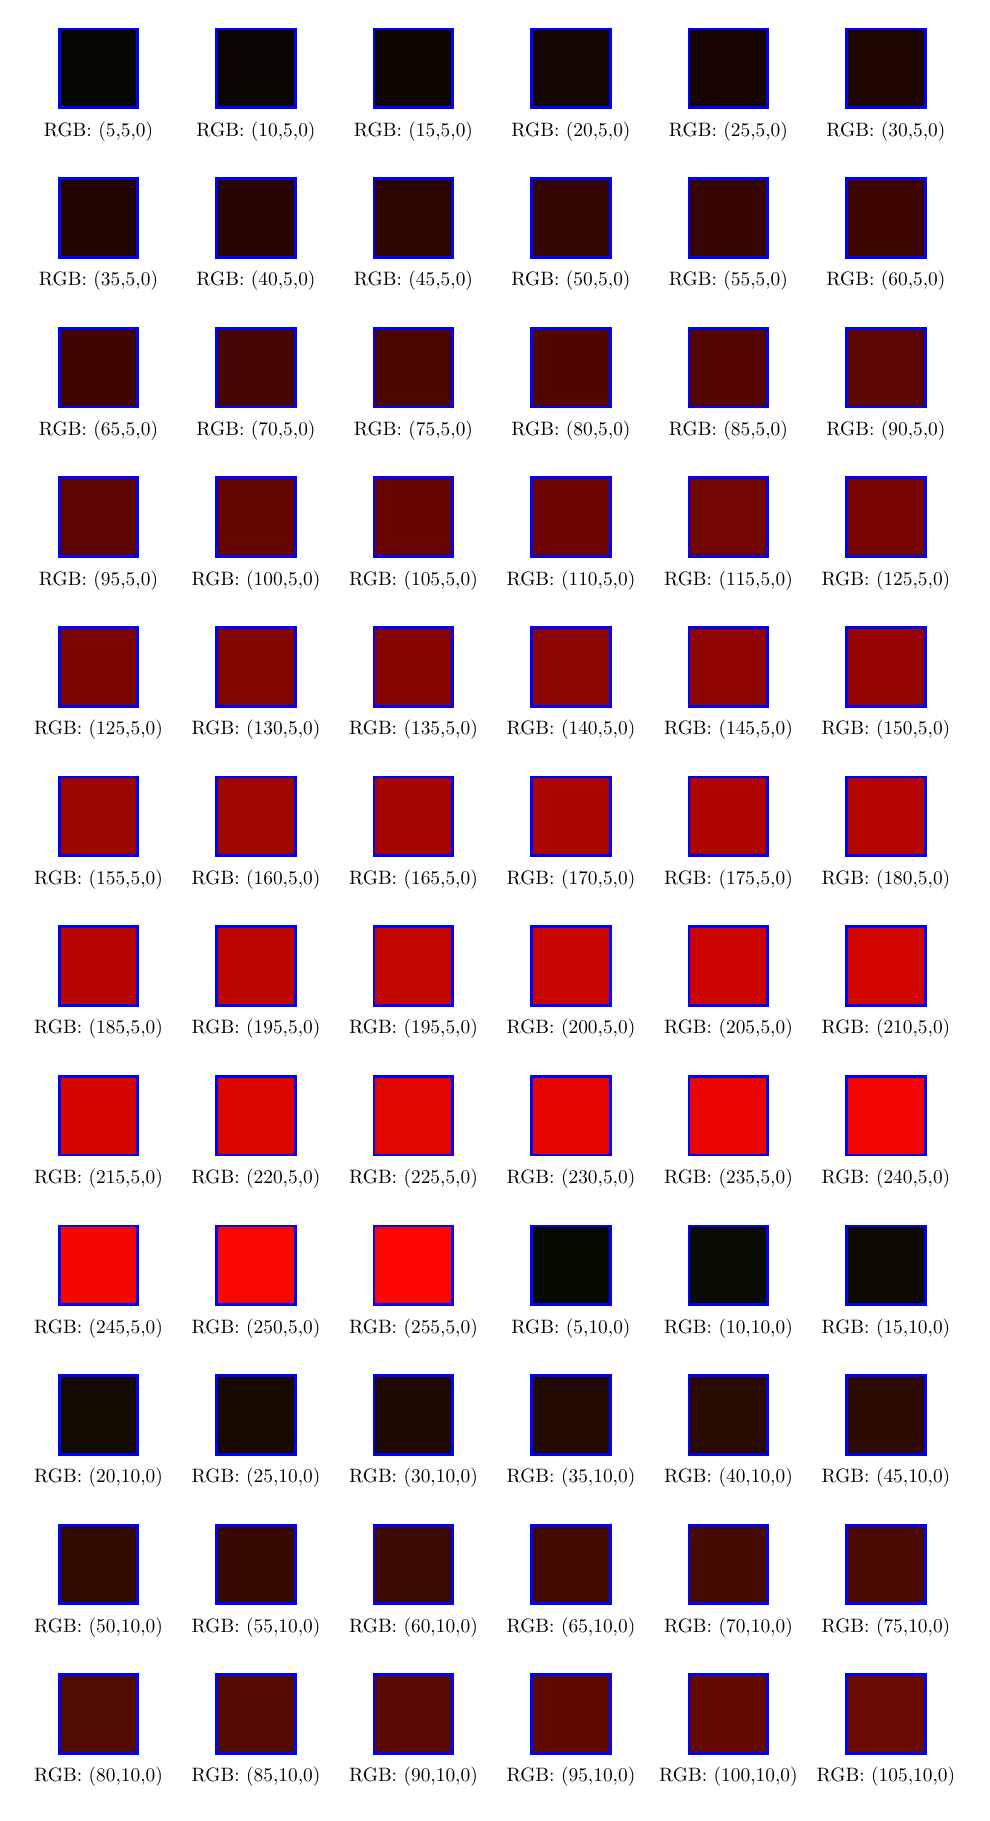
\begin{tikzpicture}

    \filldraw[draw=blue,line width=1,fill=colorR5G5B0]
    (0,0) rectangle (1,1);

    \node[scale=0.7] at (0.5,-0.3) {RGB: (5,5,0)};



    \begin{scope}[xshift=2cm]

      \filldraw[draw=blue,line width=1,fill=colorR10G5B0]
      (0,0) rectangle (1,1);

      \node[scale=0.7] at (0.5,-0.3) {RGB: (10,5,0)};

    \end{scope}



    \begin{scope}[xshift=4cm]

      \filldraw[draw=blue,line width=1,fill=colorR15G5B0]
      (0,0) rectangle (1,1);

      \node[scale=0.7] at (0.5,-0.3) {RGB: (15,5,0)};

    \end{scope}



    \begin{scope}[xshift=6cm]

      \filldraw[draw=blue,line width=1,fill=colorR20G5B0]
      (0,0) rectangle (1,1);

      \node[scale=0.7] at (0.5,-0.3) {RGB: (20,5,0)};

    \end{scope}



    \begin{scope}[xshift=8cm]

      \filldraw[draw=blue,line width=1,fill=colorR25G5B0]
      (0,0) rectangle (1,1);

      \node[scale=0.7] at (0.5,-0.3) {RGB: (25,5,0)};

    \end{scope}



    \begin{scope}[xshift=10cm]

      \filldraw[draw=blue,line width=1,fill=colorR30G5B0]
      (0,0) rectangle (1,1);

      \node[scale=0.7] at (0.5,-0.3) {RGB: (30,5,0)};

    \end{scope}







    \begin{scope}[yshift=-1.9cm]

      \filldraw[draw=blue,line width=1,fill=colorR35G5B0]
      (0,0) rectangle (1,1);

      \node[scale=0.7] at (0.5,-0.3) {RGB: (35,5,0)};

    \end{scope}



    \begin{scope}[xshift=2cm,yshift=-1.9cm]

      \filldraw[draw=blue,line width=1,fill=colorR40G5B0]
      (0,0) rectangle (1,1);

      \node[scale=0.7] at (0.5,-0.3) {RGB: (40,5,0)};

    \end{scope}



    \begin{scope}[xshift=4cm,yshift=-1.9cm]

      \filldraw[draw=blue,line width=1,fill=colorR45G5B0]
      (0,0) rectangle (1,1);

      \node[scale=0.7] at (0.5,-0.3) {RGB: (45,5,0)};

    \end{scope}



    \begin{scope}[xshift=6cm,yshift=-1.9cm]

      \filldraw[draw=blue,line width=1,fill=colorR50G5B0]
      (0,0) rectangle (1,1);

      \node[scale=0.7] at (0.5,-0.3) {RGB: (50,5,0)};

    \end{scope}



    \begin{scope}[xshift=8cm,yshift=-1.9cm]

      \filldraw[draw=blue,line width=1,fill=colorR55G5B0]
      (0,0) rectangle (1,1);

      \node[scale=0.7] at (0.5,-0.3) {RGB: (55,5,0)};

    \end{scope}



    \begin{scope}[xshift=10cm,yshift=-1.9cm]

      \filldraw[draw=blue,line width=1,fill=colorR60G5B0]
      (0,0) rectangle (1,1);

      \node[scale=0.7] at (0.5,-0.3) {RGB: (60,5,0)};

    \end{scope}







    \begin{scope}[yshift=-3.8cm]

      \filldraw[draw=blue,line width=1,fill=colorR65G5B0]
      (0,0) rectangle (1,1);

      \node[scale=0.7] at (0.5,-0.3) {RGB: (65,5,0)};

    \end{scope}



    \begin{scope}[xshift=2cm,yshift=-3.8cm]

      \filldraw[draw=blue,line width=1,fill=colorR70G5B0]
      (0,0) rectangle (1,1);

      \node[scale=0.7] at (0.5,-0.3) {RGB: (70,5,0)};

    \end{scope}



    \begin{scope}[xshift=4cm,yshift=-3.8cm]

      \filldraw[draw=blue,line width=1,fill=colorR75G5B0]
      (0,0) rectangle (1,1);

      \node[scale=0.7] at (0.5,-0.3) {RGB: (75,5,0)};

    \end{scope}



    \begin{scope}[xshift=6cm,yshift=-3.8cm]

      \filldraw[draw=blue,line width=1,fill=colorR80G5B0]
      (0,0) rectangle (1,1);

      \node[scale=0.7] at (0.5,-0.3) {RGB: (80,5,0)};

    \end{scope}



    \begin{scope}[xshift=8cm,yshift=-3.8cm]

      \filldraw[draw=blue,line width=1,fill=colorR85G5B0]
      (0,0) rectangle (1,1);

      \node[scale=0.7] at (0.5,-0.3) {RGB: (85,5,0)};

    \end{scope}



    \begin{scope}[xshift=10cm,yshift=-3.8cm]

      \filldraw[draw=blue,line width=1,fill=colorR90G5B0]
      (0,0) rectangle (1,1);

      \node[scale=0.7] at (0.5,-0.3) {RGB: (90,5,0)};

    \end{scope}







    \begin{scope}[yshift=-5.7cm]

      \filldraw[draw=blue,line width=1,fill=colorR95G5B0]
      (0,0) rectangle (1,1);

      \node[scale=0.7] at (0.5,-0.3) {RGB: (95,5,0)};

    \end{scope}



    \begin{scope}[xshift=2cm,yshift=-5.7cm]

      \filldraw[draw=blue,line width=1,fill=colorR100G5B0]
      (0,0) rectangle (1,1);

      \node[scale=0.7] at (0.5,-0.3) {RGB: (100,5,0)};

    \end{scope}



    \begin{scope}[xshift=4cm,yshift=-5.7cm]

      \filldraw[draw=blue,line width=1,fill=colorR105G5B0]
      (0,0) rectangle (1,1);

      \node[scale=0.7] at (0.5,-0.3) {RGB: (105,5,0)};

    \end{scope}



    \begin{scope}[xshift=6cm,yshift=-5.7cm]

      \filldraw[draw=blue,line width=1,fill=colorR110G5B0]
      (0,0) rectangle (1,1);

      \node[scale=0.7] at (0.5,-0.3) {RGB: (110,5,0)};

    \end{scope}



    \begin{scope}[xshift=8cm,yshift=-5.7cm]

      \filldraw[draw=blue,line width=1,fill=colorR115G5B0]
      (0,0) rectangle (1,1);

      \node[scale=0.7] at (0.5,-0.3) {RGB: (115,5,0)};

    \end{scope}



    \begin{scope}[xshift=10cm,yshift=-5.7cm]

      \filldraw[draw=blue,line width=1,fill=colorR120G5B0]
      (0,0) rectangle (1,1);

      \node[scale=0.7] at (0.5,-0.3) {RGB: (125,5,0)};

    \end{scope}







    \begin{scope}[yshift=-7.6cm]

      \filldraw[draw=blue,line width=1,fill=colorR125G5B0]
      (0,0) rectangle (1,1);

      \node[scale=0.7] at (0.5,-0.3) {RGB: (125,5,0)};

    \end{scope}



    \begin{scope}[xshift=2cm,yshift=-7.6cm]

      \filldraw[draw=blue,line width=1,fill=colorR130G5B0]
      (0,0) rectangle (1,1);

      \node[scale=0.7] at (0.5,-0.3) {RGB: (130,5,0)};

    \end{scope}



    \begin{scope}[xshift=4cm,yshift=-7.6cm]

      \filldraw[draw=blue,line width=1,fill=colorR135G5B0]
      (0,0) rectangle (1,1);

      \node[scale=0.7] at (0.5,-0.3) {RGB: (135,5,0)};

    \end{scope}



    \begin{scope}[xshift=6cm,yshift=-7.6cm]

      \filldraw[draw=blue,line width=1,fill=colorR140G5B0]
      (0,0) rectangle (1,1);

      \node[scale=0.7] at (0.5,-0.3) {RGB: (140,5,0)};

    \end{scope}



    \begin{scope}[xshift=8cm,yshift=-7.6cm]

      \filldraw[draw=blue,line width=1,fill=colorR145G5B0]
      (0,0) rectangle (1,1);

      \node[scale=0.7] at (0.5,-0.3) {RGB: (145,5,0)};

    \end{scope}



    \begin{scope}[xshift=10cm,yshift=-7.6cm]

      \filldraw[draw=blue,line width=1,fill=colorR150G5B0]
      (0,0) rectangle (1,1);

      \node[scale=0.7] at (0.5,-0.3) {RGB: (150,5,0)};

    \end{scope}







    \begin{scope}[yshift=-9.5cm]

      \filldraw[draw=blue,line width=1,fill=colorR155G5B0]
      (0,0) rectangle (1,1);

      \node[scale=0.7] at (0.5,-0.3) {RGB: (155,5,0)};

    \end{scope}



    \begin{scope}[xshift=2cm,yshift=-9.5cm]

      \filldraw[draw=blue,line width=1,fill=colorR160G5B0]
      (0,0) rectangle (1,1);

      \node[scale=0.7] at (0.5,-0.3) {RGB: (160,5,0)};

    \end{scope}



    \begin{scope}[xshift=4cm,yshift=-9.5cm]

      \filldraw[draw=blue,line width=1,fill=colorR165G5B0]
      (0,0) rectangle (1,1);

      \node[scale=0.7] at (0.5,-0.3) {RGB: (165,5,0)};

    \end{scope}



    \begin{scope}[xshift=6cm,yshift=-9.5cm]

      \filldraw[draw=blue,line width=1,fill=colorR170G5B0]
      (0,0) rectangle (1,1);

      \node[scale=0.7] at (0.5,-0.3) {RGB: (170,5,0)};

    \end{scope}



    \begin{scope}[xshift=8cm,yshift=-9.5cm]

      \filldraw[draw=blue,line width=1,fill=colorR175G5B0]
      (0,0) rectangle (1,1);

      \node[scale=0.7] at (0.5,-0.3) {RGB: (175,5,0)};

    \end{scope}



    \begin{scope}[xshift=10cm,yshift=-9.5cm]

      \filldraw[draw=blue,line width=1,fill=colorR180G5B0]
      (0,0) rectangle (1,1);

      \node[scale=0.7] at (0.5,-0.3) {RGB: (180,5,0)};

    \end{scope}







    \begin{scope}[yshift=-11.4cm]

      \filldraw[draw=blue,line width=1,fill=colorR185G5B0]
      (0,0) rectangle (1,1);

      \node[scale=0.7] at (0.5,-0.3) {RGB: (185,5,0)};

    \end{scope}



    \begin{scope}[xshift=2cm,yshift=-11.4cm]

      \filldraw[draw=blue,line width=1,fill=colorR190G5B0]
      (0,0) rectangle (1,1);

      \node[scale=0.7] at (0.5,-0.3) {RGB: (195,5,0)};

    \end{scope}



    \begin{scope}[xshift=4cm,yshift=-11.4cm]

      \filldraw[draw=blue,line width=1,fill=colorR195G5B0]
      (0,0) rectangle (1,1);

      \node[scale=0.7] at (0.5,-0.3) {RGB: (195,5,0)};

    \end{scope}



    \begin{scope}[xshift=6cm,yshift=-11.4cm]

      \filldraw[draw=blue,line width=1,fill=colorR200G5B0]
      (0,0) rectangle (1,1);

      \node[scale=0.7] at (0.5,-0.3) {RGB: (200,5,0)};

    \end{scope}



    \begin{scope}[xshift=8cm,yshift=-11.4cm]

      \filldraw[draw=blue,line width=1,fill=colorR205G5B0]
      (0,0) rectangle (1,1);

      \node[scale=0.7] at (0.5,-0.3) {RGB: (205,5,0)};

    \end{scope}



    \begin{scope}[xshift=10cm,yshift=-11.4cm]

      \filldraw[draw=blue,line width=1,fill=colorR210G5B0]
      (0,0) rectangle (1,1);

      \node[scale=0.7] at (0.5,-0.3) {RGB: (210,5,0)};

    \end{scope}







    \begin{scope}[yshift=-13.3cm]

      \filldraw[draw=blue,line width=1,fill=colorR215G5B0]
      (0,0) rectangle (1,1);

      \node[scale=0.7] at (0.5,-0.3) {RGB: (215,5,0)};

    \end{scope}



    \begin{scope}[xshift=2cm,yshift=-13.3cm]

      \filldraw[draw=blue,line width=1,fill=colorR220G5B0]
      (0,0) rectangle (1,1);

      \node[scale=0.7] at (0.5,-0.3) {RGB: (220,5,0)};

    \end{scope}



    \begin{scope}[xshift=4cm,yshift=-13.3cm]

      \filldraw[draw=blue,line width=1,fill=colorR225G5B0]
      (0,0) rectangle (1,1);

      \node[scale=0.7] at (0.5,-0.3) {RGB: (225,5,0)};

    \end{scope}



    \begin{scope}[xshift=6cm,yshift=-13.3cm]

      \filldraw[draw=blue,line width=1,fill=colorR230G5B0]
      (0,0) rectangle (1,1);

      \node[scale=0.7] at (0.5,-0.3) {RGB: (230,5,0)};

    \end{scope}



    \begin{scope}[xshift=8cm,yshift=-13.3cm]

      \filldraw[draw=blue,line width=1,fill=colorR235G5B0]
      (0,0) rectangle (1,1);

      \node[scale=0.7] at (0.5,-0.3) {RGB: (235,5,0)};

    \end{scope}



    \begin{scope}[xshift=10cm,yshift=-13.3cm]

      \filldraw[draw=blue,line width=1,fill=colorR240G5B0]
      (0,0) rectangle (1,1);

      \node[scale=0.7] at (0.5,-0.3) {RGB: (240,5,0)};

    \end{scope}







    \begin{scope}[yshift=-15.2cm]

      \filldraw[draw=blue,line width=1,fill=colorR245G5B0]
      (0,0) rectangle (1,1);

      \node[scale=0.7] at (0.5,-0.3) {RGB: (245,5,0)};

    \end{scope}



    \begin{scope}[xshift=2cm,yshift=-15.2cm]

      \filldraw[draw=blue,line width=1,fill=colorR250G5B0]
      (0,0) rectangle (1,1);

      \node[scale=0.7] at (0.5,-0.3) {RGB: (250,5,0)};

    \end{scope}



    \begin{scope}[xshift=4cm,yshift=-15.2cm]

      \filldraw[draw=blue,line width=1,fill=colorR255G5B0]
      (0,0) rectangle (1,1);

      \node[scale=0.7] at (0.5,-0.3) {RGB: (255,5,0)};

    \end{scope}



    \begin{scope}[xshift=6cm,yshift=-15.2cm]

      \filldraw[draw=blue,line width=1,fill=colorR5G10B0]
      (0,0) rectangle (1,1);

      \node[scale=0.7] at (0.5,-0.3) {RGB: (5,10,0)};

    \end{scope}



    \begin{scope}[xshift=8cm,yshift=-15.2cm]

      \filldraw[draw=blue,line width=1,fill=colorR10G10B0]
      (0,0) rectangle (1,1);

      \node[scale=0.7] at (0.5,-0.3) {RGB: (10,10,0)};

    \end{scope}



    \begin{scope}[xshift=10cm,yshift=-15.2cm]

      \filldraw[draw=blue,line width=1,fill=colorR15G10B0]
      (0,0) rectangle (1,1);

      \node[scale=0.7] at (0.5,-0.3) {RGB: (15,10,0)};

    \end{scope}







    \begin{scope}[yshift=-17.1cm]

      \filldraw[draw=blue,line width=1,fill=colorR20G10B0]
      (0,0) rectangle (1,1);

      \node[scale=0.7] at (0.5,-0.3) {RGB: (20,10,0)};

    \end{scope}



    \begin{scope}[xshift=2cm,yshift=-17.1cm]

      \filldraw[draw=blue,line width=1,fill=colorR25G10B0]
      (0,0) rectangle (1,1);

      \node[scale=0.7] at (0.5,-0.3) {RGB: (25,10,0)};

    \end{scope}



    \begin{scope}[xshift=4cm,yshift=-17.1cm]

      \filldraw[draw=blue,line width=1,fill=colorR30G10B0]
      (0,0) rectangle (1,1);

      \node[scale=0.7] at (0.5,-0.3) {RGB: (30,10,0)};

    \end{scope}



    \begin{scope}[xshift=6cm,yshift=-17.1cm]

      \filldraw[draw=blue,line width=1,fill=colorR35G10B0]
      (0,0) rectangle (1,1);

      \node[scale=0.7] at (0.5,-0.3) {RGB: (35,10,0)};

    \end{scope}



    \begin{scope}[xshift=8cm,yshift=-17.1cm]

      \filldraw[draw=blue,line width=1,fill=colorR40G10B0]
      (0,0) rectangle (1,1);

      \node[scale=0.7] at (0.5,-0.3) {RGB: (40,10,0)};

    \end{scope}



    \begin{scope}[xshift=10cm,yshift=-17.1cm]

      \filldraw[draw=blue,line width=1,fill=colorR45G10B0]
      (0,0) rectangle (1,1);

      \node[scale=0.7] at (0.5,-0.3) {RGB: (45,10,0)};

    \end{scope}







    \begin{scope}[yshift=-19cm]

      \filldraw[draw=blue,line width=1,fill=colorR50G10B0]
      (0,0) rectangle (1,1);

      \node[scale=0.7] at (0.5,-0.3) {RGB: (50,10,0)};

    \end{scope}



    \begin{scope}[xshift=2cm,yshift=-19cm]

      \filldraw[draw=blue,line width=1,fill=colorR55G10B0]
      (0,0) rectangle (1,1);

      \node[scale=0.7] at (0.5,-0.3) {RGB: (55,10,0)};

    \end{scope}



    \begin{scope}[xshift=4cm,yshift=-19cm]

      \filldraw[draw=blue,line width=1,fill=colorR60G10B0]
      (0,0) rectangle (1,1);

      \node[scale=0.7] at (0.5,-0.3) {RGB: (60,10,0)};

    \end{scope}



    \begin{scope}[xshift=6cm,yshift=-19cm]

      \filldraw[draw=blue,line width=1,fill=colorR65G10B0]
      (0,0) rectangle (1,1);

      \node[scale=0.7] at (0.5,-0.3) {RGB: (65,10,0)};

    \end{scope}



    \begin{scope}[xshift=8cm,yshift=-19cm]

      \filldraw[draw=blue,line width=1,fill=colorR70G10B0]
      (0,0) rectangle (1,1);

      \node[scale=0.7] at (0.5,-0.3) {RGB: (70,10,0)};

    \end{scope}



    \begin{scope}[xshift=10cm,yshift=-19cm]

      \filldraw[draw=blue,line width=1,fill=colorR75G10B0]
      (0,0) rectangle (1,1);

      \node[scale=0.7] at (0.5,-0.3) {RGB: (75,10,0)};

    \end{scope}







    \begin{scope}[yshift=-20.9cm]

      \filldraw[draw=blue,line width=1,fill=colorR80G10B0]
      (0,0) rectangle (1,1);

      \node[scale=0.7] at (0.5,-0.3) {RGB: (80,10,0)};

    \end{scope}



    \begin{scope}[xshift=2cm,yshift=-20.9cm]

      \filldraw[draw=blue,line width=1,fill=colorR85G10B0]
      (0,0) rectangle (1,1);

      \node[scale=0.7] at (0.5,-0.3) {RGB: (85,10,0)};

    \end{scope}



    \begin{scope}[xshift=4cm,yshift=-20.9cm]

      \filldraw[draw=blue,line width=1,fill=colorR90G10B0]
      (0,0) rectangle (1,1);

      \node[scale=0.7] at (0.5,-0.3) {RGB: (90,10,0)};

    \end{scope}



    \begin{scope}[xshift=6cm,yshift=-20.9cm]

      \filldraw[draw=blue,line width=1,fill=colorR95G10B0]
      (0,0) rectangle (1,1);

      \node[scale=0.7] at (0.5,-0.3) {RGB: (95,10,0)};

    \end{scope}



    \begin{scope}[xshift=8cm,yshift=-20.9cm]

      \filldraw[draw=blue,line width=1,fill=colorR100G10B0]
      (0,0) rectangle (1,1);

      \node[scale=0.7] at (0.5,-0.3) {RGB: (100,10,0)};

    \end{scope}



    \begin{scope}[xshift=10cm,yshift=-20.9cm]

      \filldraw[draw=blue,line width=1,fill=colorR105G10B0]
      (0,0) rectangle (1,1);

      \node[scale=0.7] at (0.5,-0.3) {RGB: (105,10,0)};

    \end{scope}

  \end{tikzpicture}

  \caption{Mixed colors in~RGB system: $(5,10,0)$--$(105,10,0)$}



  \label{fig:Mixed-colors-Part-01}

\end{figure}
% ##################





% ##################
\begin{figure}

  \centering


  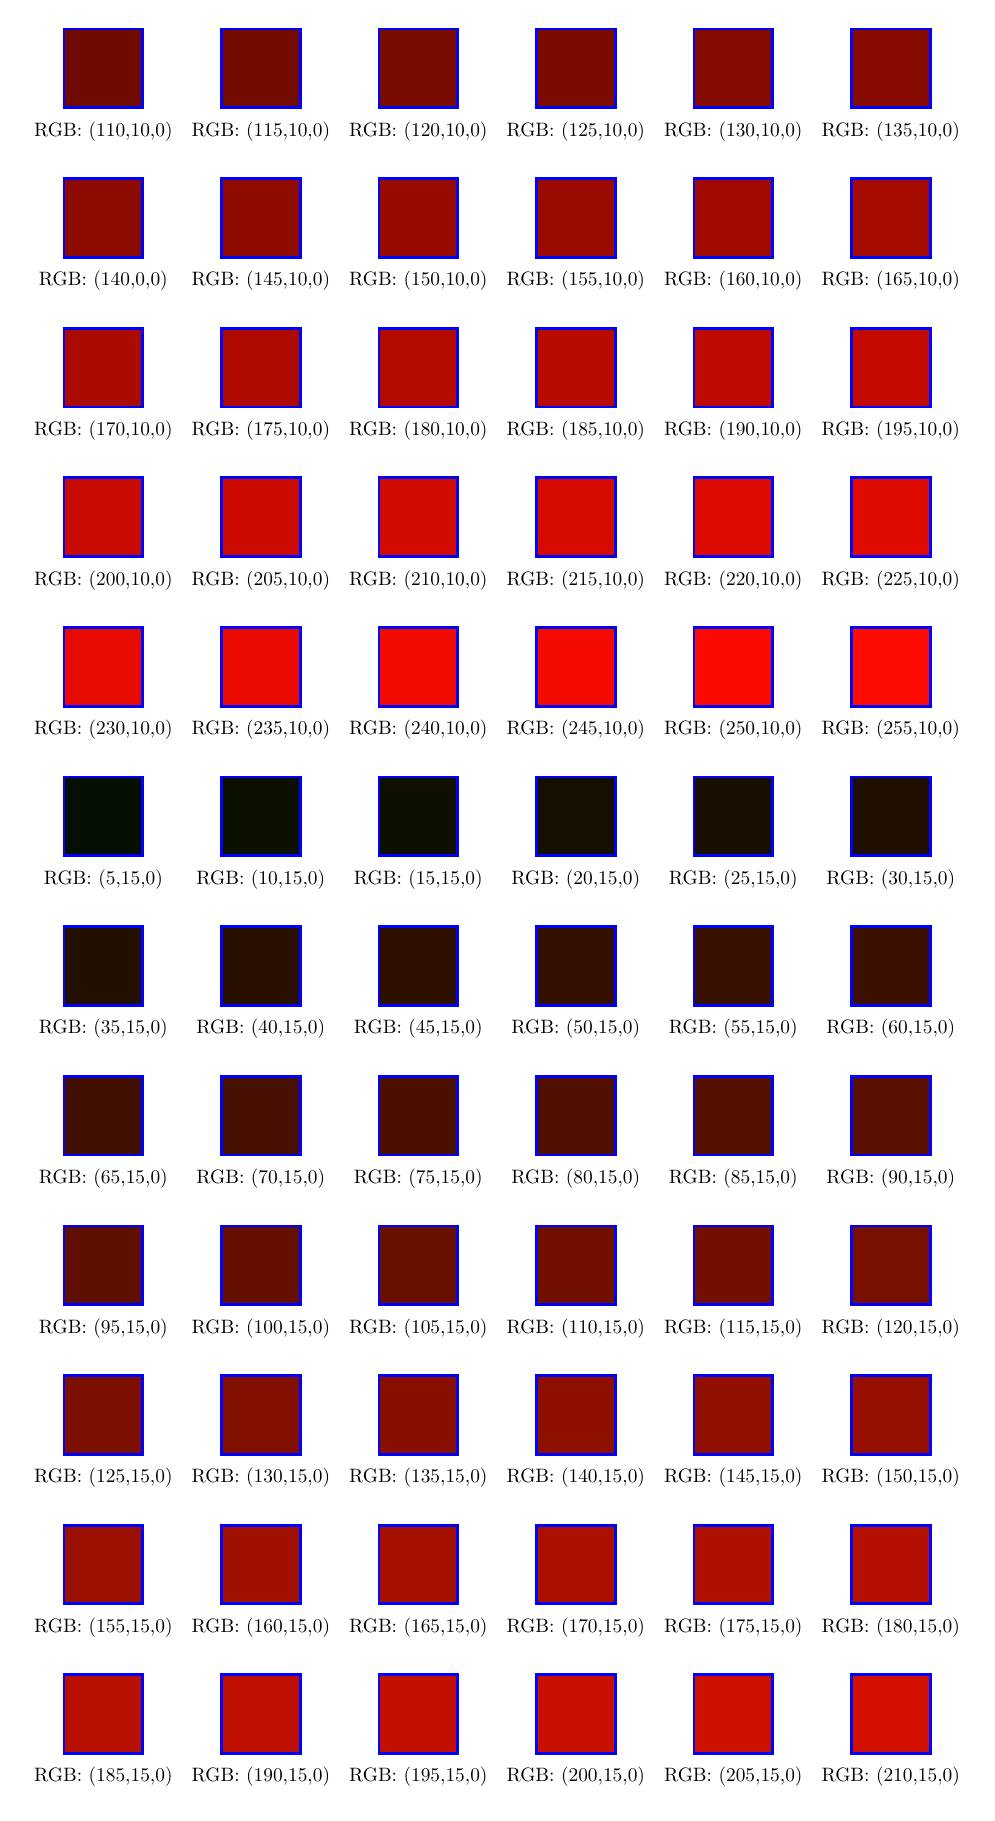
\begin{tikzpicture}

    \filldraw[draw=blue,line width=1,fill=colorR110G10B0]
    (0,0) rectangle (1,1);

    \node[scale=0.7] at (0.5,-0.3) {RGB: (110,10,0)};



    \begin{scope}[xshift=2cm]

      \filldraw[draw=blue,line width=1,fill=colorR115G10B0]
      (0,0) rectangle (1,1);

      \node[scale=0.7] at (0.5,-0.3) {RGB: (115,10,0)};

    \end{scope}



    \begin{scope}[xshift=4cm]

      \filldraw[draw=blue,line width=1,fill=colorR120G10B0]
      (0,0) rectangle (1,1);

      \node[scale=0.7] at (0.5,-0.3) {RGB: (120,10,0)};

    \end{scope}



    \begin{scope}[xshift=6cm]

      \filldraw[draw=blue,line width=1,fill=colorR125G10B0]
      (0,0) rectangle (1,1);

      \node[scale=0.7] at (0.5,-0.3) {RGB: (125,10,0)};

    \end{scope}



    \begin{scope}[xshift=8cm]

      \filldraw[draw=blue,line width=1,fill=colorR130G10B0]
      (0,0) rectangle (1,1);

      \node[scale=0.7] at (0.5,-0.3) {RGB: (130,10,0)};

    \end{scope}



    \begin{scope}[xshift=10cm]

      \filldraw[draw=blue,line width=1,fill=colorR135G10B0]
      (0,0) rectangle (1,1);

      \node[scale=0.7] at (0.5,-0.3) {RGB: (135,10,0)};

    \end{scope}







    \begin{scope}[yshift=-1.9cm]

      \filldraw[draw=blue,line width=1,fill=colorR140G10B0]
      (0,0) rectangle (1,1);

      \node[scale=0.7] at (0.5,-0.3) {RGB: (140,0,0)};

    \end{scope}



    \begin{scope}[xshift=2cm,yshift=-1.9cm]

      \filldraw[draw=blue,line width=1,fill=colorR145G10B0]
      (0,0) rectangle (1,1);

      \node[scale=0.7] at (0.5,-0.3) {RGB: (145,10,0)};

    \end{scope}



    \begin{scope}[xshift=4cm,yshift=-1.9cm]

      \filldraw[draw=blue,line width=1,fill=colorR150G10B0]
      (0,0) rectangle (1,1);

      \node[scale=0.7] at (0.5,-0.3) {RGB: (150,10,0)};

    \end{scope}



    \begin{scope}[xshift=6cm,yshift=-1.9cm]

      \filldraw[draw=blue,line width=1,fill=colorR155G10B0]
      (0,0) rectangle (1,1);

      \node[scale=0.7] at (0.5,-0.3) {RGB: (155,10,0)};

    \end{scope}



    \begin{scope}[xshift=8cm,yshift=-1.9cm]

      \filldraw[draw=blue,line width=1,fill=colorR160G10B0]
      (0,0) rectangle (1,1);

      \node[scale=0.7] at (0.5,-0.3) {RGB: (160,10,0)};

    \end{scope}



    \begin{scope}[xshift=10cm,yshift=-1.9cm]

      \filldraw[draw=blue,line width=1,fill=colorR165G10B0]
      (0,0) rectangle (1,1);

      \node[scale=0.7] at (0.5,-0.3) {RGB: (165,10,0)};

    \end{scope}







    \begin{scope}[yshift=-3.8cm]

      \filldraw[draw=blue,line width=1,fill=colorR170G10B0]
      (0,0) rectangle (1,1);

      \node[scale=0.7] at (0.5,-0.3) {RGB: (170,10,0)};

    \end{scope}



    \begin{scope}[xshift=2cm,yshift=-3.8cm]

      \filldraw[draw=blue,line width=1,fill=colorR175G10B0]
      (0,0) rectangle (1,1);

      \node[scale=0.7] at (0.5,-0.3) {RGB: (175,10,0)};

    \end{scope}



    \begin{scope}[xshift=4cm,yshift=-3.8cm]

      \filldraw[draw=blue,line width=1,fill=colorR180G10B0]
      (0,0) rectangle (1,1);

      \node[scale=0.7] at (0.5,-0.3) {RGB: (180,10,0)};

    \end{scope}



    \begin{scope}[xshift=6cm,yshift=-3.8cm]

      \filldraw[draw=blue,line width=1,fill=colorR185G10B0]
      (0,0) rectangle (1,1);

      \node[scale=0.7] at (0.5,-0.3) {RGB: (185,10,0)};

    \end{scope}



    \begin{scope}[xshift=8cm,yshift=-3.8cm]

      \filldraw[draw=blue,line width=1,fill=colorR190G10B0]
      (0,0) rectangle (1,1);

      \node[scale=0.7] at (0.5,-0.3) {RGB: (190,10,0)};

    \end{scope}



    \begin{scope}[xshift=10cm,yshift=-3.8cm]

      \filldraw[draw=blue,line width=1,fill=colorR195G10B0]
      (0,0) rectangle (1,1);

      \node[scale=0.7] at (0.5,-0.3) {RGB: (195,10,0)};

    \end{scope}







    \begin{scope}[yshift=-5.7cm]

      \filldraw[draw=blue,line width=1,fill=colorR200G10B0]
      (0,0) rectangle (1,1);

      \node[scale=0.7] at (0.5,-0.3) {RGB: (200,10,0)};

    \end{scope}



    \begin{scope}[xshift=2cm,yshift=-5.7cm]

      \filldraw[draw=blue,line width=1,fill=colorR205G10B0]
      (0,0) rectangle (1,1);

      \node[scale=0.7] at (0.5,-0.3) {RGB: (205,10,0)};

    \end{scope}



    \begin{scope}[xshift=4cm,yshift=-5.7cm]

      \filldraw[draw=blue,line width=1,fill=colorR210G10B0]
      (0,0) rectangle (1,1);

      \node[scale=0.7] at (0.5,-0.3) {RGB: (210,10,0)};

    \end{scope}



    \begin{scope}[xshift=6cm,yshift=-5.7cm]

      \filldraw[draw=blue,line width=1,fill=colorR215G10B0]
      (0,0) rectangle (1,1);

      \node[scale=0.7] at (0.5,-0.3) {RGB: (215,10,0)};

    \end{scope}



    \begin{scope}[xshift=8cm,yshift=-5.7cm]

      \filldraw[draw=blue,line width=1,fill=colorR220G10B0]
      (0,0) rectangle (1,1);

      \node[scale=0.7] at (0.5,-0.3) {RGB: (220,10,0)};

    \end{scope}



    \begin{scope}[xshift=10cm,yshift=-5.7cm]

      \filldraw[draw=blue,line width=1,fill=colorR225G10B0]
      (0,0) rectangle (1,1);

      \node[scale=0.7] at (0.5,-0.3) {RGB: (225,10,0)};

    \end{scope}







    \begin{scope}[yshift=-7.6cm]

      \filldraw[draw=blue,line width=1,fill=colorR230G10B0]
      (0,0) rectangle (1,1);

      \node[scale=0.7] at (0.5,-0.3) {RGB: (230,10,0)};

    \end{scope}



    \begin{scope}[xshift=2cm,yshift=-7.6cm]

      \filldraw[draw=blue,line width=1,fill=colorR235G10B0]
      (0,0) rectangle (1,1);

      \node[scale=0.7] at (0.5,-0.3) {RGB: (235,10,0)};

    \end{scope}



    \begin{scope}[xshift=4cm,yshift=-7.6cm]

      \filldraw[draw=blue,line width=1,fill=colorR240G10B0]
      (0,0) rectangle (1,1);

      \node[scale=0.7] at (0.5,-0.3) {RGB: (240,10,0)};

    \end{scope}



    \begin{scope}[xshift=6cm,yshift=-7.6cm]

      \filldraw[draw=blue,line width=1,fill=colorR245G10B0]
      (0,0) rectangle (1,1);

      \node[scale=0.7] at (0.5,-0.3) {RGB: (245,10,0)};

    \end{scope}



    \begin{scope}[xshift=8cm,yshift=-7.6cm]

      \filldraw[draw=blue,line width=1,fill=colorR250G10B0]
      (0,0) rectangle (1,1);

      \node[scale=0.7] at (0.5,-0.3) {RGB: (250,10,0)};

    \end{scope}



    \begin{scope}[xshift=10cm,yshift=-7.6cm]

      \filldraw[draw=blue,line width=1,fill=colorR255G10B0]
      (0,0) rectangle (1,1);

      \node[scale=0.7] at (0.5,-0.3) {RGB: (255,10,0)};

    \end{scope}







    \begin{scope}[yshift=-9.5cm]

      \filldraw[draw=blue,line width=1,fill=colorR5G15B0]
      (0,0) rectangle (1,1);

      \node[scale=0.7] at (0.5,-0.3) {RGB: (5,15,0)};

    \end{scope}



    \begin{scope}[xshift=2cm,yshift=-9.5cm]

      \filldraw[draw=blue,line width=1,fill=colorR10G15B0]
      (0,0) rectangle (1,1);

      \node[scale=0.7] at (0.5,-0.3) {RGB: (10,15,0)};

    \end{scope}



    \begin{scope}[xshift=4cm,yshift=-9.5cm]

      \filldraw[draw=blue,line width=1,fill=colorR15G15B0]
      (0,0) rectangle (1,1);

      \node[scale=0.7] at (0.5,-0.3) {RGB: (15,15,0)};

    \end{scope}



    \begin{scope}[xshift=6cm,yshift=-9.5cm]

      \filldraw[draw=blue,line width=1,fill=colorR20G15B0]
      (0,0) rectangle (1,1);

      \node[scale=0.7] at (0.5,-0.3) {RGB: (20,15,0)};

    \end{scope}



    \begin{scope}[xshift=8cm,yshift=-9.5cm]

      \filldraw[draw=blue,line width=1,fill=colorR25G15B0]
      (0,0) rectangle (1,1);

      \node[scale=0.7] at (0.5,-0.3) {RGB: (25,15,0)};

    \end{scope}



    \begin{scope}[xshift=10cm,yshift=-9.5cm]

      \filldraw[draw=blue,line width=1,fill=colorR30G15B0]
      (0,0) rectangle (1,1);

      \node[scale=0.7] at (0.5,-0.3) {RGB: (30,15,0)};

    \end{scope}







    \begin{scope}[yshift=-11.4cm]

      \filldraw[draw=blue,line width=1,fill=colorR35G15B0]
      (0,0) rectangle (1,1);

      \node[scale=0.7] at (0.5,-0.3) {RGB: (35,15,0)};

    \end{scope}



    \begin{scope}[xshift=2cm,yshift=-11.4cm]

      \filldraw[draw=blue,line width=1,fill=colorR40G15B0]
      (0,0) rectangle (1,1);

      \node[scale=0.7] at (0.5,-0.3) {RGB: (40,15,0)};

    \end{scope}



    \begin{scope}[xshift=4cm,yshift=-11.4cm]

      \filldraw[draw=blue,line width=1,fill=colorR45G15B0]
      (0,0) rectangle (1,1);

      \node[scale=0.7] at (0.5,-0.3) {RGB: (45,15,0)};

    \end{scope}



    \begin{scope}[xshift=6cm,yshift=-11.4cm]

      \filldraw[draw=blue,line width=1,fill=colorR50G15B0]
      (0,0) rectangle (1,1);

      \node[scale=0.7] at (0.5,-0.3) {RGB: (50,15,0)};

    \end{scope}



    \begin{scope}[xshift=8cm,yshift=-11.4cm]

      \filldraw[draw=blue,line width=1,fill=colorR55G15B0]
      (0,0) rectangle (1,1);

      \node[scale=0.7] at (0.5,-0.3) {RGB: (55,15,0)};

    \end{scope}



    \begin{scope}[xshift=10cm,yshift=-11.4cm]

      \filldraw[draw=blue,line width=1,fill=colorR60G15B0]
      (0,0) rectangle (1,1);

      \node[scale=0.7] at (0.5,-0.3) {RGB: (60,15,0)};

    \end{scope}







    \begin{scope}[yshift=-13.3cm]

      \filldraw[draw=blue,line width=1,fill=colorR65G15B0]
      (0,0) rectangle (1,1);

      \node[scale=0.7] at (0.5,-0.3) {RGB: (65,15,0)};

    \end{scope}



    \begin{scope}[xshift=2cm,yshift=-13.3cm]

      \filldraw[draw=blue,line width=1,fill=colorR70G15B0]
      (0,0) rectangle (1,1);

      \node[scale=0.7] at (0.5,-0.3) {RGB: (70,15,0)};

    \end{scope}



    \begin{scope}[xshift=4cm,yshift=-13.3cm]

      \filldraw[draw=blue,line width=1,fill=colorR75G15B0]
      (0,0) rectangle (1,1);

      \node[scale=0.7] at (0.5,-0.3) {RGB: (75,15,0)};

    \end{scope}



    \begin{scope}[xshift=6cm,yshift=-13.3cm]

      \filldraw[draw=blue,line width=1,fill=colorR80G15B0]
      (0,0) rectangle (1,1);

      \node[scale=0.7] at (0.5,-0.3) {RGB: (80,15,0)};

    \end{scope}



    \begin{scope}[xshift=8cm,yshift=-13.3cm]

      \filldraw[draw=blue,line width=1,fill=colorR85G15B0]
      (0,0) rectangle (1,1);

      \node[scale=0.7] at (0.5,-0.3) {RGB: (85,15,0)};

    \end{scope}



    \begin{scope}[xshift=10cm,yshift=-13.3cm]

      \filldraw[draw=blue,line width=1,fill=colorR90G15B0]
      (0,0) rectangle (1,1);

      \node[scale=0.7] at (0.5,-0.3) {RGB: (90,15,0)};

    \end{scope}







    \begin{scope}[yshift=-15.2cm]

      \filldraw[draw=blue,line width=1,fill=colorR95G15B0]
      (0,0) rectangle (1,1);

      \node[scale=0.7] at (0.5,-0.3) {RGB: (95,15,0)};

    \end{scope}



    \begin{scope}[xshift=2cm,yshift=-15.2cm]

      \filldraw[draw=blue,line width=1,fill=colorR100G15B0]
      (0,0) rectangle (1,1);

      \node[scale=0.7] at (0.5,-0.3) {RGB: (100,15,0)};

    \end{scope}



    \begin{scope}[xshift=4cm,yshift=-15.2cm]

      \filldraw[draw=blue,line width=1,fill=colorR105G15B0]
      (0,0) rectangle (1,1);

      \node[scale=0.7] at (0.5,-0.3) {RGB: (105,15,0)};

    \end{scope}



    \begin{scope}[xshift=6cm,yshift=-15.2cm]

      \filldraw[draw=blue,line width=1,fill=colorR110G15B0]
      (0,0) rectangle (1,1);

      \node[scale=0.7] at (0.5,-0.3) {RGB: (110,15,0)};

    \end{scope}



    \begin{scope}[xshift=8cm,yshift=-15.2cm]

      \filldraw[draw=blue,line width=1,fill=colorR115G15B0]
      (0,0) rectangle (1,1);

      \node[scale=0.7] at (0.5,-0.3) {RGB: (115,15,0)};

    \end{scope}



    \begin{scope}[xshift=10cm,yshift=-15.2cm]

      \filldraw[draw=blue,line width=1,fill=colorR120G15B0]
      (0,0) rectangle (1,1);

      \node[scale=0.7] at (0.5,-0.3) {RGB: (120,15,0)};

    \end{scope}







    \begin{scope}[yshift=-17.1cm]

      \filldraw[draw=blue,line width=1,fill=colorR125G15B0]
      (0,0) rectangle (1,1);

      \node[scale=0.7] at (0.5,-0.3) {RGB: (125,15,0)};

    \end{scope}



    \begin{scope}[xshift=2cm,yshift=-17.1cm]

      \filldraw[draw=blue,line width=1,fill=colorR130G15B0]
      (0,0) rectangle (1,1);

      \node[scale=0.7] at (0.5,-0.3) {RGB: (130,15,0)};

    \end{scope}



    \begin{scope}[xshift=4cm,yshift=-17.1cm]

      \filldraw[draw=blue,line width=1,fill=colorR135G15B0]
      (0,0) rectangle (1,1);

      \node[scale=0.7] at (0.5,-0.3) {RGB: (135,15,0)};

    \end{scope}



    \begin{scope}[xshift=6cm,yshift=-17.1cm]

      \filldraw[draw=blue,line width=1,fill=colorR140G15B0]
      (0,0) rectangle (1,1);

      \node[scale=0.7] at (0.5,-0.3) {RGB: (140,15,0)};

    \end{scope}



    \begin{scope}[xshift=8cm,yshift=-17.1cm]

      \filldraw[draw=blue,line width=1,fill=colorR145G15B0]
      (0,0) rectangle (1,1);

      \node[scale=0.7] at (0.5,-0.3) {RGB: (145,15,0)};

    \end{scope}



    \begin{scope}[xshift=10cm,yshift=-17.1cm]

      \filldraw[draw=blue,line width=1,fill=colorR150G15B0]
      (0,0) rectangle (1,1);

      \node[scale=0.7] at (0.5,-0.3) {RGB: (150,15,0)};

    \end{scope}







    \begin{scope}[yshift=-19cm]

      \filldraw[draw=blue,line width=1,fill=colorR155G15B0]
      (0,0) rectangle (1,1);

      \node[scale=0.7] at (0.5,-0.3) {RGB: (155,15,0)};

    \end{scope}



    \begin{scope}[xshift=2cm,yshift=-19cm]

      \filldraw[draw=blue,line width=1,fill=colorR160G15B0]
      (0,0) rectangle (1,1);

      \node[scale=0.7] at (0.5,-0.3) {RGB: (160,15,0)};

    \end{scope}



    \begin{scope}[xshift=4cm,yshift=-19cm]

      \filldraw[draw=blue,line width=1,fill=colorR165G15B0]
      (0,0) rectangle (1,1);

      \node[scale=0.7] at (0.5,-0.3) {RGB: (165,15,0)};

    \end{scope}



    \begin{scope}[xshift=6cm,yshift=-19cm]

      \filldraw[draw=blue,line width=1,fill=colorR170G15B0]
      (0,0) rectangle (1,1);

      \node[scale=0.7] at (0.5,-0.3) {RGB: (170,15,0)};

    \end{scope}



    \begin{scope}[xshift=8cm,yshift=-19cm]

      \filldraw[draw=blue,line width=1,fill=colorR175G15B0]
      (0,0) rectangle (1,1);

      \node[scale=0.7] at (0.5,-0.3) {RGB: (175,15,0)};

    \end{scope}



    \begin{scope}[xshift=10cm,yshift=-19cm]

      \filldraw[draw=blue,line width=1,fill=colorR180G15B0]
      (0,0) rectangle (1,1);

      \node[scale=0.7] at (0.5,-0.3) {RGB: (180,15,0)};

    \end{scope}







    \begin{scope}[yshift=-20.9cm]

      \filldraw[draw=blue,line width=1,fill=colorR185G15B0]
      (0,0) rectangle (1,1);

      \node[scale=0.7] at (0.5,-0.3) {RGB: (185,15,0)};

    \end{scope}



    \begin{scope}[xshift=2cm,yshift=-20.9cm]

      \filldraw[draw=blue,line width=1,fill=colorR190G15B0]
      (0,0) rectangle (1,1);

      \node[scale=0.7] at (0.5,-0.3) {RGB: (190,15,0)};

    \end{scope}



    \begin{scope}[xshift=4cm,yshift=-20.9cm]

      \filldraw[draw=blue,line width=1,fill=colorR195G15B0]
      (0,0) rectangle (1,1);

      \node[scale=0.7] at (0.5,-0.3) {RGB: (195,15,0)};

    \end{scope}



    \begin{scope}[xshift=6cm,yshift=-20.9cm]

      \filldraw[draw=blue,line width=1,fill=colorR200G15B0]
      (0,0) rectangle (1,1);

      \node[scale=0.7] at (0.5,-0.3) {RGB: (200,15,0)};

    \end{scope}



    \begin{scope}[xshift=8cm,yshift=-20.9cm]

      \filldraw[draw=blue,line width=1,fill=colorR205G15B0]
      (0,0) rectangle (1,1);

      \node[scale=0.7] at (0.5,-0.3) {RGB: (205,15,0)};

    \end{scope}



    \begin{scope}[xshift=10cm,yshift=-20.9cm]

      \filldraw[draw=blue,line width=1,fill=colorR210G15B0]
      (0,0) rectangle (1,1);

      \node[scale=0.7] at (0.5,-0.3) {RGB: (210,15,0)};

    \end{scope}

  \end{tikzpicture}

  \caption{Mixed colors in~RGB system: $(110,10,0)$--$(255,10,0)$,
    $(5,15,0)$--$(210,15,0)$}



  \label{fig:Mixed-colors-Part-02}

\end{figure}
% ##################





% ##################
\begin{figure}

  \centering


  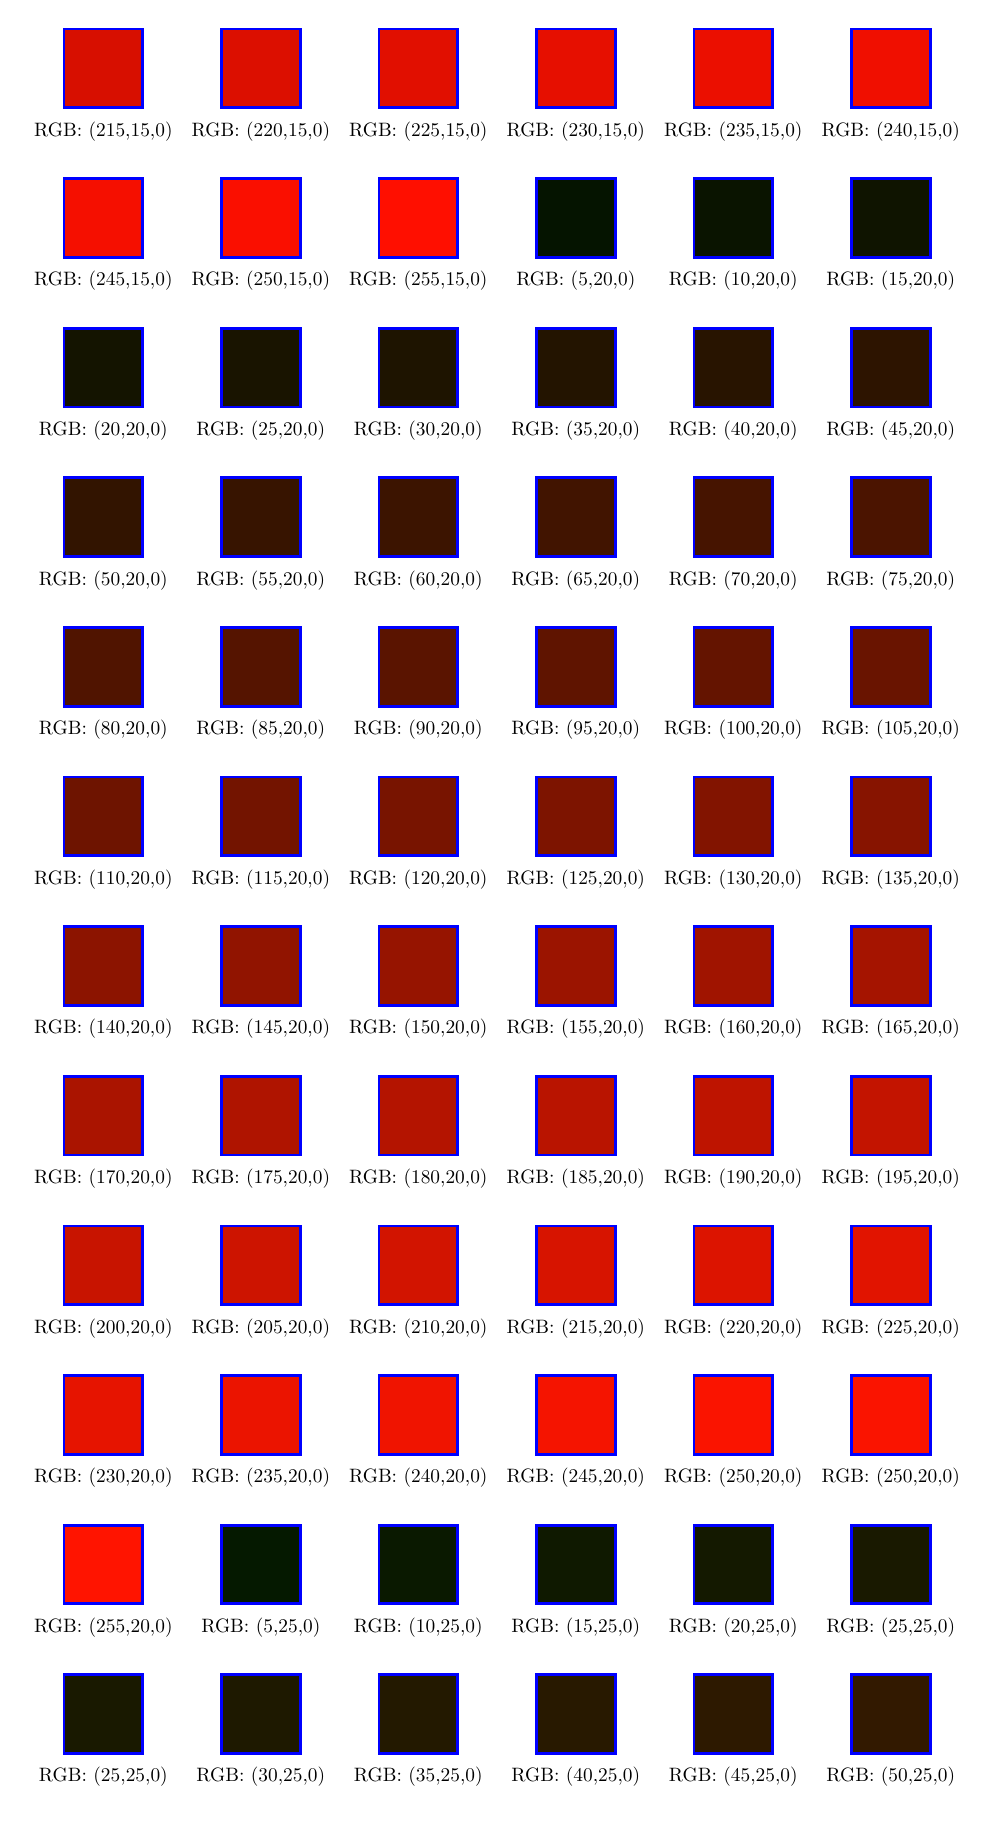
\begin{tikzpicture}

    \filldraw[draw=blue,line width=1,fill=colorR215G15B0]
    (0,0) rectangle (1,1);

    \node[scale=0.7] at (0.5,-0.3) {RGB: (215,15,0)};



    \begin{scope}[xshift=2cm]

      \filldraw[draw=blue,line width=1,fill=colorR220G15B0]
      (0,0) rectangle (1,1);

      \node[scale=0.7] at (0.5,-0.3) {RGB: (220,15,0)};

    \end{scope}



    \begin{scope}[xshift=4cm]

      \filldraw[draw=blue,line width=1,fill=colorR225G15B0]
      (0,0) rectangle (1,1);

      \node[scale=0.7] at (0.5,-0.3) {RGB: (225,15,0)};

    \end{scope}



    \begin{scope}[xshift=6cm]

      \filldraw[draw=blue,line width=1,fill=colorR230G15B0]
      (0,0) rectangle (1,1);

      \node[scale=0.7] at (0.5,-0.3) {RGB: (230,15,0)};

    \end{scope}



    \begin{scope}[xshift=8cm]

      \filldraw[draw=blue,line width=1,fill=colorR235G15B0]
      (0,0) rectangle (1,1);

      \node[scale=0.7] at (0.5,-0.3) {RGB: (235,15,0)};

    \end{scope}



    \begin{scope}[xshift=10cm]

      \filldraw[draw=blue,line width=1,fill=colorR240G15B0]
      (0,0) rectangle (1,1);

      \node[scale=0.7] at (0.5,-0.3) {RGB: (240,15,0)};

    \end{scope}







    \begin{scope}[yshift=-1.9cm]

      \filldraw[draw=blue,line width=1,fill=colorR245G15B0]
      (0,0) rectangle (1,1);

      \node[scale=0.7] at (0.5,-0.3) {RGB: (245,15,0)};

    \end{scope}



    \begin{scope}[xshift=2cm,yshift=-1.9cm]

      \filldraw[draw=blue,line width=1,fill=colorR250G15B0]
      (0,0) rectangle (1,1);

      \node[scale=0.7] at (0.5,-0.3) {RGB: (250,15,0)};

    \end{scope}



    \begin{scope}[xshift=4cm,yshift=-1.9cm]

      \filldraw[draw=blue,line width=1,fill=colorR255G15B0]
      (0,0) rectangle (1,1);

      \node[scale=0.7] at (0.5,-0.3) {RGB: (255,15,0)};

    \end{scope}



    \begin{scope}[xshift=6cm,yshift=-1.9cm]

      \filldraw[draw=blue,line width=1,fill=colorR5G20B0]
      (0,0) rectangle (1,1);

      \node[scale=0.7] at (0.5,-0.3) {RGB: (5,20,0)};

    \end{scope}



    \begin{scope}[xshift=8cm,yshift=-1.9cm]

      \filldraw[draw=blue,line width=1,fill=colorR10G20B0]
      (0,0) rectangle (1,1);

      \node[scale=0.7] at (0.5,-0.3) {RGB: (10,20,0)};

    \end{scope}



    \begin{scope}[xshift=10cm,yshift=-1.9cm]

      \filldraw[draw=blue,line width=1,fill=colorR15G20B0]
      (0,0) rectangle (1,1);

      \node[scale=0.7] at (0.5,-0.3) {RGB: (15,20,0)};

    \end{scope}







    \begin{scope}[yshift=-3.8cm]

      \filldraw[draw=blue,line width=1,fill=colorR20G20B0]
      (0,0) rectangle (1,1);

      \node[scale=0.7] at (0.5,-0.3) {RGB: (20,20,0)};

    \end{scope}



    \begin{scope}[xshift=2cm,yshift=-3.8cm]

      \filldraw[draw=blue,line width=1,fill=colorR25G20B0]
      (0,0) rectangle (1,1);

      \node[scale=0.7] at (0.5,-0.3) {RGB: (25,20,0)};

    \end{scope}



    \begin{scope}[xshift=4cm,yshift=-3.8cm]

      \filldraw[draw=blue,line width=1,fill=colorR30G20B0]
      (0,0) rectangle (1,1);

      \node[scale=0.7] at (0.5,-0.3) {RGB: (30,20,0)};

    \end{scope}



    \begin{scope}[xshift=6cm,yshift=-3.8cm]

      \filldraw[draw=blue,line width=1,fill=colorR35G20B0]
      (0,0) rectangle (1,1);

      \node[scale=0.7] at (0.5,-0.3) {RGB: (35,20,0)};

    \end{scope}



    \begin{scope}[xshift=8cm,yshift=-3.8cm]

      \filldraw[draw=blue,line width=1,fill=colorR40G20B0]
      (0,0) rectangle (1,1);

      \node[scale=0.7] at (0.5,-0.3) {RGB: (40,20,0)};

    \end{scope}



    \begin{scope}[xshift=10cm,yshift=-3.8cm]

      \filldraw[draw=blue,line width=1,fill=colorR45G20B0]
      (0,0) rectangle (1,1);

      \node[scale=0.7] at (0.5,-0.3) {RGB: (45,20,0)};

    \end{scope}







    \begin{scope}[yshift=-5.7cm]

      \filldraw[draw=blue,line width=1,fill=colorR50G20B0]
      (0,0) rectangle (1,1);

      \node[scale=0.7] at (0.5,-0.3) {RGB: (50,20,0)};

    \end{scope}



    \begin{scope}[xshift=2cm,yshift=-5.7cm]

      \filldraw[draw=blue,line width=1,fill=colorR55G20B0]
      (0,0) rectangle (1,1);

      \node[scale=0.7] at (0.5,-0.3) {RGB: (55,20,0)};

    \end{scope}



    \begin{scope}[xshift=4cm,yshift=-5.7cm]

      \filldraw[draw=blue,line width=1,fill=colorR60G20B0]
      (0,0) rectangle (1,1);

      \node[scale=0.7] at (0.5,-0.3) {RGB: (60,20,0)};

    \end{scope}



    \begin{scope}[xshift=6cm,yshift=-5.7cm]

      \filldraw[draw=blue,line width=1,fill=colorR65G20B0]
      (0,0) rectangle (1,1);

      \node[scale=0.7] at (0.5,-0.3) {RGB: (65,20,0)};

    \end{scope}



    \begin{scope}[xshift=8cm,yshift=-5.7cm]

      \filldraw[draw=blue,line width=1,fill=colorR70G20B0]
      (0,0) rectangle (1,1);

      \node[scale=0.7] at (0.5,-0.3) {RGB: (70,20,0)};

    \end{scope}



    \begin{scope}[xshift=10cm,yshift=-5.7cm]

      \filldraw[draw=blue,line width=1,fill=colorR75G20B0]
      (0,0) rectangle (1,1);

      \node[scale=0.7] at (0.5,-0.3) {RGB: (75,20,0)};

    \end{scope}







    \begin{scope}[yshift=-7.6cm]

      \filldraw[draw=blue,line width=1,fill=colorR80G20B0]
      (0,0) rectangle (1,1);

      \node[scale=0.7] at (0.5,-0.3) {RGB: (80,20,0)};

    \end{scope}



    \begin{scope}[xshift=2cm,yshift=-7.6cm]

      \filldraw[draw=blue,line width=1,fill=colorR85G20B0]
      (0,0) rectangle (1,1);

      \node[scale=0.7] at (0.5,-0.3) {RGB: (85,20,0)};

    \end{scope}



    \begin{scope}[xshift=4cm,yshift=-7.6cm]

      \filldraw[draw=blue,line width=1,fill=colorR90G20B0]
      (0,0) rectangle (1,1);

      \node[scale=0.7] at (0.5,-0.3) {RGB: (90,20,0)};

    \end{scope}



    \begin{scope}[xshift=6cm,yshift=-7.6cm]

      \filldraw[draw=blue,line width=1,fill=colorR95G20B0]
      (0,0) rectangle (1,1);

      \node[scale=0.7] at (0.5,-0.3) {RGB: (95,20,0)};

    \end{scope}



    \begin{scope}[xshift=8cm,yshift=-7.6cm]

      \filldraw[draw=blue,line width=1,fill=colorR100G20B0]
      (0,0) rectangle (1,1);

      \node[scale=0.7] at (0.5,-0.3) {RGB: (100,20,0)};

    \end{scope}



    \begin{scope}[xshift=10cm,yshift=-7.6cm]

      \filldraw[draw=blue,line width=1,fill=colorR105G20B0]
      (0,0) rectangle (1,1);

      \node[scale=0.7] at (0.5,-0.3) {RGB: (105,20,0)};

    \end{scope}







    \begin{scope}[yshift=-9.5cm]

      \filldraw[draw=blue,line width=1,fill=colorR110G20B0]
      (0,0) rectangle (1,1);

      \node[scale=0.7] at (0.5,-0.3) {RGB: (110,20,0)};

    \end{scope}



    \begin{scope}[xshift=2cm,yshift=-9.5cm]

      \filldraw[draw=blue,line width=1,fill=colorR115G20B0]
      (0,0) rectangle (1,1);

      \node[scale=0.7] at (0.5,-0.3) {RGB: (115,20,0)};

    \end{scope}



    \begin{scope}[xshift=4cm,yshift=-9.5cm]

      \filldraw[draw=blue,line width=1,fill=colorR120G20B0]
      (0,0) rectangle (1,1);

      \node[scale=0.7] at (0.5,-0.3) {RGB: (120,20,0)};

    \end{scope}



    \begin{scope}[xshift=6cm,yshift=-9.5cm]

      \filldraw[draw=blue,line width=1,fill=colorR125G20B0]
      (0,0) rectangle (1,1);

      \node[scale=0.7] at (0.5,-0.3) {RGB: (125,20,0)};

    \end{scope}



    \begin{scope}[xshift=8cm,yshift=-9.5cm]

      \filldraw[draw=blue,line width=1,fill=colorR130G20B0]
      (0,0) rectangle (1,1);

      \node[scale=0.7] at (0.5,-0.3) {RGB: (130,20,0)};

    \end{scope}



    \begin{scope}[xshift=10cm,yshift=-9.5cm]

      \filldraw[draw=blue,line width=1,fill=colorR135G20B0]
      (0,0) rectangle (1,1);

      \node[scale=0.7] at (0.5,-0.3) {RGB: (135,20,0)};

    \end{scope}







    \begin{scope}[yshift=-11.4cm]

      \filldraw[draw=blue,line width=1,fill=colorR140G20B0]
      (0,0) rectangle (1,1);

      \node[scale=0.7] at (0.5,-0.3) {RGB: (140,20,0)};

    \end{scope}



    \begin{scope}[xshift=2cm,yshift=-11.4cm]

      \filldraw[draw=blue,line width=1,fill=colorR145G20B0]
      (0,0) rectangle (1,1);

      \node[scale=0.7] at (0.5,-0.3) {RGB: (145,20,0)};

    \end{scope}



    \begin{scope}[xshift=4cm,yshift=-11.4cm]

      \filldraw[draw=blue,line width=1,fill=colorR150G20B0]
      (0,0) rectangle (1,1);

      \node[scale=0.7] at (0.5,-0.3) {RGB: (150,20,0)};

    \end{scope}



    \begin{scope}[xshift=6cm,yshift=-11.4cm]

      \filldraw[draw=blue,line width=1,fill=colorR155G20B0]
      (0,0) rectangle (1,1);

      \node[scale=0.7] at (0.5,-0.3) {RGB: (155,20,0)};

    \end{scope}



    \begin{scope}[xshift=8cm,yshift=-11.4cm]

      \filldraw[draw=blue,line width=1,fill=colorR160G20B0]
      (0,0) rectangle (1,1);

      \node[scale=0.7] at (0.5,-0.3) {RGB: (160,20,0)};

    \end{scope}



    \begin{scope}[xshift=10cm,yshift=-11.4cm]

      \filldraw[draw=blue,line width=1,fill=colorR165G20B0]
      (0,0) rectangle (1,1);

      \node[scale=0.7] at (0.5,-0.3) {RGB: (165,20,0)};

    \end{scope}







    \begin{scope}[yshift=-13.3cm]

      \filldraw[draw=blue,line width=1,fill=colorR170G20B0]
      (0,0) rectangle (1,1);

      \node[scale=0.7] at (0.5,-0.3) {RGB: (170,20,0)};

    \end{scope}



    \begin{scope}[xshift=2cm,yshift=-13.3cm]

      \filldraw[draw=blue,line width=1,fill=colorR175G20B0]
      (0,0) rectangle (1,1);

      \node[scale=0.7] at (0.5,-0.3) {RGB: (175,20,0)};

    \end{scope}



    \begin{scope}[xshift=4cm,yshift=-13.3cm]

      \filldraw[draw=blue,line width=1,fill=colorR180G20B0]
      (0,0) rectangle (1,1);

      \node[scale=0.7] at (0.5,-0.3) {RGB: (180,20,0)};

    \end{scope}



    \begin{scope}[xshift=6cm,yshift=-13.3cm]

      \filldraw[draw=blue,line width=1,fill=colorR185G20B0]
      (0,0) rectangle (1,1);

      \node[scale=0.7] at (0.5,-0.3) {RGB: (185,20,0)};

    \end{scope}



    \begin{scope}[xshift=8cm,yshift=-13.3cm]

      \filldraw[draw=blue,line width=1,fill=colorR190G20B0]
      (0,0) rectangle (1,1);

      \node[scale=0.7] at (0.5,-0.3) {RGB: (190,20,0)};

    \end{scope}



    \begin{scope}[xshift=10cm,yshift=-13.3cm]

      \filldraw[draw=blue,line width=1,fill=colorR195G20B0]
      (0,0) rectangle (1,1);

      \node[scale=0.7] at (0.5,-0.3) {RGB: (195,20,0)};

    \end{scope}







    \begin{scope}[yshift=-15.2cm]

      \filldraw[draw=blue,line width=1,fill=colorR200G20B0]
      (0,0) rectangle (1,1);

      \node[scale=0.7] at (0.5,-0.3) {RGB: (200,20,0)};

    \end{scope}



    \begin{scope}[xshift=2cm,yshift=-15.2cm]

      \filldraw[draw=blue,line width=1,fill=colorR205G20B0]
      (0,0) rectangle (1,1);

      \node[scale=0.7] at (0.5,-0.3) {RGB: (205,20,0)};

    \end{scope}



    \begin{scope}[xshift=4cm,yshift=-15.2cm]

      \filldraw[draw=blue,line width=1,fill=colorR210G20B0]
      (0,0) rectangle (1,1);

      \node[scale=0.7] at (0.5,-0.3) {RGB: (210,20,0)};

    \end{scope}



    \begin{scope}[xshift=6cm,yshift=-15.2cm]

      \filldraw[draw=blue,line width=1,fill=colorR215G20B0]
      (0,0) rectangle (1,1);

      \node[scale=0.7] at (0.5,-0.3) {RGB: (215,20,0)};

    \end{scope}



    \begin{scope}[xshift=8cm,yshift=-15.2cm]

      \filldraw[draw=blue,line width=1,fill=colorR220G20B0]
      (0,0) rectangle (1,1);

      \node[scale=0.7] at (0.5,-0.3) {RGB: (220,20,0)};

    \end{scope}



    \begin{scope}[xshift=10cm,yshift=-15.2cm]

      \filldraw[draw=blue,line width=1,fill=colorR225G20B0]
      (0,0) rectangle (1,1);

      \node[scale=0.7] at (0.5,-0.3) {RGB: (225,20,0)};

    \end{scope}







    \begin{scope}[yshift=-17.1cm]

      \filldraw[draw=blue,line width=1,fill=colorR230G20B0]
      (0,0) rectangle (1,1);

      \node[scale=0.7] at (0.5,-0.3) {RGB: (230,20,0)};

    \end{scope}



    \begin{scope}[xshift=2cm,yshift=-17.1cm]

      \filldraw[draw=blue,line width=1,fill=colorR235G20B0]
      (0,0) rectangle (1,1);

      \node[scale=0.7] at (0.5,-0.3) {RGB: (235,20,0)};

    \end{scope}



    \begin{scope}[xshift=4cm,yshift=-17.1cm]

      \filldraw[draw=blue,line width=1,fill=colorR240G20B0]
      (0,0) rectangle (1,1);

      \node[scale=0.7] at (0.5,-0.3) {RGB: (240,20,0)};

    \end{scope}



    \begin{scope}[xshift=6cm,yshift=-17.1cm]

      \filldraw[draw=blue,line width=1,fill=colorR245G20B0]
      (0,0) rectangle (1,1);

      \node[scale=0.7] at (0.5,-0.3) {RGB: (245,20,0)};

    \end{scope}



    \begin{scope}[xshift=8cm,yshift=-17.1cm]

      \filldraw[draw=blue,line width=1,fill=colorR250G20B0]
      (0,0) rectangle (1,1);

      \node[scale=0.7] at (0.5,-0.3) {RGB: (250,20,0)};

    \end{scope}



    \begin{scope}[xshift=10cm,yshift=-17.1cm]

      \filldraw[draw=blue,line width=1,fill=colorR250G20B0]
      (0,0) rectangle (1,1);

      \node[scale=0.7] at (0.5,-0.3) {RGB: (250,20,0)};

    \end{scope}







    \begin{scope}[yshift=-19cm]

      \filldraw[draw=blue,line width=1,fill=colorR255G20B0]
      (0,0) rectangle (1,1);

      \node[scale=0.7] at (0.5,-0.3) {RGB: (255,20,0)};

    \end{scope}



    \begin{scope}[xshift=2cm,yshift=-19cm]

      \filldraw[draw=blue,line width=1,fill=colorR5G25B0]
      (0,0) rectangle (1,1);

      \node[scale=0.7] at (0.5,-0.3) {RGB: (5,25,0)};

    \end{scope}



    \begin{scope}[xshift=4cm,yshift=-19cm]

      \filldraw[draw=blue,line width=1,fill=colorR10G25B0]
      (0,0) rectangle (1,1);

      \node[scale=0.7] at (0.5,-0.3) {RGB: (10,25,0)};

    \end{scope}



    \begin{scope}[xshift=6cm,yshift=-19cm]

      \filldraw[draw=blue,line width=1,fill=colorR15G25B0]
      (0,0) rectangle (1,1);

      \node[scale=0.7] at (0.5,-0.3) {RGB: (15,25,0)};

    \end{scope}



    \begin{scope}[xshift=8cm,yshift=-19cm]

      \filldraw[draw=blue,line width=1,fill=colorR20G25B0]
      (0,0) rectangle (1,1);

      \node[scale=0.7] at (0.5,-0.3) {RGB: (20,25,0)};

    \end{scope}



    \begin{scope}[xshift=10cm,yshift=-19cm]

      \filldraw[draw=blue,line width=1,fill=colorR25G25B0]
      (0,0) rectangle (1,1);

      \node[scale=0.7] at (0.5,-0.3) {RGB: (25,25,0)};

    \end{scope}







    \begin{scope}[yshift=-20.9cm]

      \filldraw[draw=blue,line width=1,fill=colorR25G25B0]
      (0,0) rectangle (1,1);

      \node[scale=0.7] at (0.5,-0.3) {RGB: (25,25,0)};

    \end{scope}



    \begin{scope}[xshift=2cm,yshift=-20.9cm]

      \filldraw[draw=blue,line width=1,fill=colorR30G25B0]
      (0,0) rectangle (1,1);

      \node[scale=0.7] at (0.5,-0.3) {RGB: (30,25,0)};

    \end{scope}



    \begin{scope}[xshift=4cm,yshift=-20.9cm]

      \filldraw[draw=blue,line width=1,fill=colorR35G25B0]
      (0,0) rectangle (1,1);

      \node[scale=0.7] at (0.5,-0.3) {RGB: (35,25,0)};

    \end{scope}



    \begin{scope}[xshift=6cm,yshift=-20.9cm]

      \filldraw[draw=blue,line width=1,fill=colorR40G25B0]
      (0,0) rectangle (1,1);

      \node[scale=0.7] at (0.5,-0.3) {RGB: (40,25,0)};

    \end{scope}



    \begin{scope}[xshift=8cm,yshift=-20.9cm]

      \filldraw[draw=blue,line width=1,fill=colorR45G25B0]
      (0,0) rectangle (1,1);

      \node[scale=0.7] at (0.5,-0.3) {RGB: (45,25,0)};

    \end{scope}



    \begin{scope}[xshift=10cm,yshift=-20.9cm]

      \filldraw[draw=blue,line width=1,fill=colorR50G25B0]
      (0,0) rectangle (1,1);

      \node[scale=0.7] at (0.5,-0.3) {RGB: (50,25,0)};

    \end{scope}

  \end{tikzpicture}

  \caption{Mixed colors in~RGB system: $(215,15,0)$--$(255,15,0)$,
    $(5,20,0)$--$(255,20,0)$, $(5,25,0)$--$(50,25,0)$}



  \label{fig:Mixed-colors-Part-03}

\end{figure}
% ##################





% ##################
\begin{figure}

  \centering


  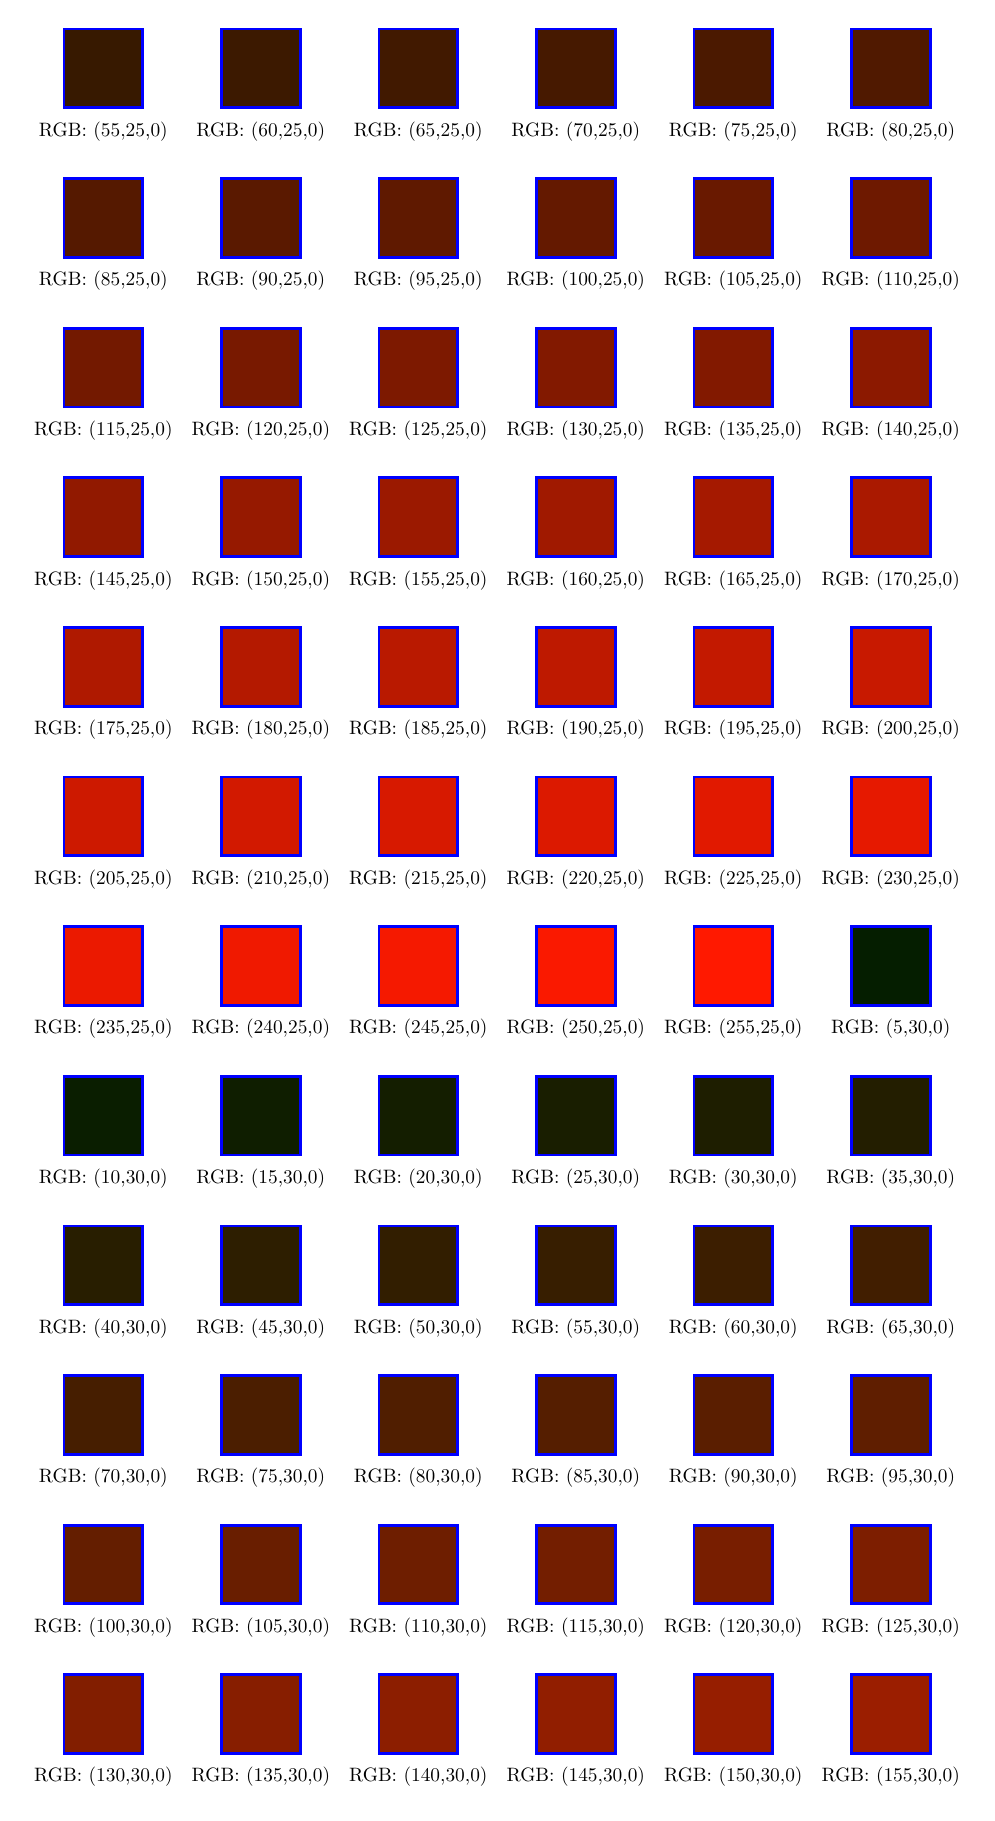
\begin{tikzpicture}

    \filldraw[draw=blue,line width=1,fill=colorR55G25B0]
    (0,0) rectangle (1,1);

    \node[scale=0.7] at (0.5,-0.3) {RGB: (55,25,0)};



    \begin{scope}[xshift=2cm]

      \filldraw[draw=blue,line width=1,fill=colorR60G25B0]
      (0,0) rectangle (1,1);

      \node[scale=0.7] at (0.5,-0.3) {RGB: (60,25,0)};

    \end{scope}



    \begin{scope}[xshift=4cm]

      \filldraw[draw=blue,line width=1,fill=colorR65G25B0]
      (0,0) rectangle (1,1);

      \node[scale=0.7] at (0.5,-0.3) {RGB: (65,25,0)};

    \end{scope}



    \begin{scope}[xshift=6cm]

      \filldraw[draw=blue,line width=1,fill=colorR70G25B0]
      (0,0) rectangle (1,1);

      \node[scale=0.7] at (0.5,-0.3) {RGB: (70,25,0)};

    \end{scope}



    \begin{scope}[xshift=8cm]

      \filldraw[draw=blue,line width=1,fill=colorR75G25B0]
      (0,0) rectangle (1,1);

      \node[scale=0.7] at (0.5,-0.3) {RGB: (75,25,0)};

    \end{scope}



    \begin{scope}[xshift=10cm]

      \filldraw[draw=blue,line width=1,fill=colorR80G25B0]
      (0,0) rectangle (1,1);

      \node[scale=0.7] at (0.5,-0.3) {RGB: (80,25,0)};

    \end{scope}







    \begin{scope}[yshift=-1.9cm]

      \filldraw[draw=blue,line width=1,fill=colorR85G25B0]
      (0,0) rectangle (1,1);

      \node[scale=0.7] at (0.5,-0.3) {RGB: (85,25,0)};

    \end{scope}



    \begin{scope}[xshift=2cm,yshift=-1.9cm]

      \filldraw[draw=blue,line width=1,fill=colorR90G25B0]
      (0,0) rectangle (1,1);

      \node[scale=0.7] at (0.5,-0.3) {RGB: (90,25,0)};

    \end{scope}



    \begin{scope}[xshift=4cm,yshift=-1.9cm]

      \filldraw[draw=blue,line width=1,fill=colorR95G25B0]
      (0,0) rectangle (1,1);

      \node[scale=0.7] at (0.5,-0.3) {RGB: (95,25,0)};

    \end{scope}



    \begin{scope}[xshift=6cm,yshift=-1.9cm]

      \filldraw[draw=blue,line width=1,fill=colorR100G25B0]
      (0,0) rectangle (1,1);

      \node[scale=0.7] at (0.5,-0.3) {RGB: (100,25,0)};

    \end{scope}



    \begin{scope}[xshift=8cm,yshift=-1.9cm]

      \filldraw[draw=blue,line width=1,fill=colorR105G25B0]
      (0,0) rectangle (1,1);

      \node[scale=0.7] at (0.5,-0.3) {RGB: (105,25,0)};

    \end{scope}



    \begin{scope}[xshift=10cm,yshift=-1.9cm]

      \filldraw[draw=blue,line width=1,fill=colorR110G25B0]
      (0,0) rectangle (1,1);

      \node[scale=0.7] at (0.5,-0.3) {RGB: (110,25,0)};

    \end{scope}







    \begin{scope}[yshift=-3.8cm]

      \filldraw[draw=blue,line width=1,fill=colorR115G25B0]
      (0,0) rectangle (1,1);

      \node[scale=0.7] at (0.5,-0.3) {RGB: (115,25,0)};

    \end{scope}



    \begin{scope}[xshift=2cm,yshift=-3.8cm]

      \filldraw[draw=blue,line width=1,fill=colorR120G25B0]
      (0,0) rectangle (1,1);

      \node[scale=0.7] at (0.5,-0.3) {RGB: (120,25,0)};

    \end{scope}



    \begin{scope}[xshift=4cm,yshift=-3.8cm]

      \filldraw[draw=blue,line width=1,fill=colorR125G25B0]
      (0,0) rectangle (1,1);

      \node[scale=0.7] at (0.5,-0.3) {RGB: (125,25,0)};

    \end{scope}



    \begin{scope}[xshift=6cm,yshift=-3.8cm]

      \filldraw[draw=blue,line width=1,fill=colorR130G25B0]
      (0,0) rectangle (1,1);

      \node[scale=0.7] at (0.5,-0.3) {RGB: (130,25,0)};

    \end{scope}



    \begin{scope}[xshift=8cm,yshift=-3.8cm]

      \filldraw[draw=blue,line width=1,fill=colorR130G25B0]
      (0,0) rectangle (1,1);

      \node[scale=0.7] at (0.5,-0.3) {RGB: (135,25,0)};

    \end{scope}



    \begin{scope}[xshift=10cm,yshift=-3.8cm]

      \filldraw[draw=blue,line width=1,fill=colorR140G25B0]
      (0,0) rectangle (1,1);

      \node[scale=0.7] at (0.5,-0.3) {RGB: (140,25,0)};

    \end{scope}







    \begin{scope}[yshift=-5.7cm]

      \filldraw[draw=blue,line width=1,fill=colorR145G25B0]
      (0,0) rectangle (1,1);

      \node[scale=0.7] at (0.5,-0.3) {RGB: (145,25,0)};

    \end{scope}



    \begin{scope}[xshift=2cm,yshift=-5.7cm]

      \filldraw[draw=blue,line width=1,fill=colorR150G25B0]
      (0,0) rectangle (1,1);

      \node[scale=0.7] at (0.5,-0.3) {RGB: (150,25,0)};

    \end{scope}



    \begin{scope}[xshift=4cm,yshift=-5.7cm]

      \filldraw[draw=blue,line width=1,fill=colorR155G25B0]
      (0,0) rectangle (1,1);

      \node[scale=0.7] at (0.5,-0.3) {RGB: (155,25,0)};

    \end{scope}



    \begin{scope}[xshift=6cm,yshift=-5.7cm]

      \filldraw[draw=blue,line width=1,fill=colorR160G25B0]
      (0,0) rectangle (1,1);

      \node[scale=0.7] at (0.5,-0.3) {RGB: (160,25,0)};

    \end{scope}



    \begin{scope}[xshift=8cm,yshift=-5.7cm]

      \filldraw[draw=blue,line width=1,fill=colorR165G25B0]
      (0,0) rectangle (1,1);

      \node[scale=0.7] at (0.5,-0.3) {RGB: (165,25,0)};

    \end{scope}



    \begin{scope}[xshift=10cm,yshift=-5.7cm]

      \filldraw[draw=blue,line width=1,fill=colorR170G25B0]
      (0,0) rectangle (1,1);

      \node[scale=0.7] at (0.5,-0.3) {RGB: (170,25,0)};

    \end{scope}







    \begin{scope}[yshift=-7.6cm]

      \filldraw[draw=blue,line width=1,fill=colorR175G25B0]
      (0,0) rectangle (1,1);

      \node[scale=0.7] at (0.5,-0.3) {RGB: (175,25,0)};

    \end{scope}



    \begin{scope}[xshift=2cm,yshift=-7.6cm]

      \filldraw[draw=blue,line width=1,fill=colorR180G25B0]
      (0,0) rectangle (1,1);

      \node[scale=0.7] at (0.5,-0.3) {RGB: (180,25,0)};

    \end{scope}



    \begin{scope}[xshift=4cm,yshift=-7.6cm]

      \filldraw[draw=blue,line width=1,fill=colorR185G25B0]
      (0,0) rectangle (1,1);

      \node[scale=0.7] at (0.5,-0.3) {RGB: (185,25,0)};

    \end{scope}



    \begin{scope}[xshift=6cm,yshift=-7.6cm]

      \filldraw[draw=blue,line width=1,fill=colorR190G25B0]
      (0,0) rectangle (1,1);

      \node[scale=0.7] at (0.5,-0.3) {RGB: (190,25,0)};

    \end{scope}



    \begin{scope}[xshift=8cm,yshift=-7.6cm]

      \filldraw[draw=blue,line width=1,fill=colorR195G25B0]
      (0,0) rectangle (1,1);

      \node[scale=0.7] at (0.5,-0.3) {RGB: (195,25,0)};

    \end{scope}



    \begin{scope}[xshift=10cm,yshift=-7.6cm]

      \filldraw[draw=blue,line width=1,fill=colorR200G25B0]
      (0,0) rectangle (1,1);

      \node[scale=0.7] at (0.5,-0.3) {RGB: (200,25,0)};

    \end{scope}







    \begin{scope}[yshift=-9.5cm]

      \filldraw[draw=blue,line width=1,fill=colorR205G25B0]
      (0,0) rectangle (1,1);

      \node[scale=0.7] at (0.5,-0.3) {RGB: (205,25,0)};

    \end{scope}



    \begin{scope}[xshift=2cm,yshift=-9.5cm]

      \filldraw[draw=blue,line width=1,fill=colorR210G25B0]
      (0,0) rectangle (1,1);

      \node[scale=0.7] at (0.5,-0.3) {RGB: (210,25,0)};

    \end{scope}



    \begin{scope}[xshift=4cm,yshift=-9.5cm]

      \filldraw[draw=blue,line width=1,fill=colorR215G25B0]
      (0,0) rectangle (1,1);

      \node[scale=0.7] at (0.5,-0.3) {RGB: (215,25,0)};

    \end{scope}



    \begin{scope}[xshift=6cm,yshift=-9.5cm]

      \filldraw[draw=blue,line width=1,fill=colorR220G25B0]
      (0,0) rectangle (1,1);

      \node[scale=0.7] at (0.5,-0.3) {RGB: (220,25,0)};

    \end{scope}



    \begin{scope}[xshift=8cm,yshift=-9.5cm]

      \filldraw[draw=blue,line width=1,fill=colorR225G25B0]
      (0,0) rectangle (1,1);

      \node[scale=0.7] at (0.5,-0.3) {RGB: (225,25,0)};

    \end{scope}



    \begin{scope}[xshift=10cm,yshift=-9.5cm]

      \filldraw[draw=blue,line width=1,fill=colorR230G25B0]
      (0,0) rectangle (1,1);

      \node[scale=0.7] at (0.5,-0.3) {RGB: (230,25,0)};

    \end{scope}







    \begin{scope}[yshift=-11.4cm]

      \filldraw[draw=blue,line width=1,fill=colorR235G25B0]
      (0,0) rectangle (1,1);

      \node[scale=0.7] at (0.5,-0.3) {RGB: (235,25,0)};

    \end{scope}



    \begin{scope}[xshift=2cm,yshift=-11.4cm]

      \filldraw[draw=blue,line width=1,fill=colorR240G25B0]
      (0,0) rectangle (1,1);

      \node[scale=0.7] at (0.5,-0.3) {RGB: (240,25,0)};

    \end{scope}



    \begin{scope}[xshift=4cm,yshift=-11.4cm]

      \filldraw[draw=blue,line width=1,fill=colorR245G25B0]
      (0,0) rectangle (1,1);

      \node[scale=0.7] at (0.5,-0.3) {RGB: (245,25,0)};

    \end{scope}



    \begin{scope}[xshift=6cm,yshift=-11.4cm]

      \filldraw[draw=blue,line width=1,fill=colorR250G25B0]
      (0,0) rectangle (1,1);

      \node[scale=0.7] at (0.5,-0.3) {RGB: (250,25,0)};

    \end{scope}



    \begin{scope}[xshift=8cm,yshift=-11.4cm]

      \filldraw[draw=blue,line width=1,fill=colorR255G25B0]
      (0,0) rectangle (1,1);

      \node[scale=0.7] at (0.5,-0.3) {RGB: (255,25,0)};

    \end{scope}



    \begin{scope}[xshift=10cm,yshift=-11.4cm]

      \filldraw[draw=blue,line width=1,fill=colorR5G30B0]
      (0,0) rectangle (1,1);

      \node[scale=0.7] at (0.5,-0.3) {RGB: (5,30,0)};

    \end{scope}







    \begin{scope}[yshift=-13.3cm]

      \filldraw[draw=blue,line width=1,fill=colorR10G30B0]
      (0,0) rectangle (1,1);

      \node[scale=0.7] at (0.5,-0.3) {RGB: (10,30,0)};

    \end{scope}



    \begin{scope}[xshift=2cm,yshift=-13.3cm]

      \filldraw[draw=blue,line width=1,fill=colorR15G30B0]
      (0,0) rectangle (1,1);

      \node[scale=0.7] at (0.5,-0.3) {RGB: (15,30,0)};

    \end{scope}



    \begin{scope}[xshift=4cm,yshift=-13.3cm]

      \filldraw[draw=blue,line width=1,fill=colorR20G30B0]
      (0,0) rectangle (1,1);

      \node[scale=0.7] at (0.5,-0.3) {RGB: (20,30,0)};

    \end{scope}



    \begin{scope}[xshift=6cm,yshift=-13.3cm]

      \filldraw[draw=blue,line width=1,fill=colorR25G30B0]
      (0,0) rectangle (1,1);

      \node[scale=0.7] at (0.5,-0.3) {RGB: (25,30,0)};

    \end{scope}



    \begin{scope}[xshift=8cm,yshift=-13.3cm]

      \filldraw[draw=blue,line width=1,fill=colorR30G30B0]
      (0,0) rectangle (1,1);

      \node[scale=0.7] at (0.5,-0.3) {RGB: (30,30,0)};

    \end{scope}



    \begin{scope}[xshift=10cm,yshift=-13.3cm]

      \filldraw[draw=blue,line width=1,fill=colorR35G30B0]
      (0,0) rectangle (1,1);

      \node[scale=0.7] at (0.5,-0.3) {RGB: (35,30,0)};

    \end{scope}







    \begin{scope}[yshift=-15.2cm]

      \filldraw[draw=blue,line width=1,fill=colorR40G30B0]
      (0,0) rectangle (1,1);

      \node[scale=0.7] at (0.5,-0.3) {RGB: (40,30,0)};

    \end{scope}



    \begin{scope}[xshift=2cm,yshift=-15.2cm]

      \filldraw[draw=blue,line width=1,fill=colorR45G30B0]
      (0,0) rectangle (1,1);

      \node[scale=0.7] at (0.5,-0.3) {RGB: (45,30,0)};

    \end{scope}



    \begin{scope}[xshift=4cm,yshift=-15.2cm]

      \filldraw[draw=blue,line width=1,fill=colorR50G30B0]
      (0,0) rectangle (1,1);

      \node[scale=0.7] at (0.5,-0.3) {RGB: (50,30,0)};

    \end{scope}



    \begin{scope}[xshift=6cm,yshift=-15.2cm]

      \filldraw[draw=blue,line width=1,fill=colorR55G30B0]
      (0,0) rectangle (1,1);

      \node[scale=0.7] at (0.5,-0.3) {RGB: (55,30,0)};

    \end{scope}



    \begin{scope}[xshift=8cm,yshift=-15.2cm]

      \filldraw[draw=blue,line width=1,fill=colorR60G30B0]
      (0,0) rectangle (1,1);

      \node[scale=0.7] at (0.5,-0.3) {RGB: (60,30,0)};

    \end{scope}



    \begin{scope}[xshift=10cm,yshift=-15.2cm]

      \filldraw[draw=blue,line width=1,fill=colorR65G30B0]
      (0,0) rectangle (1,1);

      \node[scale=0.7] at (0.5,-0.3) {RGB: (65,30,0)};

    \end{scope}







    \begin{scope}[yshift=-17.1cm]

      \filldraw[draw=blue,line width=1,fill=colorR70G30B0]
      (0,0) rectangle (1,1);

      \node[scale=0.7] at (0.5,-0.3) {RGB: (70,30,0)};

    \end{scope}



    \begin{scope}[xshift=2cm,yshift=-17.1cm]

      \filldraw[draw=blue,line width=1,fill=colorR75G30B0]
      (0,0) rectangle (1,1);

      \node[scale=0.7] at (0.5,-0.3) {RGB: (75,30,0)};

    \end{scope}



    \begin{scope}[xshift=4cm,yshift=-17.1cm]

      \filldraw[draw=blue,line width=1,fill=colorR80G30B0]
      (0,0) rectangle (1,1);

      \node[scale=0.7] at (0.5,-0.3) {RGB: (80,30,0)};

    \end{scope}



    \begin{scope}[xshift=6cm,yshift=-17.1cm]

      \filldraw[draw=blue,line width=1,fill=colorR85G30B0]
      (0,0) rectangle (1,1);

      \node[scale=0.7] at (0.5,-0.3) {RGB: (85,30,0)};

    \end{scope}



    \begin{scope}[xshift=8cm,yshift=-17.1cm]

      \filldraw[draw=blue,line width=1,fill=colorR90G30B0]
      (0,0) rectangle (1,1);

      \node[scale=0.7] at (0.5,-0.3) {RGB: (90,30,0)};

    \end{scope}



    \begin{scope}[xshift=10cm,yshift=-17.1cm]

      \filldraw[draw=blue,line width=1,fill=colorR95G30B0]
      (0,0) rectangle (1,1);

      \node[scale=0.7] at (0.5,-0.3) {RGB: (95,30,0)};

    \end{scope}







    \begin{scope}[yshift=-19cm]

      \filldraw[draw=blue,line width=1,fill=colorR100G30B0]
      (0,0) rectangle (1,1);

      \node[scale=0.7] at (0.5,-0.3) {RGB: (100,30,0)};

    \end{scope}



    \begin{scope}[xshift=2cm,yshift=-19cm]

      \filldraw[draw=blue,line width=1,fill=colorR105G30B0]
      (0,0) rectangle (1,1);

      \node[scale=0.7] at (0.5,-0.3) {RGB: (105,30,0)};

    \end{scope}



    \begin{scope}[xshift=4cm,yshift=-19cm]

      \filldraw[draw=blue,line width=1,fill=colorR110G30B0]
      (0,0) rectangle (1,1);

      \node[scale=0.7] at (0.5,-0.3) {RGB: (110,30,0)};

    \end{scope}



    \begin{scope}[xshift=6cm,yshift=-19cm]

      \filldraw[draw=blue,line width=1,fill=colorR115G30B0]
      (0,0) rectangle (1,1);

      \node[scale=0.7] at (0.5,-0.3) {RGB: (115,30,0)};

    \end{scope}



    \begin{scope}[xshift=8cm,yshift=-19cm]

      \filldraw[draw=blue,line width=1,fill=colorR120G30B0]
      (0,0) rectangle (1,1);

      \node[scale=0.7] at (0.5,-0.3) {RGB: (120,30,0)};

    \end{scope}



    \begin{scope}[xshift=10cm,yshift=-19cm]

      \filldraw[draw=blue,line width=1,fill=colorR125G30B0]
      (0,0) rectangle (1,1);

      \node[scale=0.7] at (0.5,-0.3) {RGB: (125,30,0)};

    \end{scope}







    \begin{scope}[yshift=-20.9cm]

      \filldraw[draw=blue,line width=1,fill=colorR130G30B0]
      (0,0) rectangle (1,1);

      \node[scale=0.7] at (0.5,-0.3) {RGB: (130,30,0)};

    \end{scope}



    \begin{scope}[xshift=2cm,yshift=-20.9cm]

      \filldraw[draw=blue,line width=1,fill=colorR135G30B0]
      (0,0) rectangle (1,1);

      \node[scale=0.7] at (0.5,-0.3) {RGB: (135,30,0)};

    \end{scope}



    \begin{scope}[xshift=4cm,yshift=-20.9cm]

      \filldraw[draw=blue,line width=1,fill=colorR140G30B0]
      (0,0) rectangle (1,1);

      \node[scale=0.7] at (0.5,-0.3) {RGB: (140,30,0)};

    \end{scope}



    \begin{scope}[xshift=6cm,yshift=-20.9cm]

      \filldraw[draw=blue,line width=1,fill=colorR145G30B0]
      (0,0) rectangle (1,1);

      \node[scale=0.7] at (0.5,-0.3) {RGB: (145,30,0)};

    \end{scope}



    \begin{scope}[xshift=8cm,yshift=-20.9cm]

      \filldraw[draw=blue,line width=1,fill=colorR150G30B0]
      (0,0) rectangle (1,1);

      \node[scale=0.7] at (0.5,-0.3) {RGB: (150,30,0)};

    \end{scope}



    \begin{scope}[xshift=10cm,yshift=-20.9cm]

      \filldraw[draw=blue,line width=1,fill=colorR155G30B0]
      (0,0) rectangle (1,1);

      \node[scale=0.7] at (0.5,-0.3) {RGB: (155,30,0)};

    \end{scope}

  \end{tikzpicture}

  \caption{Mixed colors in~RGB system: $(55,25,0)$--$(255,25,0)$,
    $(5,30,0)$--$(155,30,0)$}



  \label{fig:Mixed-colors-Part-04}

\end{figure}
% ##################





% ##################
\begin{figure}

  \centering


  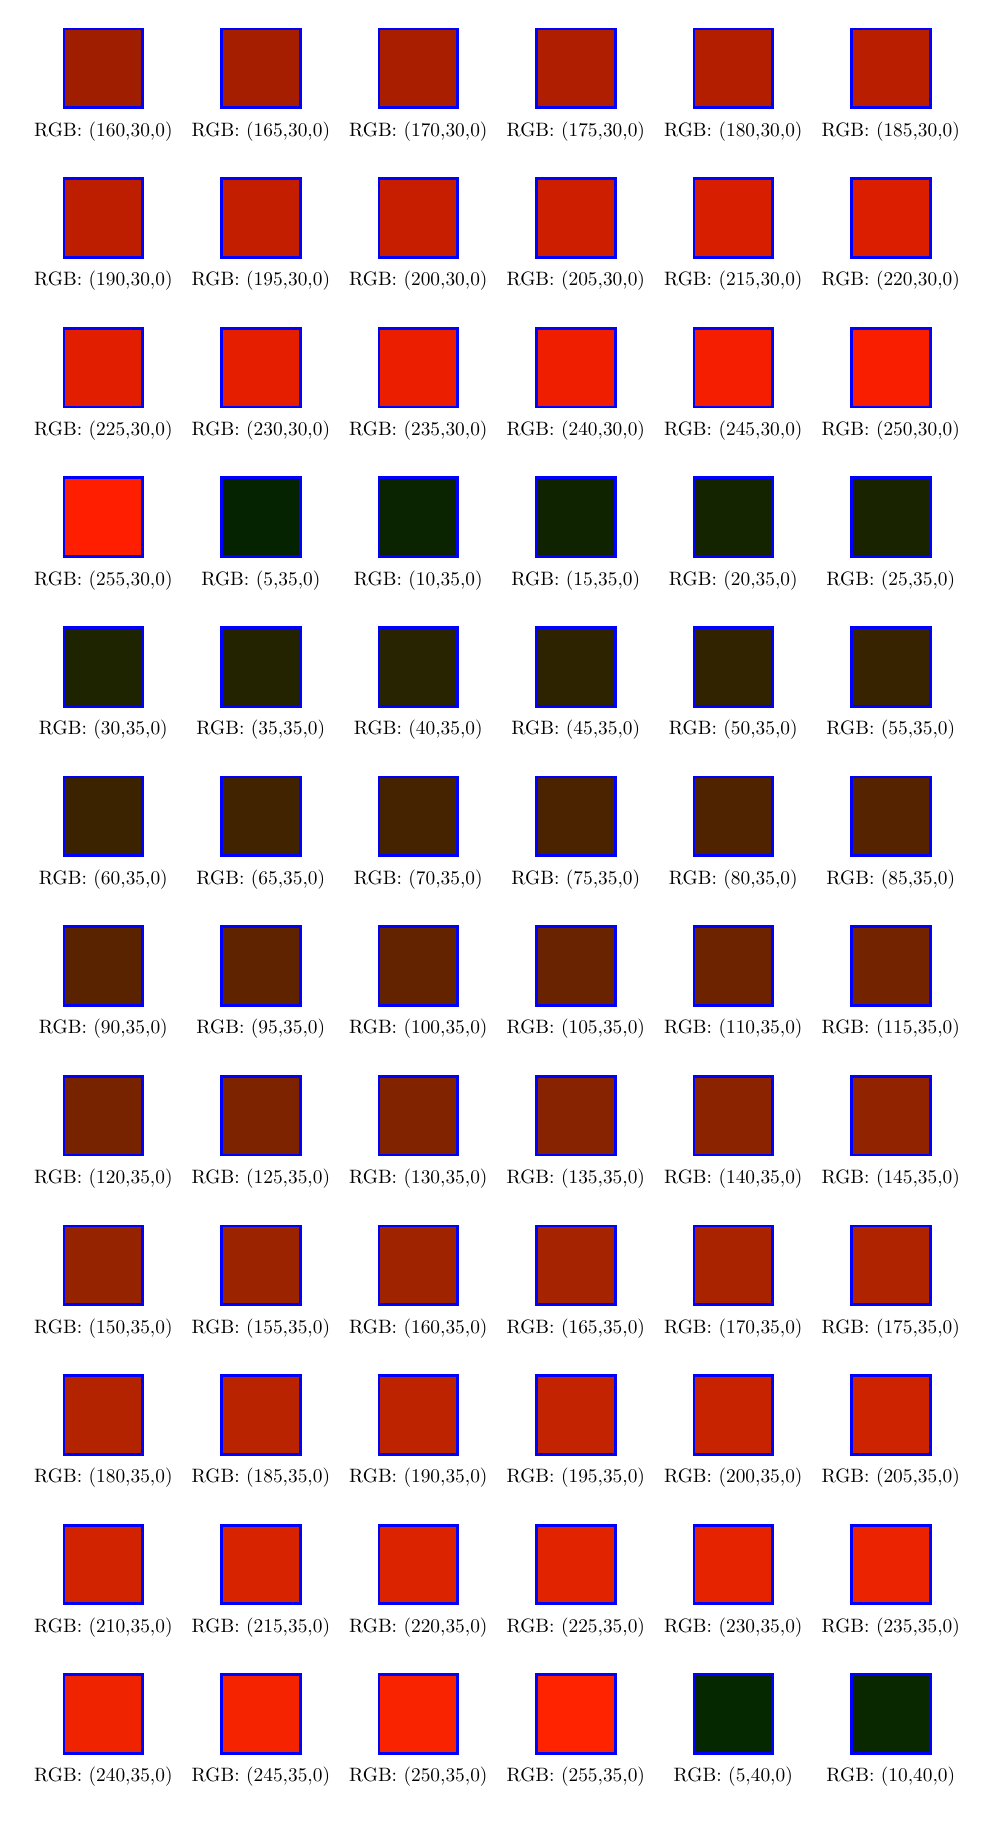
\begin{tikzpicture}

    \filldraw[draw=blue,line width=1,fill=colorR160G30B0]
    (0,0) rectangle (1,1);

    \node[scale=0.7] at (0.5,-0.3) {RGB: (160,30,0)};



    \begin{scope}[xshift=2cm]

      \filldraw[draw=blue,line width=1,fill=colorR165G30B0]
      (0,0) rectangle (1,1);

      \node[scale=0.7] at (0.5,-0.3) {RGB: (165,30,0)};

    \end{scope}



    \begin{scope}[xshift=4cm]

      \filldraw[draw=blue,line width=1,fill=colorR170G30B0]
      (0,0) rectangle (1,1);

      \node[scale=0.7] at (0.5,-0.3) {RGB: (170,30,0)};

    \end{scope}



    \begin{scope}[xshift=6cm]

      \filldraw[draw=blue,line width=1,fill=colorR175G30B0]
      (0,0) rectangle (1,1);

      \node[scale=0.7] at (0.5,-0.3) {RGB: (175,30,0)};

    \end{scope}



    \begin{scope}[xshift=8cm]

      \filldraw[draw=blue,line width=1,fill=colorR180G30B0]
      (0,0) rectangle (1,1);

      \node[scale=0.7] at (0.5,-0.3) {RGB: (180,30,0)};

    \end{scope}



    \begin{scope}[xshift=10cm]

      \filldraw[draw=blue,line width=1,fill=colorR185G30B0]
      (0,0) rectangle (1,1);

      \node[scale=0.7] at (0.5,-0.3) {RGB: (185,30,0)};

    \end{scope}







    \begin{scope}[yshift=-1.9cm]

      \filldraw[draw=blue,line width=1,fill=colorR190G30B0]
      (0,0) rectangle (1,1);

      \node[scale=0.7] at (0.5,-0.3) {RGB: (190,30,0)};

    \end{scope}



    \begin{scope}[xshift=2cm,yshift=-1.9cm]

      \filldraw[draw=blue,line width=1,fill=colorR195G30B0]
      (0,0) rectangle (1,1);

      \node[scale=0.7] at (0.5,-0.3) {RGB: (195,30,0)};

    \end{scope}



    \begin{scope}[xshift=4cm,yshift=-1.9cm]

      \filldraw[draw=blue,line width=1,fill=colorR200G30B0]
      (0,0) rectangle (1,1);

      \node[scale=0.7] at (0.5,-0.3) {RGB: (200,30,0)};

    \end{scope}



    \begin{scope}[xshift=6cm,yshift=-1.9cm]

      \filldraw[draw=blue,line width=1,fill=colorR205G30B0]
      (0,0) rectangle (1,1);

      \node[scale=0.7] at (0.5,-0.3) {RGB: (205,30,0)};

    \end{scope}



    \begin{scope}[xshift=8cm,yshift=-1.9cm]

      \filldraw[draw=blue,line width=1,fill=colorR215G30B0]
      (0,0) rectangle (1,1);

      \node[scale=0.7] at (0.5,-0.3) {RGB: (215,30,0)};

    \end{scope}



    \begin{scope}[xshift=10cm,yshift=-1.9cm]

      \filldraw[draw=blue,line width=1,fill=colorR220G30B0]
      (0,0) rectangle (1,1);

      \node[scale=0.7] at (0.5,-0.3) {RGB: (220,30,0)};

    \end{scope}







    \begin{scope}[yshift=-3.8cm]

      \filldraw[draw=blue,line width=1,fill=colorR225G30B0]
      (0,0) rectangle (1,1);

      \node[scale=0.7] at (0.5,-0.3) {RGB: (225,30,0)};

    \end{scope}



    \begin{scope}[xshift=2cm,yshift=-3.8cm]

      \filldraw[draw=blue,line width=1,fill=colorR230G30B0]
      (0,0) rectangle (1,1);

      \node[scale=0.7] at (0.5,-0.3) {RGB: (230,30,0)};

    \end{scope}



    \begin{scope}[xshift=4cm,yshift=-3.8cm]

      \filldraw[draw=blue,line width=1,fill=colorR235G30B0]
      (0,0) rectangle (1,1);

      \node[scale=0.7] at (0.5,-0.3) {RGB: (235,30,0)};

    \end{scope}



    \begin{scope}[xshift=6cm,yshift=-3.8cm]

      \filldraw[draw=blue,line width=1,fill=colorR240G30B0]
      (0,0) rectangle (1,1);

      \node[scale=0.7] at (0.5,-0.3) {RGB: (240,30,0)};

    \end{scope}



    \begin{scope}[xshift=8cm,yshift=-3.8cm]

      \filldraw[draw=blue,line width=1,fill=colorR245G30B0]
      (0,0) rectangle (1,1);

      \node[scale=0.7] at (0.5,-0.3) {RGB: (245,30,0)};

    \end{scope}



    \begin{scope}[xshift=10cm,yshift=-3.8cm]

      \filldraw[draw=blue,line width=1,fill=colorR250G30B0]
      (0,0) rectangle (1,1);

      \node[scale=0.7] at (0.5,-0.3) {RGB: (250,30,0)};

    \end{scope}







    \begin{scope}[yshift=-5.7cm]

      \filldraw[draw=blue,line width=1,fill=colorR255G30B0]
      (0,0) rectangle (1,1);

      \node[scale=0.7] at (0.5,-0.3) {RGB: (255,30,0)};

    \end{scope}



    \begin{scope}[xshift=2cm,yshift=-5.7cm]

      \filldraw[draw=blue,line width=1,fill=colorR5G35B0]
      (0,0) rectangle (1,1);

      \node[scale=0.7] at (0.5,-0.3) {RGB: (5,35,0)};

    \end{scope}



    \begin{scope}[xshift=4cm,yshift=-5.7cm]

      \filldraw[draw=blue,line width=1,fill=colorR10G35B0]
      (0,0) rectangle (1,1);

      \node[scale=0.7] at (0.5,-0.3) {RGB: (10,35,0)};

    \end{scope}



    \begin{scope}[xshift=6cm,yshift=-5.7cm]

      \filldraw[draw=blue,line width=1,fill=colorR15G35B0]
      (0,0) rectangle (1,1);

      \node[scale=0.7] at (0.5,-0.3) {RGB: (15,35,0)};

    \end{scope}



    \begin{scope}[xshift=8cm,yshift=-5.7cm]

      \filldraw[draw=blue,line width=1,fill=colorR20G35B0]
      (0,0) rectangle (1,1);

      \node[scale=0.7] at (0.5,-0.3) {RGB: (20,35,0)};

    \end{scope}



    \begin{scope}[xshift=10cm,yshift=-5.7cm]

      \filldraw[draw=blue,line width=1,fill=colorR25G35B0]
      (0,0) rectangle (1,1);

      \node[scale=0.7] at (0.5,-0.3) {RGB: (25,35,0)};

    \end{scope}







    \begin{scope}[yshift=-7.6cm]

      \filldraw[draw=blue,line width=1,fill=colorR30G35B0]
      (0,0) rectangle (1,1);

      \node[scale=0.7] at (0.5,-0.3) {RGB: (30,35,0)};

    \end{scope}



    \begin{scope}[xshift=2cm,yshift=-7.6cm]

      \filldraw[draw=blue,line width=1,fill=colorR35G35B0]
      (0,0) rectangle (1,1);

      \node[scale=0.7] at (0.5,-0.3) {RGB: (35,35,0)};

    \end{scope}



    \begin{scope}[xshift=4cm,yshift=-7.6cm]

      \filldraw[draw=blue,line width=1,fill=colorR40G35B0]
      (0,0) rectangle (1,1);

      \node[scale=0.7] at (0.5,-0.3) {RGB: (40,35,0)};

    \end{scope}



    \begin{scope}[xshift=6cm,yshift=-7.6cm]

      \filldraw[draw=blue,line width=1,fill=colorR45G35B0]
      (0,0) rectangle (1,1);

      \node[scale=0.7] at (0.5,-0.3) {RGB: (45,35,0)};

    \end{scope}



    \begin{scope}[xshift=8cm,yshift=-7.6cm]

      \filldraw[draw=blue,line width=1,fill=colorR50G35B0]
      (0,0) rectangle (1,1);

      \node[scale=0.7] at (0.5,-0.3) {RGB: (50,35,0)};

    \end{scope}



    \begin{scope}[xshift=10cm,yshift=-7.6cm]

      \filldraw[draw=blue,line width=1,fill=colorR55G35B0]
      (0,0) rectangle (1,1);

      \node[scale=0.7] at (0.5,-0.3) {RGB: (55,35,0)};

    \end{scope}







    \begin{scope}[yshift=-9.5cm]

      \filldraw[draw=blue,line width=1,fill=colorR60G35B0]
      (0,0) rectangle (1,1);

      \node[scale=0.7] at (0.5,-0.3) {RGB: (60,35,0)};

    \end{scope}



    \begin{scope}[xshift=2cm,yshift=-9.5cm]

      \filldraw[draw=blue,line width=1,fill=colorR65G35B0]
      (0,0) rectangle (1,1);

      \node[scale=0.7] at (0.5,-0.3) {RGB: (65,35,0)};

    \end{scope}



    \begin{scope}[xshift=4cm,yshift=-9.5cm]

      \filldraw[draw=blue,line width=1,fill=colorR70G35B0]
      (0,0) rectangle (1,1);

      \node[scale=0.7] at (0.5,-0.3) {RGB: (70,35,0)};

    \end{scope}



    \begin{scope}[xshift=6cm,yshift=-9.5cm]

      \filldraw[draw=blue,line width=1,fill=colorR75G35B0]
      (0,0) rectangle (1,1);

      \node[scale=0.7] at (0.5,-0.3) {RGB: (75,35,0)};

    \end{scope}



    \begin{scope}[xshift=8cm,yshift=-9.5cm]

      \filldraw[draw=blue,line width=1,fill=colorR80G35B0]
      (0,0) rectangle (1,1);

      \node[scale=0.7] at (0.5,-0.3) {RGB: (80,35,0)};

    \end{scope}



    \begin{scope}[xshift=10cm,yshift=-9.5cm]

      \filldraw[draw=blue,line width=1,fill=colorR85G35B0]
      (0,0) rectangle (1,1);

      \node[scale=0.7] at (0.5,-0.3) {RGB: (85,35,0)};

    \end{scope}







    \begin{scope}[yshift=-11.4cm]

      \filldraw[draw=blue,line width=1,fill=colorR90G35B0]
      (0,0) rectangle (1,1);

      \node[scale=0.7] at (0.5,-0.3) {RGB: (90,35,0)};

    \end{scope}



    \begin{scope}[xshift=2cm,yshift=-11.4cm]

      \filldraw[draw=blue,line width=1,fill=colorR95G35B0]
      (0,0) rectangle (1,1);

      \node[scale=0.7] at (0.5,-0.3) {RGB: (95,35,0)};

    \end{scope}



    \begin{scope}[xshift=4cm,yshift=-11.4cm]

      \filldraw[draw=blue,line width=1,fill=colorR100G35B0]
      (0,0) rectangle (1,1);

      \node[scale=0.7] at (0.5,-0.3) {RGB: (100,35,0)};

    \end{scope}



    \begin{scope}[xshift=6cm,yshift=-11.4cm]

      \filldraw[draw=blue,line width=1,fill=colorR105G35B0]
      (0,0) rectangle (1,1);

      \node[scale=0.7] at (0.5,-0.3) {RGB: (105,35,0)};

    \end{scope}



    \begin{scope}[xshift=8cm,yshift=-11.4cm]

      \filldraw[draw=blue,line width=1,fill=colorR110G35B0]
      (0,0) rectangle (1,1);

      \node[scale=0.7] at (0.5,-0.3) {RGB: (110,35,0)};

    \end{scope}



    \begin{scope}[xshift=10cm,yshift=-11.4cm]

      \filldraw[draw=blue,line width=1,fill=colorR115G35B0]
      (0,0) rectangle (1,1);

      \node[scale=0.7] at (0.5,-0.3) {RGB: (115,35,0)};

    \end{scope}







    \begin{scope}[yshift=-13.3cm]

      \filldraw[draw=blue,line width=1,fill=colorR120G35B0]
      (0,0) rectangle (1,1);

      \node[scale=0.7] at (0.5,-0.3) {RGB: (120,35,0)};

    \end{scope}



    \begin{scope}[xshift=2cm,yshift=-13.3cm]

      \filldraw[draw=blue,line width=1,fill=colorR125G35B0]
      (0,0) rectangle (1,1);

      \node[scale=0.7] at (0.5,-0.3) {RGB: (125,35,0)};

    \end{scope}



    \begin{scope}[xshift=4cm,yshift=-13.3cm]

      \filldraw[draw=blue,line width=1,fill=colorR130G35B0]
      (0,0) rectangle (1,1);

      \node[scale=0.7] at (0.5,-0.3) {RGB: (130,35,0)};

    \end{scope}



    \begin{scope}[xshift=6cm,yshift=-13.3cm]

      \filldraw[draw=blue,line width=1,fill=colorR135G35B0]
      (0,0) rectangle (1,1);

      \node[scale=0.7] at (0.5,-0.3) {RGB: (135,35,0)};

    \end{scope}



    \begin{scope}[xshift=8cm,yshift=-13.3cm]

      \filldraw[draw=blue,line width=1,fill=colorR140G35B0]
      (0,0) rectangle (1,1);

      \node[scale=0.7] at (0.5,-0.3) {RGB: (140,35,0)};

    \end{scope}



    \begin{scope}[xshift=10cm,yshift=-13.3cm]

      \filldraw[draw=blue,line width=1,fill=colorR145G35B0]
      (0,0) rectangle (1,1);

      \node[scale=0.7] at (0.5,-0.3) {RGB: (145,35,0)};

    \end{scope}







    \begin{scope}[yshift=-15.2cm]

      \filldraw[draw=blue,line width=1,fill=colorR150G35B0]
      (0,0) rectangle (1,1);

      \node[scale=0.7] at (0.5,-0.3) {RGB: (150,35,0)};

    \end{scope}



    \begin{scope}[xshift=2cm,yshift=-15.2cm]

      \filldraw[draw=blue,line width=1,fill=colorR155G35B0]
      (0,0) rectangle (1,1);

      \node[scale=0.7] at (0.5,-0.3) {RGB: (155,35,0)};

    \end{scope}



    \begin{scope}[xshift=4cm,yshift=-15.2cm]

      \filldraw[draw=blue,line width=1,fill=colorR160G35B0]
      (0,0) rectangle (1,1);

      \node[scale=0.7] at (0.5,-0.3) {RGB: (160,35,0)};

    \end{scope}



    \begin{scope}[xshift=6cm,yshift=-15.2cm]

      \filldraw[draw=blue,line width=1,fill=colorR165G35B0]
      (0,0) rectangle (1,1);

      \node[scale=0.7] at (0.5,-0.3) {RGB: (165,35,0)};

    \end{scope}



    \begin{scope}[xshift=8cm,yshift=-15.2cm]

      \filldraw[draw=blue,line width=1,fill=colorR170G35B0]
      (0,0) rectangle (1,1);

      \node[scale=0.7] at (0.5,-0.3) {RGB: (170,35,0)};

    \end{scope}



    \begin{scope}[xshift=10cm,yshift=-15.2cm]

      \filldraw[draw=blue,line width=1,fill=colorR175G35B0]
      (0,0) rectangle (1,1);

      \node[scale=0.7] at (0.5,-0.3) {RGB: (175,35,0)};

    \end{scope}







    \begin{scope}[yshift=-17.1cm]

      \filldraw[draw=blue,line width=1,fill=colorR180G35B0]
      (0,0) rectangle (1,1);

      \node[scale=0.7] at (0.5,-0.3) {RGB: (180,35,0)};

    \end{scope}



    \begin{scope}[xshift=2cm,yshift=-17.1cm]

      \filldraw[draw=blue,line width=1,fill=colorR185G35B0]
      (0,0) rectangle (1,1);

      \node[scale=0.7] at (0.5,-0.3) {RGB: (185,35,0)};

    \end{scope}



    \begin{scope}[xshift=4cm,yshift=-17.1cm]

      \filldraw[draw=blue,line width=1,fill=colorR190G35B0]
      (0,0) rectangle (1,1);

      \node[scale=0.7] at (0.5,-0.3) {RGB: (190,35,0)};

    \end{scope}



    \begin{scope}[xshift=6cm,yshift=-17.1cm]

      \filldraw[draw=blue,line width=1,fill=colorR195G35B0]
      (0,0) rectangle (1,1);

      \node[scale=0.7] at (0.5,-0.3) {RGB: (195,35,0)};

    \end{scope}



    \begin{scope}[xshift=8cm,yshift=-17.1cm]

      \filldraw[draw=blue,line width=1,fill=colorR200G35B0]
      (0,0) rectangle (1,1);

      \node[scale=0.7] at (0.5,-0.3) {RGB: (200,35,0)};

    \end{scope}



    \begin{scope}[xshift=10cm,yshift=-17.1cm]

      \filldraw[draw=blue,line width=1,fill=colorR205G35B0]
      (0,0) rectangle (1,1);

      \node[scale=0.7] at (0.5,-0.3) {RGB: (205,35,0)};

    \end{scope}







    \begin{scope}[yshift=-19cm]

      \filldraw[draw=blue,line width=1,fill=colorR210G35B0]
      (0,0) rectangle (1,1);

      \node[scale=0.7] at (0.5,-0.3) {RGB: (210,35,0)};

    \end{scope}



    \begin{scope}[xshift=2cm,yshift=-19cm]

      \filldraw[draw=blue,line width=1,fill=colorR215G35B0]
      (0,0) rectangle (1,1);

      \node[scale=0.7] at (0.5,-0.3) {RGB: (215,35,0)};

    \end{scope}



    \begin{scope}[xshift=4cm,yshift=-19cm]

      \filldraw[draw=blue,line width=1,fill=colorR220G35B0]
      (0,0) rectangle (1,1);

      \node[scale=0.7] at (0.5,-0.3) {RGB: (220,35,0)};

    \end{scope}



    \begin{scope}[xshift=6cm,yshift=-19cm]

      \filldraw[draw=blue,line width=1,fill=colorR225G35B0]
      (0,0) rectangle (1,1);

      \node[scale=0.7] at (0.5,-0.3) {RGB: (225,35,0)};

    \end{scope}



    \begin{scope}[xshift=8cm,yshift=-19cm]

      \filldraw[draw=blue,line width=1,fill=colorR230G35B0]
      (0,0) rectangle (1,1);

      \node[scale=0.7] at (0.5,-0.3) {RGB: (230,35,0)};

    \end{scope}



    \begin{scope}[xshift=10cm,yshift=-19cm]

      \filldraw[draw=blue,line width=1,fill=colorR235G35B0]
      (0,0) rectangle (1,1);

      \node[scale=0.7] at (0.5,-0.3) {RGB: (235,35,0)};

    \end{scope}







    \begin{scope}[yshift=-20.9cm]

      \filldraw[draw=blue,line width=1,fill=colorR240G35B0]
      (0,0) rectangle (1,1);

      \node[scale=0.7] at (0.5,-0.3) {RGB: (240,35,0)};

    \end{scope}



    \begin{scope}[xshift=2cm,yshift=-20.9cm]

      \filldraw[draw=blue,line width=1,fill=colorR245G35B0]
      (0,0) rectangle (1,1);

      \node[scale=0.7] at (0.5,-0.3) {RGB: (245,35,0)};

    \end{scope}



    \begin{scope}[xshift=4cm,yshift=-20.9cm]

      \filldraw[draw=blue,line width=1,fill=colorR250G35B0]
      (0,0) rectangle (1,1);

      \node[scale=0.7] at (0.5,-0.3) {RGB: (250,35,0)};

    \end{scope}



    \begin{scope}[xshift=6cm,yshift=-20.9cm]

      \filldraw[draw=blue,line width=1,fill=colorR255G35B0]
      (0,0) rectangle (1,1);

      \node[scale=0.7] at (0.5,-0.3) {RGB: (255,35,0)};

    \end{scope}



    \begin{scope}[xshift=8cm,yshift=-20.9cm]

      \filldraw[draw=blue,line width=1,fill=colorR5G40B0]
      (0,0) rectangle (1,1);

      \node[scale=0.7] at (0.5,-0.3) {RGB: (5,40,0)};

    \end{scope}



    \begin{scope}[xshift=10cm,yshift=-20.9cm]

      \filldraw[draw=blue,line width=1,fill=colorR10G40B0]
      (0,0) rectangle (1,1);

      \node[scale=0.7] at (0.5,-0.3) {RGB: (10,40,0)};

    \end{scope}

  \end{tikzpicture}

  \caption{Mixed colors in~RGB system: $(160,30,0)$--$(255,30,0)$,
    $(5,35,0)$--$(255,35,0)$, $(5,40,0)$--$(10,40,0)$}



  \label{fig:Mixed-colors-Part-05}

\end{figure}
% ##################





% ##################
\begin{figure}

  \centering


  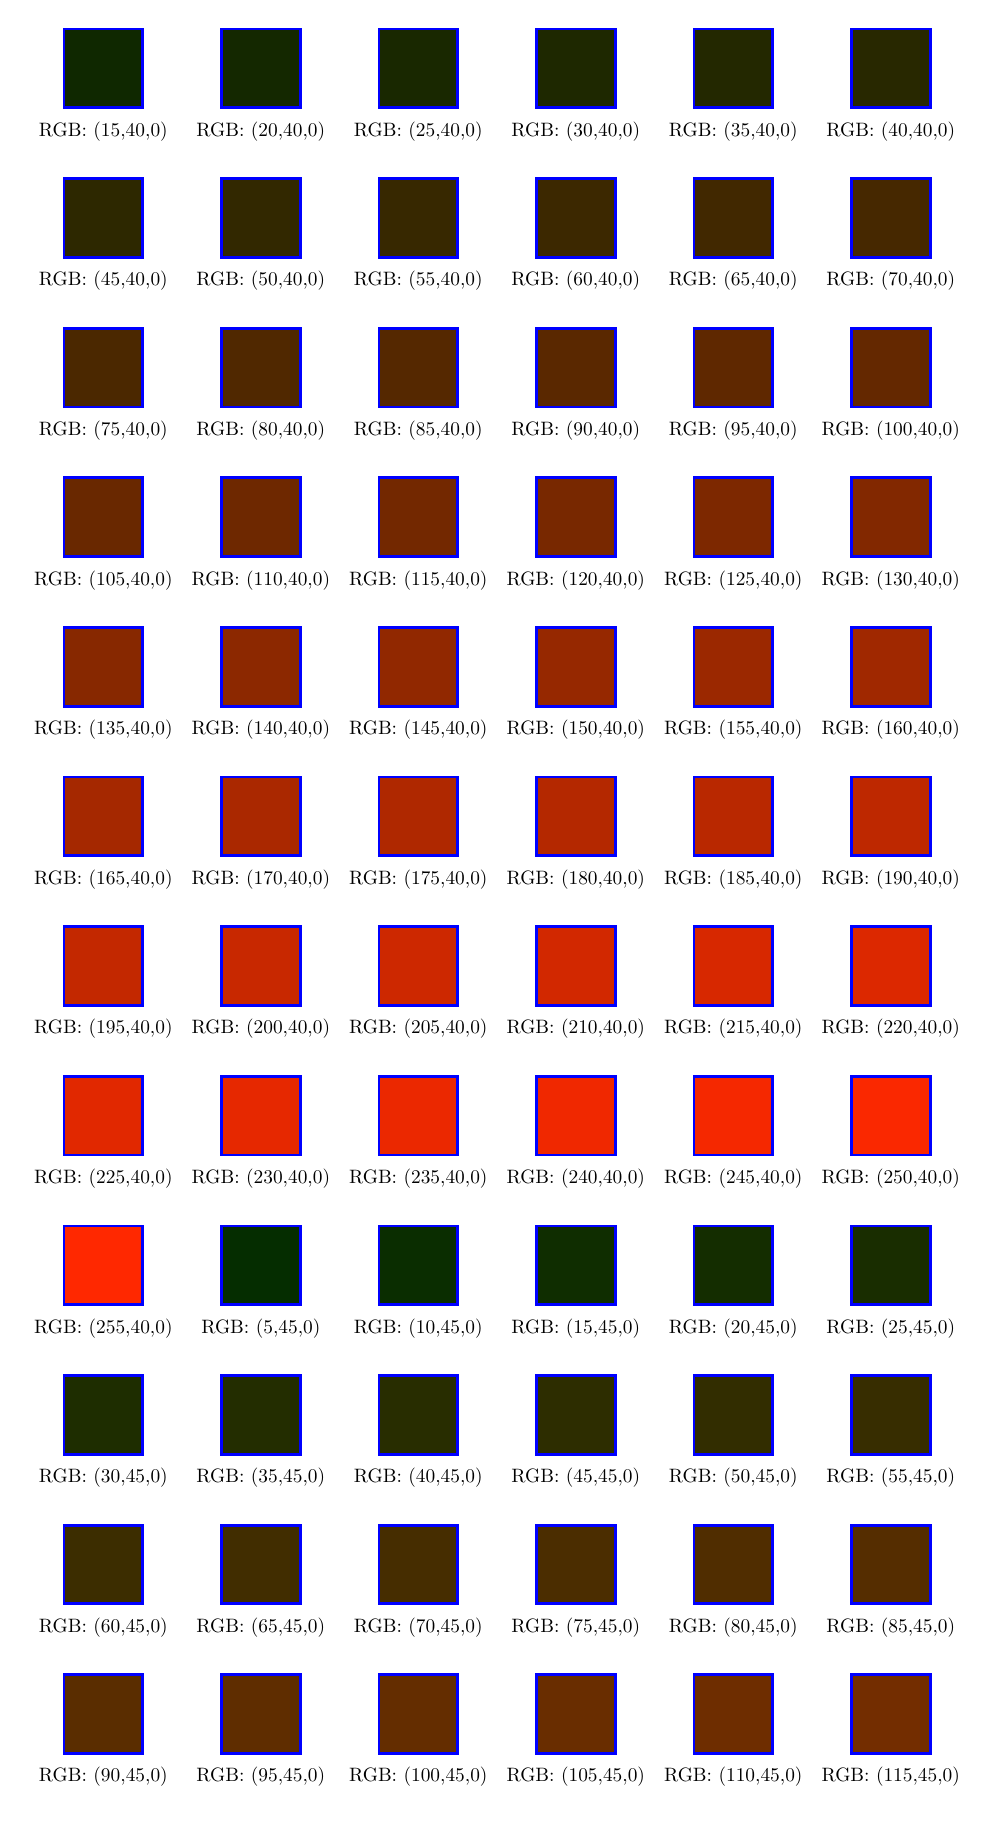
\begin{tikzpicture}

    \filldraw[draw=blue,line width=1,fill=colorR15G40B0]
    (0,0) rectangle (1,1);

    \node[scale=0.7] at (0.5,-0.3) {RGB: (15,40,0)};



    \begin{scope}[xshift=2cm]

      \filldraw[draw=blue,line width=1,fill=colorR20G40B0]
      (0,0) rectangle (1,1);

      \node[scale=0.7] at (0.5,-0.3) {RGB: (20,40,0)};

    \end{scope}



    \begin{scope}[xshift=4cm]

      \filldraw[draw=blue,line width=1,fill=colorR25G40B0]
      (0,0) rectangle (1,1);

      \node[scale=0.7] at (0.5,-0.3) {RGB: (25,40,0)};

    \end{scope}



    \begin{scope}[xshift=6cm]

      \filldraw[draw=blue,line width=1,fill=colorR30G40B0]
      (0,0) rectangle (1,1);

      \node[scale=0.7] at (0.5,-0.3) {RGB: (30,40,0)};

    \end{scope}



    \begin{scope}[xshift=8cm]

      \filldraw[draw=blue,line width=1,fill=colorR35G40B0]
      (0,0) rectangle (1,1);

      \node[scale=0.7] at (0.5,-0.3) {RGB: (35,40,0)};

    \end{scope}



    \begin{scope}[xshift=10cm]

      \filldraw[draw=blue,line width=1,fill=colorR40G40B0]
      (0,0) rectangle (1,1);

      \node[scale=0.7] at (0.5,-0.3) {RGB: (40,40,0)};

    \end{scope}







    \begin{scope}[yshift=-1.9cm]

      \filldraw[draw=blue,line width=1,fill=colorR45G40B0]
      (0,0) rectangle (1,1);

      \node[scale=0.7] at (0.5,-0.3) {RGB: (45,40,0)};

    \end{scope}



    \begin{scope}[xshift=2cm,yshift=-1.9cm]

      \filldraw[draw=blue,line width=1,fill=colorR50G40B0]
      (0,0) rectangle (1,1);

      \node[scale=0.7] at (0.5,-0.3) {RGB: (50,40,0)};

    \end{scope}



    \begin{scope}[xshift=4cm,yshift=-1.9cm]

      \filldraw[draw=blue,line width=1,fill=colorR55G40B0]
      (0,0) rectangle (1,1);

      \node[scale=0.7] at (0.5,-0.3) {RGB: (55,40,0)};

    \end{scope}



    \begin{scope}[xshift=6cm,yshift=-1.9cm]

      \filldraw[draw=blue,line width=1,fill=colorR60G40B0]
      (0,0) rectangle (1,1);

      \node[scale=0.7] at (0.5,-0.3) {RGB: (60,40,0)};

    \end{scope}



    \begin{scope}[xshift=8cm,yshift=-1.9cm]

      \filldraw[draw=blue,line width=1,fill=colorR65G40B0]
      (0,0) rectangle (1,1);

      \node[scale=0.7] at (0.5,-0.3) {RGB: (65,40,0)};

    \end{scope}



    \begin{scope}[xshift=10cm,yshift=-1.9cm]

      \filldraw[draw=blue,line width=1,fill=colorR70G40B0]
      (0,0) rectangle (1,1);

      \node[scale=0.7] at (0.5,-0.3) {RGB: (70,40,0)};

    \end{scope}







    \begin{scope}[yshift=-3.8cm]

      \filldraw[draw=blue,line width=1,fill=colorR75G40B0]
      (0,0) rectangle (1,1);

      \node[scale=0.7] at (0.5,-0.3) {RGB: (75,40,0)};

    \end{scope}



    \begin{scope}[xshift=2cm,yshift=-3.8cm]

      \filldraw[draw=blue,line width=1,fill=colorR80G40B0]
      (0,0) rectangle (1,1);

      \node[scale=0.7] at (0.5,-0.3) {RGB: (80,40,0)};

    \end{scope}



    \begin{scope}[xshift=4cm,yshift=-3.8cm]

      \filldraw[draw=blue,line width=1,fill=colorR85G40B0]
      (0,0) rectangle (1,1);

      \node[scale=0.7] at (0.5,-0.3) {RGB: (85,40,0)};

    \end{scope}



    \begin{scope}[xshift=6cm,yshift=-3.8cm]

      \filldraw[draw=blue,line width=1,fill=colorR90G40B0]
      (0,0) rectangle (1,1);

      \node[scale=0.7] at (0.5,-0.3) {RGB: (90,40,0)};

    \end{scope}



    \begin{scope}[xshift=8cm,yshift=-3.8cm]

      \filldraw[draw=blue,line width=1,fill=colorR95G40B0]
      (0,0) rectangle (1,1);

      \node[scale=0.7] at (0.5,-0.3) {RGB: (95,40,0)};

    \end{scope}



    \begin{scope}[xshift=10cm,yshift=-3.8cm]

      \filldraw[draw=blue,line width=1,fill=colorR100G40B0]
      (0,0) rectangle (1,1);

      \node[scale=0.7] at (0.5,-0.3) {RGB: (100,40,0)};

    \end{scope}







    \begin{scope}[yshift=-5.7cm]

      \filldraw[draw=blue,line width=1,fill=colorR105G40B0]
      (0,0) rectangle (1,1);

      \node[scale=0.7] at (0.5,-0.3) {RGB: (105,40,0)};

    \end{scope}



    \begin{scope}[xshift=2cm,yshift=-5.7cm]

      \filldraw[draw=blue,line width=1,fill=colorR110G40B0]
      (0,0) rectangle (1,1);

      \node[scale=0.7] at (0.5,-0.3) {RGB: (110,40,0)};

    \end{scope}



    \begin{scope}[xshift=4cm,yshift=-5.7cm]

      \filldraw[draw=blue,line width=1,fill=colorR115G40B0]
      (0,0) rectangle (1,1);

      \node[scale=0.7] at (0.5,-0.3) {RGB: (115,40,0)};

    \end{scope}



    \begin{scope}[xshift=6cm,yshift=-5.7cm]

      \filldraw[draw=blue,line width=1,fill=colorR120G40B0]
      (0,0) rectangle (1,1);

      \node[scale=0.7] at (0.5,-0.3) {RGB: (120,40,0)};

    \end{scope}



    \begin{scope}[xshift=8cm,yshift=-5.7cm]

      \filldraw[draw=blue,line width=1,fill=colorR125G40B0]
      (0,0) rectangle (1,1);

      \node[scale=0.7] at (0.5,-0.3) {RGB: (125,40,0)};

    \end{scope}



    \begin{scope}[xshift=10cm,yshift=-5.7cm]

      \filldraw[draw=blue,line width=1,fill=colorR130G40B0]
      (0,0) rectangle (1,1);

      \node[scale=0.7] at (0.5,-0.3) {RGB: (130,40,0)};

    \end{scope}







    \begin{scope}[yshift=-7.6cm]

      \filldraw[draw=blue,line width=1,fill=colorR135G40B0]
      (0,0) rectangle (1,1);

      \node[scale=0.7] at (0.5,-0.3) {RGB: (135,40,0)};

    \end{scope}



    \begin{scope}[xshift=2cm,yshift=-7.6cm]

      \filldraw[draw=blue,line width=1,fill=colorR140G40B0]
      (0,0) rectangle (1,1);

      \node[scale=0.7] at (0.5,-0.3) {RGB: (140,40,0)};

    \end{scope}



    \begin{scope}[xshift=4cm,yshift=-7.6cm]

      \filldraw[draw=blue,line width=1,fill=colorR145G40B0]
      (0,0) rectangle (1,1);

      \node[scale=0.7] at (0.5,-0.3) {RGB: (145,40,0)};

    \end{scope}



    \begin{scope}[xshift=6cm,yshift=-7.6cm]

      \filldraw[draw=blue,line width=1,fill=colorR150G40B0]
      (0,0) rectangle (1,1);

      \node[scale=0.7] at (0.5,-0.3) {RGB: (150,40,0)};

    \end{scope}



    \begin{scope}[xshift=8cm,yshift=-7.6cm]

      \filldraw[draw=blue,line width=1,fill=colorR155G40B0]
      (0,0) rectangle (1,1);

      \node[scale=0.7] at (0.5,-0.3) {RGB: (155,40,0)};

    \end{scope}



    \begin{scope}[xshift=10cm,yshift=-7.6cm]

      \filldraw[draw=blue,line width=1,fill=colorR160G40B0]
      (0,0) rectangle (1,1);

      \node[scale=0.7] at (0.5,-0.3) {RGB: (160,40,0)};

    \end{scope}







    \begin{scope}[yshift=-9.5cm]

      \filldraw[draw=blue,line width=1,fill=colorR165G40B0]
      (0,0) rectangle (1,1);

      \node[scale=0.7] at (0.5,-0.3) {RGB: (165,40,0)};

    \end{scope}



    \begin{scope}[xshift=2cm,yshift=-9.5cm]

      \filldraw[draw=blue,line width=1,fill=colorR170G40B0]
      (0,0) rectangle (1,1);

      \node[scale=0.7] at (0.5,-0.3) {RGB: (170,40,0)};

    \end{scope}



    \begin{scope}[xshift=4cm,yshift=-9.5cm]

      \filldraw[draw=blue,line width=1,fill=colorR175G40B0]
      (0,0) rectangle (1,1);

      \node[scale=0.7] at (0.5,-0.3) {RGB: (175,40,0)};

    \end{scope}



    \begin{scope}[xshift=6cm,yshift=-9.5cm]

      \filldraw[draw=blue,line width=1,fill=colorR180G40B0]
      (0,0) rectangle (1,1);

      \node[scale=0.7] at (0.5,-0.3) {RGB: (180,40,0)};

    \end{scope}



    \begin{scope}[xshift=8cm,yshift=-9.5cm]

      \filldraw[draw=blue,line width=1,fill=colorR185G40B0]
      (0,0) rectangle (1,1);

      \node[scale=0.7] at (0.5,-0.3) {RGB: (185,40,0)};

    \end{scope}



    \begin{scope}[xshift=10cm,yshift=-9.5cm]

      \filldraw[draw=blue,line width=1,fill=colorR190G40B0]
      (0,0) rectangle (1,1);

      \node[scale=0.7] at (0.5,-0.3) {RGB: (190,40,0)};

    \end{scope}







    \begin{scope}[yshift=-11.4cm]

      \filldraw[draw=blue,line width=1,fill=colorR195G40B0]
      (0,0) rectangle (1,1);

      \node[scale=0.7] at (0.5,-0.3) {RGB: (195,40,0)};

    \end{scope}



    \begin{scope}[xshift=2cm,yshift=-11.4cm]

      \filldraw[draw=blue,line width=1,fill=colorR200G40B0]
      (0,0) rectangle (1,1);

      \node[scale=0.7] at (0.5,-0.3) {RGB: (200,40,0)};

    \end{scope}



    \begin{scope}[xshift=4cm,yshift=-11.4cm]

      \filldraw[draw=blue,line width=1,fill=colorR205G40B0]
      (0,0) rectangle (1,1);

      \node[scale=0.7] at (0.5,-0.3) {RGB: (205,40,0)};

    \end{scope}



    \begin{scope}[xshift=6cm,yshift=-11.4cm]

      \filldraw[draw=blue,line width=1,fill=colorR210G40B0]
      (0,0) rectangle (1,1);

      \node[scale=0.7] at (0.5,-0.3) {RGB: (210,40,0)};

    \end{scope}



    \begin{scope}[xshift=8cm,yshift=-11.4cm]

      \filldraw[draw=blue,line width=1,fill=colorR215G40B0]
      (0,0) rectangle (1,1);

      \node[scale=0.7] at (0.5,-0.3) {RGB: (215,40,0)};

    \end{scope}



    \begin{scope}[xshift=10cm,yshift=-11.4cm]

      \filldraw[draw=blue,line width=1,fill=colorR220G40B0]
      (0,0) rectangle (1,1);

      \node[scale=0.7] at (0.5,-0.3) {RGB: (220,40,0)};

    \end{scope}







    \begin{scope}[yshift=-13.3cm]

      \filldraw[draw=blue,line width=1,fill=colorR225G40B0]
      (0,0) rectangle (1,1);

      \node[scale=0.7] at (0.5,-0.3) {RGB: (225,40,0)};

    \end{scope}



    \begin{scope}[xshift=2cm,yshift=-13.3cm]

      \filldraw[draw=blue,line width=1,fill=colorR230G40B0]
      (0,0) rectangle (1,1);

      \node[scale=0.7] at (0.5,-0.3) {RGB: (230,40,0)};

    \end{scope}



    \begin{scope}[xshift=4cm,yshift=-13.3cm]

      \filldraw[draw=blue,line width=1,fill=colorR235G40B0]
      (0,0) rectangle (1,1);

      \node[scale=0.7] at (0.5,-0.3) {RGB: (235,40,0)};

    \end{scope}



    \begin{scope}[xshift=6cm,yshift=-13.3cm]

      \filldraw[draw=blue,line width=1,fill=colorR240G40B0]
      (0,0) rectangle (1,1);

      \node[scale=0.7] at (0.5,-0.3) {RGB: (240,40,0)};

    \end{scope}



    \begin{scope}[xshift=8cm,yshift=-13.3cm]

      \filldraw[draw=blue,line width=1,fill=colorR245G40B0]
      (0,0) rectangle (1,1);

      \node[scale=0.7] at (0.5,-0.3) {RGB: (245,40,0)};

    \end{scope}



    \begin{scope}[xshift=10cm,yshift=-13.3cm]

      \filldraw[draw=blue,line width=1,fill=colorR250G40B0]
      (0,0) rectangle (1,1);

      \node[scale=0.7] at (0.5,-0.3) {RGB: (250,40,0)};

    \end{scope}







    \begin{scope}[yshift=-15.2cm]

      \filldraw[draw=blue,line width=1,fill=colorR255G40B0]
      (0,0) rectangle (1,1);

      \node[scale=0.7] at (0.5,-0.3) {RGB: (255,40,0)};

    \end{scope}



    \begin{scope}[xshift=2cm,yshift=-15.2cm]

      \filldraw[draw=blue,line width=1,fill=colorR5G45B0]
      (0,0) rectangle (1,1);

      \node[scale=0.7] at (0.5,-0.3) {RGB: (5,45,0)};

    \end{scope}



    \begin{scope}[xshift=4cm,yshift=-15.2cm]

      \filldraw[draw=blue,line width=1,fill=colorR10G45B0]
      (0,0) rectangle (1,1);

      \node[scale=0.7] at (0.5,-0.3) {RGB: (10,45,0)};

    \end{scope}



    \begin{scope}[xshift=6cm,yshift=-15.2cm]

      \filldraw[draw=blue,line width=1,fill=colorR15G45B0]
      (0,0) rectangle (1,1);

      \node[scale=0.7] at (0.5,-0.3) {RGB: (15,45,0)};

    \end{scope}



    \begin{scope}[xshift=8cm,yshift=-15.2cm]

      \filldraw[draw=blue,line width=1,fill=colorR20G45B0]
      (0,0) rectangle (1,1);

      \node[scale=0.7] at (0.5,-0.3) {RGB: (20,45,0)};

    \end{scope}



    \begin{scope}[xshift=10cm,yshift=-15.2cm]

      \filldraw[draw=blue,line width=1,fill=colorR25G45B0]
      (0,0) rectangle (1,1);

      \node[scale=0.7] at (0.5,-0.3) {RGB: (25,45,0)};

    \end{scope}







    \begin{scope}[yshift=-17.1cm]

      \filldraw[draw=blue,line width=1,fill=colorR30G45B0]
      (0,0) rectangle (1,1);

      \node[scale=0.7] at (0.5,-0.3) {RGB: (30,45,0)};

    \end{scope}



    \begin{scope}[xshift=2cm,yshift=-17.1cm]

      \filldraw[draw=blue,line width=1,fill=colorR35G45B0]
      (0,0) rectangle (1,1);

      \node[scale=0.7] at (0.5,-0.3) {RGB: (35,45,0)};

    \end{scope}



    \begin{scope}[xshift=4cm,yshift=-17.1cm]

      \filldraw[draw=blue,line width=1,fill=colorR40G45B0]
      (0,0) rectangle (1,1);

      \node[scale=0.7] at (0.5,-0.3) {RGB: (40,45,0)};

    \end{scope}



    \begin{scope}[xshift=6cm,yshift=-17.1cm]

      \filldraw[draw=blue,line width=1,fill=colorR45G45B0]
      (0,0) rectangle (1,1);

      \node[scale=0.7] at (0.5,-0.3) {RGB: (45,45,0)};

    \end{scope}



    \begin{scope}[xshift=8cm,yshift=-17.1cm]

      \filldraw[draw=blue,line width=1,fill=colorR50G45B0]
      (0,0) rectangle (1,1);

      \node[scale=0.7] at (0.5,-0.3) {RGB: (50,45,0)};

    \end{scope}



    \begin{scope}[xshift=10cm,yshift=-17.1cm]

      \filldraw[draw=blue,line width=1,fill=colorR55G45B0]
      (0,0) rectangle (1,1);

      \node[scale=0.7] at (0.5,-0.3) {RGB: (55,45,0)};

    \end{scope}







    \begin{scope}[yshift=-19cm]

      \filldraw[draw=blue,line width=1,fill=colorR60G45B0]
      (0,0) rectangle (1,1);

      \node[scale=0.7] at (0.5,-0.3) {RGB: (60,45,0)};

    \end{scope}



    \begin{scope}[xshift=2cm,yshift=-19cm]

      \filldraw[draw=blue,line width=1,fill=colorR65G45B0]
      (0,0) rectangle (1,1);

      \node[scale=0.7] at (0.5,-0.3) {RGB: (65,45,0)};

    \end{scope}



    \begin{scope}[xshift=4cm,yshift=-19cm]

      \filldraw[draw=blue,line width=1,fill=colorR70G45B0]
      (0,0) rectangle (1,1);

      \node[scale=0.7] at (0.5,-0.3) {RGB: (70,45,0)};

    \end{scope}



    \begin{scope}[xshift=6cm,yshift=-19cm]

      \filldraw[draw=blue,line width=1,fill=colorR75G45B0]
      (0,0) rectangle (1,1);

      \node[scale=0.7] at (0.5,-0.3) {RGB: (75,45,0)};

    \end{scope}



    \begin{scope}[xshift=8cm,yshift=-19cm]

      \filldraw[draw=blue,line width=1,fill=colorR80G45B0]
      (0,0) rectangle (1,1);

      \node[scale=0.7] at (0.5,-0.3) {RGB: (80,45,0)};

    \end{scope}



    \begin{scope}[xshift=10cm,yshift=-19cm]

      \filldraw[draw=blue,line width=1,fill=colorR85G45B0]
      (0,0) rectangle (1,1);

      \node[scale=0.7] at (0.5,-0.3) {RGB: (85,45,0)};

    \end{scope}







    \begin{scope}[yshift=-20.9cm]

      \filldraw[draw=blue,line width=1,fill=colorR90G45B0]
      (0,0) rectangle (1,1);

      \node[scale=0.7] at (0.5,-0.3) {RGB: (90,45,0)};

    \end{scope}



    \begin{scope}[xshift=2cm,yshift=-20.9cm]

      \filldraw[draw=blue,line width=1,fill=colorR95G45B0]
      (0,0) rectangle (1,1);

      \node[scale=0.7] at (0.5,-0.3) {RGB: (95,45,0)};

    \end{scope}



    \begin{scope}[xshift=4cm,yshift=-20.9cm]

      \filldraw[draw=blue,line width=1,fill=colorR100G45B0]
      (0,0) rectangle (1,1);

      \node[scale=0.7] at (0.5,-0.3) {RGB: (100,45,0)};

    \end{scope}



    \begin{scope}[xshift=6cm,yshift=-20.9cm]

      \filldraw[draw=blue,line width=1,fill=colorR105G45B0]
      (0,0) rectangle (1,1);

      \node[scale=0.7] at (0.5,-0.3) {RGB: (105,45,0)};

    \end{scope}



    \begin{scope}[xshift=8cm,yshift=-20.9cm]

      \filldraw[draw=blue,line width=1,fill=colorR110G45B0]
      (0,0) rectangle (1,1);

      \node[scale=0.7] at (0.5,-0.3) {RGB: (110,45,0)};

    \end{scope}



    \begin{scope}[xshift=10cm,yshift=-20.9cm]

      \filldraw[draw=blue,line width=1,fill=colorR115G45B0]
      (0,0) rectangle (1,1);

      \node[scale=0.7] at (0.5,-0.3) {RGB: (115,45,0)};

    \end{scope}

  \end{tikzpicture}

  \caption{Mixed colors in~RGB system: $(15,40,0)$--$(255,40,0)$,
    $(5,45,0)$--$(115,45,0)$}



  \label{fig:Mixed-colors-Part-06}

\end{figure}
% ##################





% ##################
\begin{figure}

  \centering


  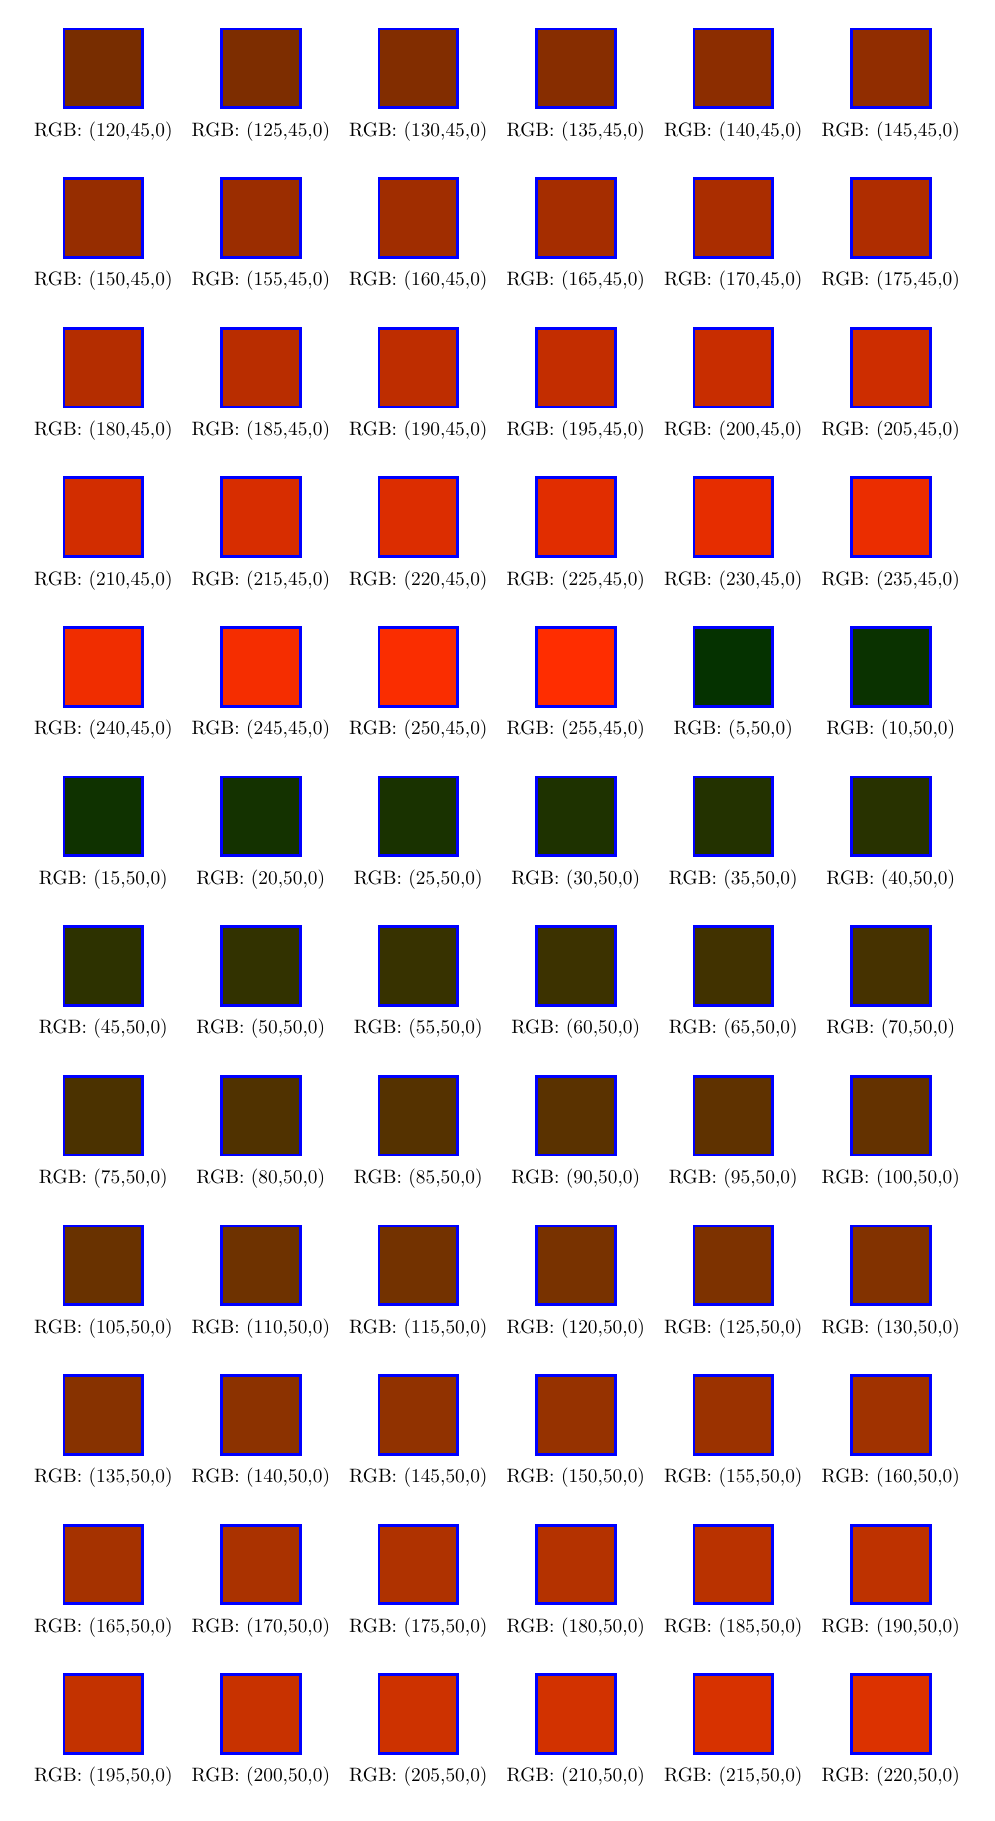
\begin{tikzpicture}

    \filldraw[draw=blue,line width=1,fill=colorR120G45B0]
    (0,0) rectangle (1,1);

    \node[scale=0.7] at (0.5,-0.3) {RGB: (120,45,0)};



    \begin{scope}[xshift=2cm]

      \filldraw[draw=blue,line width=1,fill=colorR125G45B0]
      (0,0) rectangle (1,1);

      \node[scale=0.7] at (0.5,-0.3) {RGB: (125,45,0)};

    \end{scope}



    \begin{scope}[xshift=4cm]

      \filldraw[draw=blue,line width=1,fill=colorR130G45B0]
      (0,0) rectangle (1,1);

      \node[scale=0.7] at (0.5,-0.3) {RGB: (130,45,0)};

    \end{scope}



    \begin{scope}[xshift=6cm]

      \filldraw[draw=blue,line width=1,fill=colorR135G45B0]
      (0,0) rectangle (1,1);

      \node[scale=0.7] at (0.5,-0.3) {RGB: (135,45,0)};

    \end{scope}



    \begin{scope}[xshift=8cm]

      \filldraw[draw=blue,line width=1,fill=colorR140G45B0]
      (0,0) rectangle (1,1);

      \node[scale=0.7] at (0.5,-0.3) {RGB: (140,45,0)};

    \end{scope}



    \begin{scope}[xshift=10cm]

      \filldraw[draw=blue,line width=1,fill=colorR145G45B0]
      (0,0) rectangle (1,1);

      \node[scale=0.7] at (0.5,-0.3) {RGB: (145,45,0)};

    \end{scope}







    \begin{scope}[yshift=-1.9cm]

      \filldraw[draw=blue,line width=1,fill=colorR150G45B0]
      (0,0) rectangle (1,1);

      \node[scale=0.7] at (0.5,-0.3) {RGB: (150,45,0)};

    \end{scope}



    \begin{scope}[xshift=2cm,yshift=-1.9cm]

      \filldraw[draw=blue,line width=1,fill=colorR155G45B0]
      (0,0) rectangle (1,1);

      \node[scale=0.7] at (0.5,-0.3) {RGB: (155,45,0)};

    \end{scope}



    \begin{scope}[xshift=4cm,yshift=-1.9cm]

      \filldraw[draw=blue,line width=1,fill=colorR160G45B0]
      (0,0) rectangle (1,1);

      \node[scale=0.7] at (0.5,-0.3) {RGB: (160,45,0)};

    \end{scope}



    \begin{scope}[xshift=6cm,yshift=-1.9cm]

      \filldraw[draw=blue,line width=1,fill=colorR165G45B0]
      (0,0) rectangle (1,1);

      \node[scale=0.7] at (0.5,-0.3) {RGB: (165,45,0)};

    \end{scope}



    \begin{scope}[xshift=8cm,yshift=-1.9cm]

      \filldraw[draw=blue,line width=1,fill=colorR170G45B0]
      (0,0) rectangle (1,1);

      \node[scale=0.7] at (0.5,-0.3) {RGB: (170,45,0)};

    \end{scope}



    \begin{scope}[xshift=10cm,yshift=-1.9cm]

      \filldraw[draw=blue,line width=1,fill=colorR175G45B0]
      (0,0) rectangle (1,1);

      \node[scale=0.7] at (0.5,-0.3) {RGB: (175,45,0)};

    \end{scope}







    \begin{scope}[yshift=-3.8cm]

      \filldraw[draw=blue,line width=1,fill=colorR180G45B0]
      (0,0) rectangle (1,1);

      \node[scale=0.7] at (0.5,-0.3) {RGB: (180,45,0)};

    \end{scope}



    \begin{scope}[xshift=2cm,yshift=-3.8cm]

      \filldraw[draw=blue,line width=1,fill=colorR185G45B0]
      (0,0) rectangle (1,1);

      \node[scale=0.7] at (0.5,-0.3) {RGB: (185,45,0)};

    \end{scope}



    \begin{scope}[xshift=4cm,yshift=-3.8cm]

      \filldraw[draw=blue,line width=1,fill=colorR190G45B0]
      (0,0) rectangle (1,1);

      \node[scale=0.7] at (0.5,-0.3) {RGB: (190,45,0)};

    \end{scope}



    \begin{scope}[xshift=6cm,yshift=-3.8cm]

      \filldraw[draw=blue,line width=1,fill=colorR195G45B0]
      (0,0) rectangle (1,1);

      \node[scale=0.7] at (0.5,-0.3) {RGB: (195,45,0)};

    \end{scope}



    \begin{scope}[xshift=8cm,yshift=-3.8cm]

      \filldraw[draw=blue,line width=1,fill=colorR200G45B0]
      (0,0) rectangle (1,1);

      \node[scale=0.7] at (0.5,-0.3) {RGB: (200,45,0)};

    \end{scope}



    \begin{scope}[xshift=10cm,yshift=-3.8cm]

      \filldraw[draw=blue,line width=1,fill=colorR205G45B0]
      (0,0) rectangle (1,1);

      \node[scale=0.7] at (0.5,-0.3) {RGB: (205,45,0)};

    \end{scope}







    \begin{scope}[yshift=-5.7cm]

      \filldraw[draw=blue,line width=1,fill=colorR210G45B0]
      (0,0) rectangle (1,1);

      \node[scale=0.7] at (0.5,-0.3) {RGB: (210,45,0)};

    \end{scope}



    \begin{scope}[xshift=2cm,yshift=-5.7cm]

      \filldraw[draw=blue,line width=1,fill=colorR215G45B0]
      (0,0) rectangle (1,1);

      \node[scale=0.7] at (0.5,-0.3) {RGB: (215,45,0)};

    \end{scope}



    \begin{scope}[xshift=4cm,yshift=-5.7cm]

      \filldraw[draw=blue,line width=1,fill=colorR220G45B0]
      (0,0) rectangle (1,1);

      \node[scale=0.7] at (0.5,-0.3) {RGB: (220,45,0)};

    \end{scope}



    \begin{scope}[xshift=6cm,yshift=-5.7cm]

      \filldraw[draw=blue,line width=1,fill=colorR225G45B0]
      (0,0) rectangle (1,1);

      \node[scale=0.7] at (0.5,-0.3) {RGB: (225,45,0)};

    \end{scope}



    \begin{scope}[xshift=8cm,yshift=-5.7cm]

      \filldraw[draw=blue,line width=1,fill=colorR230G45B0]
      (0,0) rectangle (1,1);

      \node[scale=0.7] at (0.5,-0.3) {RGB: (230,45,0)};

    \end{scope}



    \begin{scope}[xshift=10cm,yshift=-5.7cm]

      \filldraw[draw=blue,line width=1,fill=colorR235G45B0]
      (0,0) rectangle (1,1);

      \node[scale=0.7] at (0.5,-0.3) {RGB: (235,45,0)};

    \end{scope}







    \begin{scope}[yshift=-7.6cm]

      \filldraw[draw=blue,line width=1,fill=colorR240G45B0]
      (0,0) rectangle (1,1);

      \node[scale=0.7] at (0.5,-0.3) {RGB: (240,45,0)};

    \end{scope}



    \begin{scope}[xshift=2cm,yshift=-7.6cm]

      \filldraw[draw=blue,line width=1,fill=colorR245G45B0]
      (0,0) rectangle (1,1);

      \node[scale=0.7] at (0.5,-0.3) {RGB: (245,45,0)};

    \end{scope}



    \begin{scope}[xshift=4cm,yshift=-7.6cm]

      \filldraw[draw=blue,line width=1,fill=colorR250G45B0]
      (0,0) rectangle (1,1);

      \node[scale=0.7] at (0.5,-0.3) {RGB: (250,45,0)};

    \end{scope}



    \begin{scope}[xshift=6cm,yshift=-7.6cm]

      \filldraw[draw=blue,line width=1,fill=colorR255G45B0]
      (0,0) rectangle (1,1);

      \node[scale=0.7] at (0.5,-0.3) {RGB: (255,45,0)};

    \end{scope}



    \begin{scope}[xshift=8cm,yshift=-7.6cm]

      \filldraw[draw=blue,line width=1,fill=colorR5G50B0]
      (0,0) rectangle (1,1);

      \node[scale=0.7] at (0.5,-0.3) {RGB: (5,50,0)};

    \end{scope}



    \begin{scope}[xshift=10cm,yshift=-7.6cm]

      \filldraw[draw=blue,line width=1,fill=colorR10G50B0]
      (0,0) rectangle (1,1);

      \node[scale=0.7] at (0.5,-0.3) {RGB: (10,50,0)};

    \end{scope}







    \begin{scope}[yshift=-9.5cm]

      \filldraw[draw=blue,line width=1,fill=colorR15G50B0]
      (0,0) rectangle (1,1);

      \node[scale=0.7] at (0.5,-0.3) {RGB: (15,50,0)};

    \end{scope}



    \begin{scope}[xshift=2cm,yshift=-9.5cm]

      \filldraw[draw=blue,line width=1,fill=colorR20G50B0]
      (0,0) rectangle (1,1);

      \node[scale=0.7] at (0.5,-0.3) {RGB: (20,50,0)};

    \end{scope}



    \begin{scope}[xshift=4cm,yshift=-9.5cm]

      \filldraw[draw=blue,line width=1,fill=colorR25G50B0]
      (0,0) rectangle (1,1);

      \node[scale=0.7] at (0.5,-0.3) {RGB: (25,50,0)};

    \end{scope}



    \begin{scope}[xshift=6cm,yshift=-9.5cm]

      \filldraw[draw=blue,line width=1,fill=colorR30G50B0]
      (0,0) rectangle (1,1);

      \node[scale=0.7] at (0.5,-0.3) {RGB: (30,50,0)};

    \end{scope}



    \begin{scope}[xshift=8cm,yshift=-9.5cm]

      \filldraw[draw=blue,line width=1,fill=colorR35G50B0]
      (0,0) rectangle (1,1);

      \node[scale=0.7] at (0.5,-0.3) {RGB: (35,50,0)};

    \end{scope}



    \begin{scope}[xshift=10cm,yshift=-9.5cm]

      \filldraw[draw=blue,line width=1,fill=colorR40G50B0]
      (0,0) rectangle (1,1);

      \node[scale=0.7] at (0.5,-0.3) {RGB: (40,50,0)};

    \end{scope}







    \begin{scope}[yshift=-11.4cm]

      \filldraw[draw=blue,line width=1,fill=colorR45G50B0]
      (0,0) rectangle (1,1);

      \node[scale=0.7] at (0.5,-0.3) {RGB: (45,50,0)};

    \end{scope}



    \begin{scope}[xshift=2cm,yshift=-11.4cm]

      \filldraw[draw=blue,line width=1,fill=colorR50G50B0]
      (0,0) rectangle (1,1);

      \node[scale=0.7] at (0.5,-0.3) {RGB: (50,50,0)};

    \end{scope}



    \begin{scope}[xshift=4cm,yshift=-11.4cm]

      \filldraw[draw=blue,line width=1,fill=colorR55G50B0]
      (0,0) rectangle (1,1);

      \node[scale=0.7] at (0.5,-0.3) {RGB: (55,50,0)};

    \end{scope}



    \begin{scope}[xshift=6cm,yshift=-11.4cm]

      \filldraw[draw=blue,line width=1,fill=colorR60G50B0]
      (0,0) rectangle (1,1);

      \node[scale=0.7] at (0.5,-0.3) {RGB: (60,50,0)};

    \end{scope}



    \begin{scope}[xshift=8cm,yshift=-11.4cm]

      \filldraw[draw=blue,line width=1,fill=colorR65G50B0]
      (0,0) rectangle (1,1);

      \node[scale=0.7] at (0.5,-0.3) {RGB: (65,50,0)};

    \end{scope}



    \begin{scope}[xshift=10cm,yshift=-11.4cm]

      \filldraw[draw=blue,line width=1,fill=colorR70G50B0]
      (0,0) rectangle (1,1);

      \node[scale=0.7] at (0.5,-0.3) {RGB: (70,50,0)};

    \end{scope}







    \begin{scope}[yshift=-13.3cm]

      \filldraw[draw=blue,line width=1,fill=colorR75G50B0]
      (0,0) rectangle (1,1);

      \node[scale=0.7] at (0.5,-0.3) {RGB: (75,50,0)};

    \end{scope}



    \begin{scope}[xshift=2cm,yshift=-13.3cm]

      \filldraw[draw=blue,line width=1,fill=colorR80G50B0]
      (0,0) rectangle (1,1);

      \node[scale=0.7] at (0.5,-0.3) {RGB: (80,50,0)};

    \end{scope}



    \begin{scope}[xshift=4cm,yshift=-13.3cm]

      \filldraw[draw=blue,line width=1,fill=colorR85G50B0]
      (0,0) rectangle (1,1);

      \node[scale=0.7] at (0.5,-0.3) {RGB: (85,50,0)};

    \end{scope}



    \begin{scope}[xshift=6cm,yshift=-13.3cm]

      \filldraw[draw=blue,line width=1,fill=colorR90G50B0]
      (0,0) rectangle (1,1);

      \node[scale=0.7] at (0.5,-0.3) {RGB: (90,50,0)};

    \end{scope}



    \begin{scope}[xshift=8cm,yshift=-13.3cm]

      \filldraw[draw=blue,line width=1,fill=colorR95G50B0]
      (0,0) rectangle (1,1);

      \node[scale=0.7] at (0.5,-0.3) {RGB: (95,50,0)};

    \end{scope}



    \begin{scope}[xshift=10cm,yshift=-13.3cm]

      \filldraw[draw=blue,line width=1,fill=colorR100G50B0]
      (0,0) rectangle (1,1);

      \node[scale=0.7] at (0.5,-0.3) {RGB: (100,50,0)};

    \end{scope}







    \begin{scope}[yshift=-15.2cm]

      \filldraw[draw=blue,line width=1,fill=colorR105G50B0]
      (0,0) rectangle (1,1);

      \node[scale=0.7] at (0.5,-0.3) {RGB: (105,50,0)};

    \end{scope}



    \begin{scope}[xshift=2cm,yshift=-15.2cm]

      \filldraw[draw=blue,line width=1,fill=colorR110G50B0]
      (0,0) rectangle (1,1);

      \node[scale=0.7] at (0.5,-0.3) {RGB: (110,50,0)};

    \end{scope}



    \begin{scope}[xshift=4cm,yshift=-15.2cm]

      \filldraw[draw=blue,line width=1,fill=colorR115G50B0]
      (0,0) rectangle (1,1);

      \node[scale=0.7] at (0.5,-0.3) {RGB: (115,50,0)};

    \end{scope}



    \begin{scope}[xshift=6cm,yshift=-15.2cm]

      \filldraw[draw=blue,line width=1,fill=colorR120G50B0]
      (0,0) rectangle (1,1);

      \node[scale=0.7] at (0.5,-0.3) {RGB: (120,50,0)};

    \end{scope}



    \begin{scope}[xshift=8cm,yshift=-15.2cm]

      \filldraw[draw=blue,line width=1,fill=colorR125G50B0]
      (0,0) rectangle (1,1);

      \node[scale=0.7] at (0.5,-0.3) {RGB: (125,50,0)};

    \end{scope}



    \begin{scope}[xshift=10cm,yshift=-15.2cm]

      \filldraw[draw=blue,line width=1,fill=colorR130G50B0]
      (0,0) rectangle (1,1);

      \node[scale=0.7] at (0.5,-0.3) {RGB: (130,50,0)};

    \end{scope}







    \begin{scope}[yshift=-17.1cm]

      \filldraw[draw=blue,line width=1,fill=colorR135G50B0]
      (0,0) rectangle (1,1);

      \node[scale=0.7] at (0.5,-0.3) {RGB: (135,50,0)};

    \end{scope}



    \begin{scope}[xshift=2cm,yshift=-17.1cm]

      \filldraw[draw=blue,line width=1,fill=colorR140G50B0]
      (0,0) rectangle (1,1);

      \node[scale=0.7] at (0.5,-0.3) {RGB: (140,50,0)};

    \end{scope}



    \begin{scope}[xshift=4cm,yshift=-17.1cm]

      \filldraw[draw=blue,line width=1,fill=colorR145G50B0]
      (0,0) rectangle (1,1);

      \node[scale=0.7] at (0.5,-0.3) {RGB: (145,50,0)};

    \end{scope}



    \begin{scope}[xshift=6cm,yshift=-17.1cm]

      \filldraw[draw=blue,line width=1,fill=colorR150G50B0]
      (0,0) rectangle (1,1);

      \node[scale=0.7] at (0.5,-0.3) {RGB: (150,50,0)};

    \end{scope}



    \begin{scope}[xshift=8cm,yshift=-17.1cm]

      \filldraw[draw=blue,line width=1,fill=colorR155G50B0]
      (0,0) rectangle (1,1);

      \node[scale=0.7] at (0.5,-0.3) {RGB: (155,50,0)};

    \end{scope}



    \begin{scope}[xshift=10cm,yshift=-17.1cm]

      \filldraw[draw=blue,line width=1,fill=colorR160G50B0]
      (0,0) rectangle (1,1);

      \node[scale=0.7] at (0.5,-0.3) {RGB: (160,50,0)};

    \end{scope}







    \begin{scope}[yshift=-19cm]

      \filldraw[draw=blue,line width=1,fill=colorR165G50B0]
      (0,0) rectangle (1,1);

      \node[scale=0.7] at (0.5,-0.3) {RGB: (165,50,0)};

    \end{scope}



    \begin{scope}[xshift=2cm,yshift=-19cm]

      \filldraw[draw=blue,line width=1,fill=colorR170G50B0]
      (0,0) rectangle (1,1);

      \node[scale=0.7] at (0.5,-0.3) {RGB: (170,50,0)};

    \end{scope}



    \begin{scope}[xshift=4cm,yshift=-19cm]

      \filldraw[draw=blue,line width=1,fill=colorR175G50B0]
      (0,0) rectangle (1,1);

      \node[scale=0.7] at (0.5,-0.3) {RGB: (175,50,0)};

    \end{scope}



    \begin{scope}[xshift=6cm,yshift=-19cm]

      \filldraw[draw=blue,line width=1,fill=colorR180G50B0]
      (0,0) rectangle (1,1);

      \node[scale=0.7] at (0.5,-0.3) {RGB: (180,50,0)};

    \end{scope}



    \begin{scope}[xshift=8cm,yshift=-19cm]

      \filldraw[draw=blue,line width=1,fill=colorR185G50B0]
      (0,0) rectangle (1,1);

      \node[scale=0.7] at (0.5,-0.3) {RGB: (185,50,0)};

    \end{scope}



    \begin{scope}[xshift=10cm,yshift=-19cm]

      \filldraw[draw=blue,line width=1,fill=colorR190G50B0]
      (0,0) rectangle (1,1);

      \node[scale=0.7] at (0.5,-0.3) {RGB: (190,50,0)};

    \end{scope}







    \begin{scope}[yshift=-20.9cm]

      \filldraw[draw=blue,line width=1,fill=colorR195G50B0]
      (0,0) rectangle (1,1);

      \node[scale=0.7] at (0.5,-0.3) {RGB: (195,50,0)};

    \end{scope}



    \begin{scope}[xshift=2cm,yshift=-20.9cm]

      \filldraw[draw=blue,line width=1,fill=colorR200G50B0]
      (0,0) rectangle (1,1);

      \node[scale=0.7] at (0.5,-0.3) {RGB: (200,50,0)};

    \end{scope}



    \begin{scope}[xshift=4cm,yshift=-20.9cm]

      \filldraw[draw=blue,line width=1,fill=colorR205G50B0]
      (0,0) rectangle (1,1);

      \node[scale=0.7] at (0.5,-0.3) {RGB: (205,50,0)};

    \end{scope}



    \begin{scope}[xshift=6cm,yshift=-20.9cm]

      \filldraw[draw=blue,line width=1,fill=colorR210G50B0]
      (0,0) rectangle (1,1);

      \node[scale=0.7] at (0.5,-0.3) {RGB: (210,50,0)};

    \end{scope}



    \begin{scope}[xshift=8cm,yshift=-20.9cm]

      \filldraw[draw=blue,line width=1,fill=colorR215G50B0]
      (0,0) rectangle (1,1);

      \node[scale=0.7] at (0.5,-0.3) {RGB: (215,50,0)};

    \end{scope}



    \begin{scope}[xshift=10cm,yshift=-20.9cm]

      \filldraw[draw=blue,line width=1,fill=colorR220G50B0]
      (0,0) rectangle (1,1);

      \node[scale=0.7] at (0.5,-0.3) {RGB: (220,50,0)};

    \end{scope}

  \end{tikzpicture}

  \caption{Mixed colors in~RGB system: $(120,45,0)$--$(255,45,0)$,
    $(5,50,0)$--$(220,50,0)$}



  \label{fig:Mixed-colors-Part-07}

\end{figure}
% ##################





% ##################
\begin{figure}

  \centering


  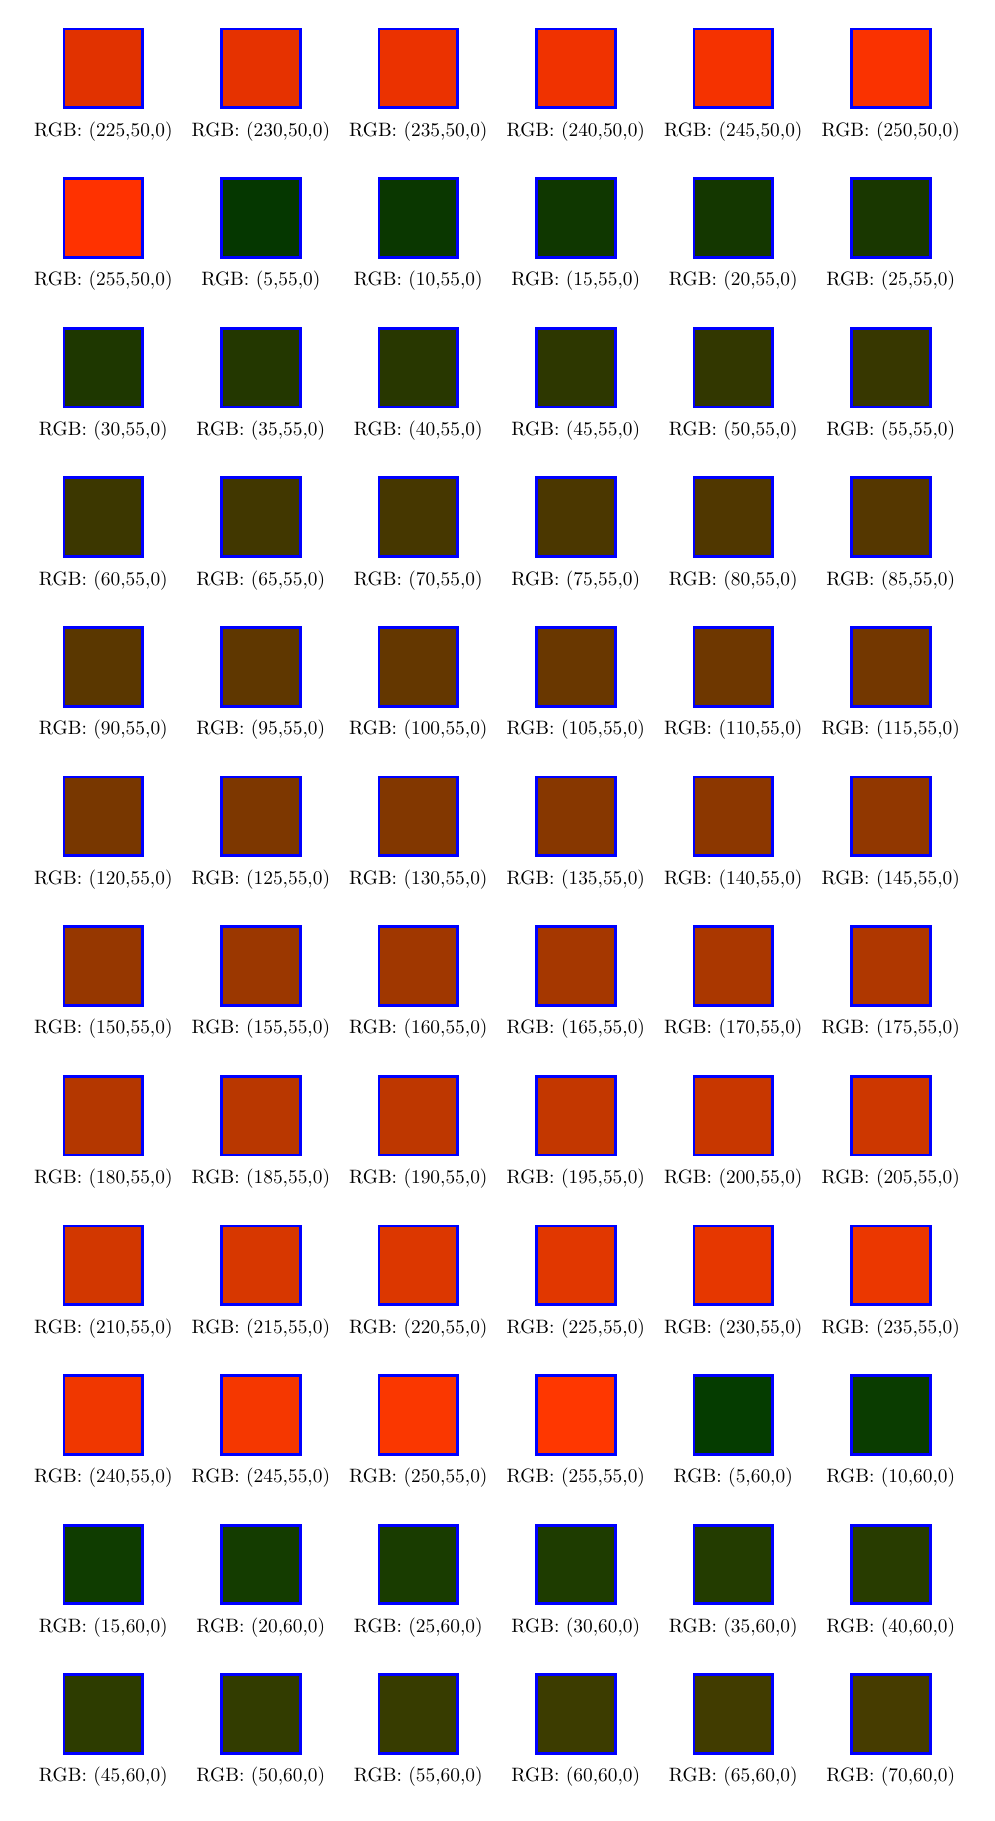
\begin{tikzpicture}

    \filldraw[draw=blue,line width=1,fill=colorR225G50B0]
    (0,0) rectangle (1,1);

    \node[scale=0.7] at (0.5,-0.3) {RGB: (225,50,0)};



    \begin{scope}[xshift=2cm]

      \filldraw[draw=blue,line width=1,fill=colorR230G50B0]
      (0,0) rectangle (1,1);

      \node[scale=0.7] at (0.5,-0.3) {RGB: (230,50,0)};

    \end{scope}



    \begin{scope}[xshift=4cm]

      \filldraw[draw=blue,line width=1,fill=colorR235G50B0]
      (0,0) rectangle (1,1);

      \node[scale=0.7] at (0.5,-0.3) {RGB: (235,50,0)};

    \end{scope}



    \begin{scope}[xshift=6cm]

      \filldraw[draw=blue,line width=1,fill=colorR240G50B0]
      (0,0) rectangle (1,1);

      \node[scale=0.7] at (0.5,-0.3) {RGB: (240,50,0)};

    \end{scope}



    \begin{scope}[xshift=8cm]

      \filldraw[draw=blue,line width=1,fill=colorR245G50B0]
      (0,0) rectangle (1,1);

      \node[scale=0.7] at (0.5,-0.3) {RGB: (245,50,0)};

    \end{scope}



    \begin{scope}[xshift=10cm]

      \filldraw[draw=blue,line width=1,fill=colorR250G50B0]
      (0,0) rectangle (1,1);

      \node[scale=0.7] at (0.5,-0.3) {RGB: (250,50,0)};

    \end{scope}







    \begin{scope}[yshift=-1.9cm]

      \filldraw[draw=blue,line width=1,fill=colorR255G50B0]
      (0,0) rectangle (1,1);

      \node[scale=0.7] at (0.5,-0.3) {RGB: (255,50,0)};

    \end{scope}



    \begin{scope}[xshift=2cm,yshift=-1.9cm]

      \filldraw[draw=blue,line width=1,fill=colorR5G55B0]
      (0,0) rectangle (1,1);

      \node[scale=0.7] at (0.5,-0.3) {RGB: (5,55,0)};

    \end{scope}



    \begin{scope}[xshift=4cm,yshift=-1.9cm]

      \filldraw[draw=blue,line width=1,fill=colorR10G55B0]
      (0,0) rectangle (1,1);

      \node[scale=0.7] at (0.5,-0.3) {RGB: (10,55,0)};

    \end{scope}



    \begin{scope}[xshift=6cm,yshift=-1.9cm]

      \filldraw[draw=blue,line width=1,fill=colorR15G55B0]
      (0,0) rectangle (1,1);

      \node[scale=0.7] at (0.5,-0.3) {RGB: (15,55,0)};

    \end{scope}



    \begin{scope}[xshift=8cm,yshift=-1.9cm]

      \filldraw[draw=blue,line width=1,fill=colorR20G55B0]
      (0,0) rectangle (1,1);

      \node[scale=0.7] at (0.5,-0.3) {RGB: (20,55,0)};

    \end{scope}



    \begin{scope}[xshift=10cm,yshift=-1.9cm]

      \filldraw[draw=blue,line width=1,fill=colorR25G55B0]
      (0,0) rectangle (1,1);

      \node[scale=0.7] at (0.5,-0.3) {RGB: (25,55,0)};

    \end{scope}







    \begin{scope}[yshift=-3.8cm]

      \filldraw[draw=blue,line width=1,fill=colorR30G55B0]
      (0,0) rectangle (1,1);

      \node[scale=0.7] at (0.5,-0.3) {RGB: (30,55,0)};

    \end{scope}



    \begin{scope}[xshift=2cm,yshift=-3.8cm]

      \filldraw[draw=blue,line width=1,fill=colorR35G55B0]
      (0,0) rectangle (1,1);

      \node[scale=0.7] at (0.5,-0.3) {RGB: (35,55,0)};

    \end{scope}



    \begin{scope}[xshift=4cm,yshift=-3.8cm]

      \filldraw[draw=blue,line width=1,fill=colorR40G55B0]
      (0,0) rectangle (1,1);

      \node[scale=0.7] at (0.5,-0.3) {RGB: (40,55,0)};

    \end{scope}



    \begin{scope}[xshift=6cm,yshift=-3.8cm]

      \filldraw[draw=blue,line width=1,fill=colorR45G55B0]
      (0,0) rectangle (1,1);

      \node[scale=0.7] at (0.5,-0.3) {RGB: (45,55,0)};

    \end{scope}



    \begin{scope}[xshift=8cm,yshift=-3.8cm]

      \filldraw[draw=blue,line width=1,fill=colorR50G55B0]
      (0,0) rectangle (1,1);

      \node[scale=0.7] at (0.5,-0.3) {RGB: (50,55,0)};

    \end{scope}



    \begin{scope}[xshift=10cm,yshift=-3.8cm]

      \filldraw[draw=blue,line width=1,fill=colorR55G55B0]
      (0,0) rectangle (1,1);

      \node[scale=0.7] at (0.5,-0.3) {RGB: (55,55,0)};

    \end{scope}







    \begin{scope}[yshift=-5.7cm]

      \filldraw[draw=blue,line width=1,fill=colorR60G55B0]
      (0,0) rectangle (1,1);

      \node[scale=0.7] at (0.5,-0.3) {RGB: (60,55,0)};

    \end{scope}



    \begin{scope}[xshift=2cm,yshift=-5.7cm]

      \filldraw[draw=blue,line width=1,fill=colorR65G55B0]
      (0,0) rectangle (1,1);

      \node[scale=0.7] at (0.5,-0.3) {RGB: (65,55,0)};

    \end{scope}



    \begin{scope}[xshift=4cm,yshift=-5.7cm]

      \filldraw[draw=blue,line width=1,fill=colorR70G55B0]
      (0,0) rectangle (1,1);

      \node[scale=0.7] at (0.5,-0.3) {RGB: (70,55,0)};

    \end{scope}



    \begin{scope}[xshift=6cm,yshift=-5.7cm]

      \filldraw[draw=blue,line width=1,fill=colorR75G55B0]
      (0,0) rectangle (1,1);

      \node[scale=0.7] at (0.5,-0.3) {RGB: (75,55,0)};

    \end{scope}



    \begin{scope}[xshift=8cm,yshift=-5.7cm]

      \filldraw[draw=blue,line width=1,fill=colorR80G55B0]
      (0,0) rectangle (1,1);

      \node[scale=0.7] at (0.5,-0.3) {RGB: (80,55,0)};

    \end{scope}



    \begin{scope}[xshift=10cm,yshift=-5.7cm]

      \filldraw[draw=blue,line width=1,fill=colorR85G55B0]
      (0,0) rectangle (1,1);

      \node[scale=0.7] at (0.5,-0.3) {RGB: (85,55,0)};

    \end{scope}







    \begin{scope}[yshift=-7.6cm]

      \filldraw[draw=blue,line width=1,fill=colorR90G55B0]
      (0,0) rectangle (1,1);

      \node[scale=0.7] at (0.5,-0.3) {RGB: (90,55,0)};

    \end{scope}



    \begin{scope}[xshift=2cm,yshift=-7.6cm]

      \filldraw[draw=blue,line width=1,fill=colorR95G55B0]
      (0,0) rectangle (1,1);

      \node[scale=0.7] at (0.5,-0.3) {RGB: (95,55,0)};

    \end{scope}



    \begin{scope}[xshift=4cm,yshift=-7.6cm]

      \filldraw[draw=blue,line width=1,fill=colorR100G55B0]
      (0,0) rectangle (1,1);

      \node[scale=0.7] at (0.5,-0.3) {RGB: (100,55,0)};

    \end{scope}



    \begin{scope}[xshift=6cm,yshift=-7.6cm]

      \filldraw[draw=blue,line width=1,fill=colorR105G55B0]
      (0,0) rectangle (1,1);

      \node[scale=0.7] at (0.5,-0.3) {RGB: (105,55,0)};

    \end{scope}



    \begin{scope}[xshift=8cm,yshift=-7.6cm]

      \filldraw[draw=blue,line width=1,fill=colorR110G55B0]
      (0,0) rectangle (1,1);

      \node[scale=0.7] at (0.5,-0.3) {RGB: (110,55,0)};

    \end{scope}



    \begin{scope}[xshift=10cm,yshift=-7.6cm]

      \filldraw[draw=blue,line width=1,fill=colorR115G55B0]
      (0,0) rectangle (1,1);

      \node[scale=0.7] at (0.5,-0.3) {RGB: (115,55,0)};

    \end{scope}







    \begin{scope}[yshift=-9.5cm]

      \filldraw[draw=blue,line width=1,fill=colorR120G55B0]
      (0,0) rectangle (1,1);

      \node[scale=0.7] at (0.5,-0.3) {RGB: (120,55,0)};

    \end{scope}



    \begin{scope}[xshift=2cm,yshift=-9.5cm]

      \filldraw[draw=blue,line width=1,fill=colorR125G55B0]
      (0,0) rectangle (1,1);

      \node[scale=0.7] at (0.5,-0.3) {RGB: (125,55,0)};

    \end{scope}



    \begin{scope}[xshift=4cm,yshift=-9.5cm]

      \filldraw[draw=blue,line width=1,fill=colorR130G55B0]
      (0,0) rectangle (1,1);

      \node[scale=0.7] at (0.5,-0.3) {RGB: (130,55,0)};

    \end{scope}



    \begin{scope}[xshift=6cm,yshift=-9.5cm]

      \filldraw[draw=blue,line width=1,fill=colorR135G55B0]
      (0,0) rectangle (1,1);

      \node[scale=0.7] at (0.5,-0.3) {RGB: (135,55,0)};

    \end{scope}



    \begin{scope}[xshift=8cm,yshift=-9.5cm]

      \filldraw[draw=blue,line width=1,fill=colorR140G55B0]
      (0,0) rectangle (1,1);

      \node[scale=0.7] at (0.5,-0.3) {RGB: (140,55,0)};

    \end{scope}



    \begin{scope}[xshift=10cm,yshift=-9.5cm]

      \filldraw[draw=blue,line width=1,fill=colorR145G55B0]
      (0,0) rectangle (1,1);

      \node[scale=0.7] at (0.5,-0.3) {RGB: (145,55,0)};

    \end{scope}







    \begin{scope}[yshift=-11.4cm]

      \filldraw[draw=blue,line width=1,fill=colorR150G55B0]
      (0,0) rectangle (1,1);

      \node[scale=0.7] at (0.5,-0.3) {RGB: (150,55,0)};

    \end{scope}



    \begin{scope}[xshift=2cm,yshift=-11.4cm]

      \filldraw[draw=blue,line width=1,fill=colorR155G55B0]
      (0,0) rectangle (1,1);

      \node[scale=0.7] at (0.5,-0.3) {RGB: (155,55,0)};

    \end{scope}



    \begin{scope}[xshift=4cm,yshift=-11.4cm]

      \filldraw[draw=blue,line width=1,fill=colorR160G55B0]
      (0,0) rectangle (1,1);

      \node[scale=0.7] at (0.5,-0.3) {RGB: (160,55,0)};

    \end{scope}



    \begin{scope}[xshift=6cm,yshift=-11.4cm]

      \filldraw[draw=blue,line width=1,fill=colorR165G55B0]
      (0,0) rectangle (1,1);

      \node[scale=0.7] at (0.5,-0.3) {RGB: (165,55,0)};

    \end{scope}



    \begin{scope}[xshift=8cm,yshift=-11.4cm]

      \filldraw[draw=blue,line width=1,fill=colorR170G55B0]
      (0,0) rectangle (1,1);

      \node[scale=0.7] at (0.5,-0.3) {RGB: (170,55,0)};

    \end{scope}



    \begin{scope}[xshift=10cm,yshift=-11.4cm]

      \filldraw[draw=blue,line width=1,fill=colorR175G55B0]
      (0,0) rectangle (1,1);

      \node[scale=0.7] at (0.5,-0.3) {RGB: (175,55,0)};

    \end{scope}







    \begin{scope}[yshift=-13.3cm]

      \filldraw[draw=blue,line width=1,fill=colorR180G55B0]
      (0,0) rectangle (1,1);

      \node[scale=0.7] at (0.5,-0.3) {RGB: (180,55,0)};

    \end{scope}



    \begin{scope}[xshift=2cm,yshift=-13.3cm]

      \filldraw[draw=blue,line width=1,fill=colorR185G55B0]
      (0,0) rectangle (1,1);

      \node[scale=0.7] at (0.5,-0.3) {RGB: (185,55,0)};

    \end{scope}



    \begin{scope}[xshift=4cm,yshift=-13.3cm]

      \filldraw[draw=blue,line width=1,fill=colorR190G55B0]
      (0,0) rectangle (1,1);

      \node[scale=0.7] at (0.5,-0.3) {RGB: (190,55,0)};

    \end{scope}



    \begin{scope}[xshift=6cm,yshift=-13.3cm]

      \filldraw[draw=blue,line width=1,fill=colorR195G55B0]
      (0,0) rectangle (1,1);

      \node[scale=0.7] at (0.5,-0.3) {RGB: (195,55,0)};

    \end{scope}



    \begin{scope}[xshift=8cm,yshift=-13.3cm]

      \filldraw[draw=blue,line width=1,fill=colorR200G55B0]
      (0,0) rectangle (1,1);

      \node[scale=0.7] at (0.5,-0.3) {RGB: (200,55,0)};

    \end{scope}



    \begin{scope}[xshift=10cm,yshift=-13.3cm]

      \filldraw[draw=blue,line width=1,fill=colorR205G55B0]
      (0,0) rectangle (1,1);

      \node[scale=0.7] at (0.5,-0.3) {RGB: (205,55,0)};

    \end{scope}







    \begin{scope}[yshift=-15.2cm]

      \filldraw[draw=blue,line width=1,fill=colorR210G55B0]
      (0,0) rectangle (1,1);

      \node[scale=0.7] at (0.5,-0.3) {RGB: (210,55,0)};

    \end{scope}



    \begin{scope}[xshift=2cm,yshift=-15.2cm]

      \filldraw[draw=blue,line width=1,fill=colorR215G55B0]
      (0,0) rectangle (1,1);

      \node[scale=0.7] at (0.5,-0.3) {RGB: (215,55,0)};

    \end{scope}



    \begin{scope}[xshift=4cm,yshift=-15.2cm]

      \filldraw[draw=blue,line width=1,fill=colorR220G55B0]
      (0,0) rectangle (1,1);

      \node[scale=0.7] at (0.5,-0.3) {RGB: (220,55,0)};

    \end{scope}



    \begin{scope}[xshift=6cm,yshift=-15.2cm]

      \filldraw[draw=blue,line width=1,fill=colorR225G55B0]
      (0,0) rectangle (1,1);

      \node[scale=0.7] at (0.5,-0.3) {RGB: (225,55,0)};

    \end{scope}



    \begin{scope}[xshift=8cm,yshift=-15.2cm]

      \filldraw[draw=blue,line width=1,fill=colorR230G55B0]
      (0,0) rectangle (1,1);

      \node[scale=0.7] at (0.5,-0.3) {RGB: (230,55,0)};

    \end{scope}



    \begin{scope}[xshift=10cm,yshift=-15.2cm]

      \filldraw[draw=blue,line width=1,fill=colorR235G55B0]
      (0,0) rectangle (1,1);

      \node[scale=0.7] at (0.5,-0.3) {RGB: (235,55,0)};

    \end{scope}







    \begin{scope}[yshift=-17.1cm]

      \filldraw[draw=blue,line width=1,fill=colorR240G55B0]
      (0,0) rectangle (1,1);

      \node[scale=0.7] at (0.5,-0.3) {RGB: (240,55,0)};

    \end{scope}



    \begin{scope}[xshift=2cm,yshift=-17.1cm]

      \filldraw[draw=blue,line width=1,fill=colorR245G55B0]
      (0,0) rectangle (1,1);

      \node[scale=0.7] at (0.5,-0.3) {RGB: (245,55,0)};

    \end{scope}



    \begin{scope}[xshift=4cm,yshift=-17.1cm]

      \filldraw[draw=blue,line width=1,fill=colorR250G55B0]
      (0,0) rectangle (1,1);

      \node[scale=0.7] at (0.5,-0.3) {RGB: (250,55,0)};

    \end{scope}



    \begin{scope}[xshift=6cm,yshift=-17.1cm]

      \filldraw[draw=blue,line width=1,fill=colorR255G55B0]
      (0,0) rectangle (1,1);

      \node[scale=0.7] at (0.5,-0.3) {RGB: (255,55,0)};

    \end{scope}



    \begin{scope}[xshift=8cm,yshift=-17.1cm]

      \filldraw[draw=blue,line width=1,fill=colorR5G60B0]
      (0,0) rectangle (1,1);

      \node[scale=0.7] at (0.5,-0.3) {RGB: (5,60,0)};

    \end{scope}



    \begin{scope}[xshift=10cm,yshift=-17.1cm]

      \filldraw[draw=blue,line width=1,fill=colorR10G60B0]
      (0,0) rectangle (1,1);

      \node[scale=0.7] at (0.5,-0.3) {RGB: (10,60,0)};

    \end{scope}







    \begin{scope}[yshift=-19cm]

      \filldraw[draw=blue,line width=1,fill=colorR15G60B0]
      (0,0) rectangle (1,1);

      \node[scale=0.7] at (0.5,-0.3) {RGB: (15,60,0)};

    \end{scope}



    \begin{scope}[xshift=2cm,yshift=-19cm]

      \filldraw[draw=blue,line width=1,fill=colorR20G60B0]
      (0,0) rectangle (1,1);

      \node[scale=0.7] at (0.5,-0.3) {RGB: (20,60,0)};

    \end{scope}



    \begin{scope}[xshift=4cm,yshift=-19cm]

      \filldraw[draw=blue,line width=1,fill=colorR25G60B0]
      (0,0) rectangle (1,1);

      \node[scale=0.7] at (0.5,-0.3) {RGB: (25,60,0)};

    \end{scope}



    \begin{scope}[xshift=6cm,yshift=-19cm]

      \filldraw[draw=blue,line width=1,fill=colorR30G60B0]
      (0,0) rectangle (1,1);

      \node[scale=0.7] at (0.5,-0.3) {RGB: (30,60,0)};

    \end{scope}



    \begin{scope}[xshift=8cm,yshift=-19cm]

      \filldraw[draw=blue,line width=1,fill=colorR35G60B0]
      (0,0) rectangle (1,1);

      \node[scale=0.7] at (0.5,-0.3) {RGB: (35,60,0)};

    \end{scope}



    \begin{scope}[xshift=10cm,yshift=-19cm]

      \filldraw[draw=blue,line width=1,fill=colorR40G60B0]
      (0,0) rectangle (1,1);

      \node[scale=0.7] at (0.5,-0.3) {RGB: (40,60,0)};

    \end{scope}







    \begin{scope}[yshift=-20.9cm]

      \filldraw[draw=blue,line width=1,fill=colorR45G60B0]
      (0,0) rectangle (1,1);

      \node[scale=0.7] at (0.5,-0.3) {RGB: (45,60,0)};

    \end{scope}



    \begin{scope}[xshift=2cm,yshift=-20.9cm]

      \filldraw[draw=blue,line width=1,fill=colorR50G60B0]
      (0,0) rectangle (1,1);

      \node[scale=0.7] at (0.5,-0.3) {RGB: (50,60,0)};

    \end{scope}



    \begin{scope}[xshift=4cm,yshift=-20.9cm]

      \filldraw[draw=blue,line width=1,fill=colorR55G60B0]
      (0,0) rectangle (1,1);

      \node[scale=0.7] at (0.5,-0.3) {RGB: (55,60,0)};

    \end{scope}



    \begin{scope}[xshift=6cm,yshift=-20.9cm]

      \filldraw[draw=blue,line width=1,fill=colorR60G60B0]
      (0,0) rectangle (1,1);

      \node[scale=0.7] at (0.5,-0.3) {RGB: (60,60,0)};

    \end{scope}



    \begin{scope}[xshift=8cm,yshift=-20.9cm]

      \filldraw[draw=blue,line width=1,fill=colorR65G60B0]
      (0,0) rectangle (1,1);

      \node[scale=0.7] at (0.5,-0.3) {RGB: (65,60,0)};

    \end{scope}



    \begin{scope}[xshift=10cm,yshift=-20.9cm]

      \filldraw[draw=blue,line width=1,fill=colorR70G60B0]
      (0,0) rectangle (1,1);

      \node[scale=0.7] at (0.5,-0.3) {RGB: (70,60,0)};

    \end{scope}

  \end{tikzpicture}

  \caption{Mixed colors in~RGB system: $(225,50,0)$--$(255,50,0)$,
    $(5,55,0)$--$(255,55,0)$, $(5,60,0)$--$(70,60,0)$}



  \label{fig:Mixed-colors-Part-08}

\end{figure}
% ##################





% ##################
\begin{figure}

  \centering


  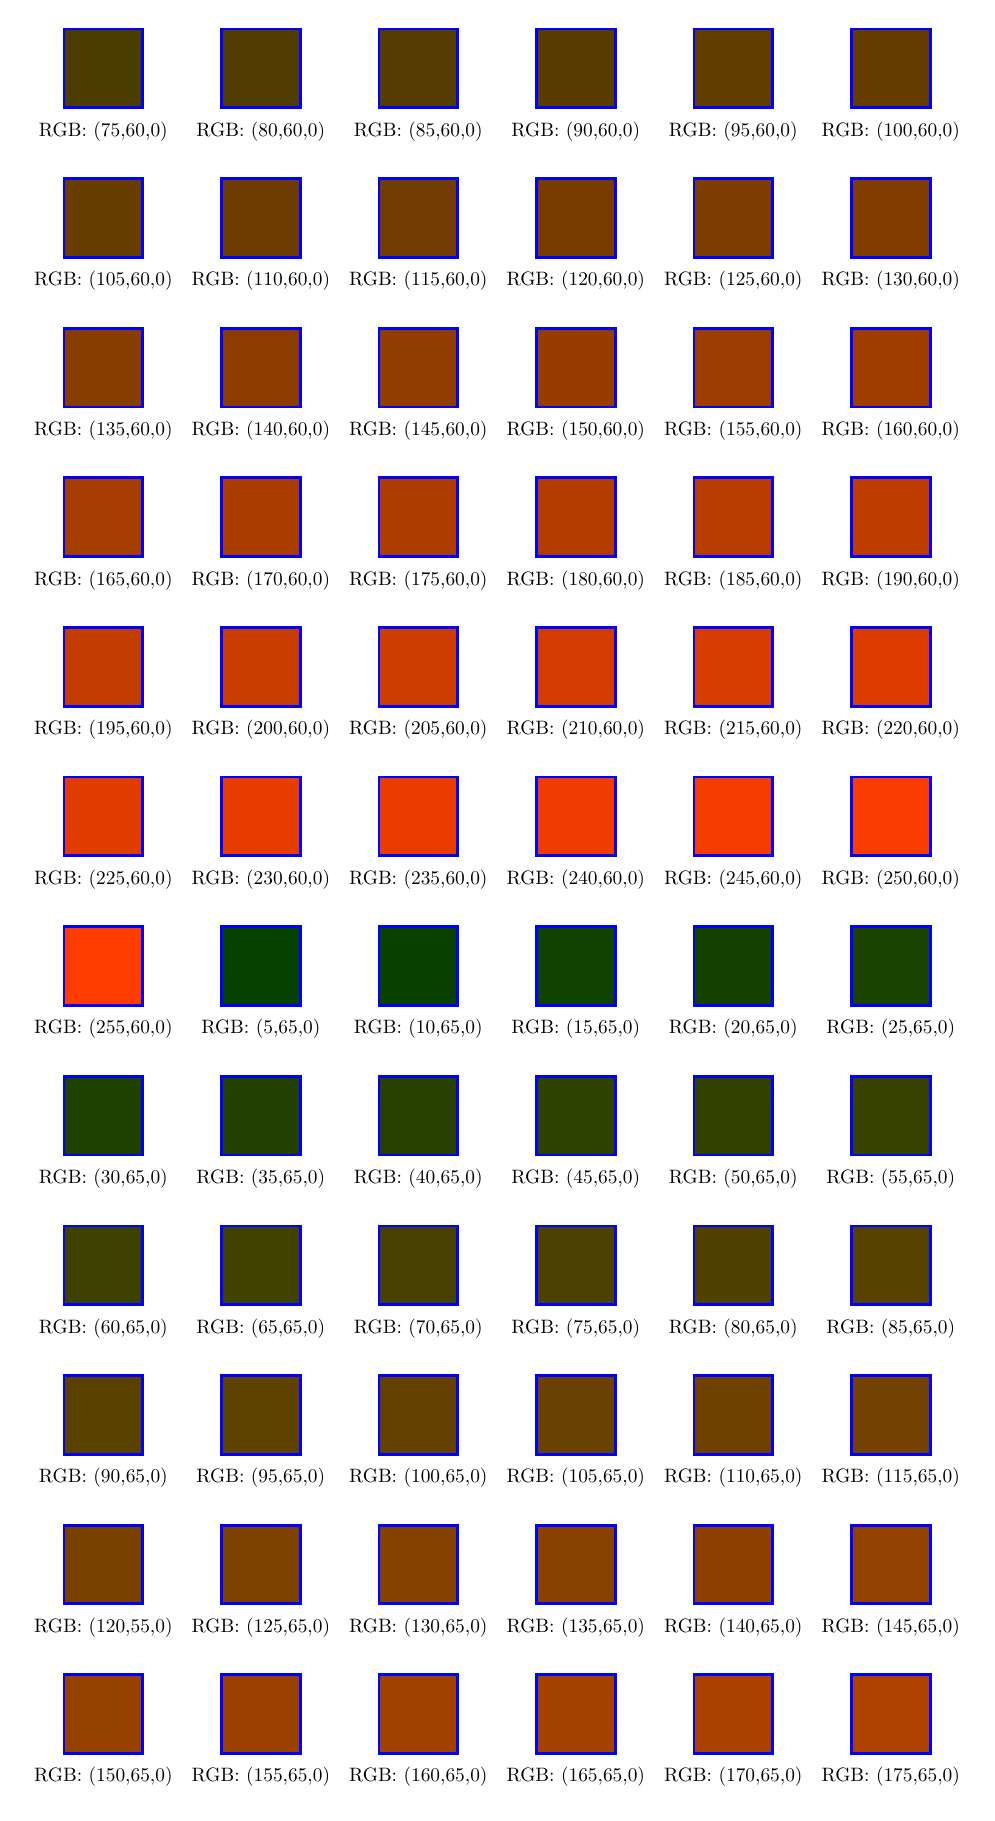
\begin{tikzpicture}

    \filldraw[draw=blue,line width=1,fill=colorR75G60B0]
    (0,0) rectangle (1,1);

    \node[scale=0.7] at (0.5,-0.3) {RGB: (75,60,0)};



    \begin{scope}[xshift=2cm]

      \filldraw[draw=blue,line width=1,fill=colorR80G60B0]
      (0,0) rectangle (1,1);

      \node[scale=0.7] at (0.5,-0.3) {RGB: (80,60,0)};

    \end{scope}



    \begin{scope}[xshift=4cm]

      \filldraw[draw=blue,line width=1,fill=colorR85G60B0]
      (0,0) rectangle (1,1);

      \node[scale=0.7] at (0.5,-0.3) {RGB: (85,60,0)};

    \end{scope}



    \begin{scope}[xshift=6cm]

      \filldraw[draw=blue,line width=1,fill=colorR90G60B0]
      (0,0) rectangle (1,1);

      \node[scale=0.7] at (0.5,-0.3) {RGB: (90,60,0)};

    \end{scope}



    \begin{scope}[xshift=8cm]

      \filldraw[draw=blue,line width=1,fill=colorR95G60B0]
      (0,0) rectangle (1,1);

      \node[scale=0.7] at (0.5,-0.3) {RGB: (95,60,0)};

    \end{scope}



    \begin{scope}[xshift=10cm]

      \filldraw[draw=blue,line width=1,fill=colorR100G60B0]
      (0,0) rectangle (1,1);

      \node[scale=0.7] at (0.5,-0.3) {RGB: (100,60,0)};

    \end{scope}







    \begin{scope}[yshift=-1.9cm]

      \filldraw[draw=blue,line width=1,fill=colorR105G60B0]
      (0,0) rectangle (1,1);

      \node[scale=0.7] at (0.5,-0.3) {RGB: (105,60,0)};

    \end{scope}



    \begin{scope}[xshift=2cm,yshift=-1.9cm]

      \filldraw[draw=blue,line width=1,fill=colorR110G60B0]
      (0,0) rectangle (1,1);

      \node[scale=0.7] at (0.5,-0.3) {RGB: (110,60,0)};

    \end{scope}



    \begin{scope}[xshift=4cm,yshift=-1.9cm]

      \filldraw[draw=blue,line width=1,fill=colorR115G60B0]
      (0,0) rectangle (1,1);

      \node[scale=0.7] at (0.5,-0.3) {RGB: (115,60,0)};

    \end{scope}



    \begin{scope}[xshift=6cm,yshift=-1.9cm]

      \filldraw[draw=blue,line width=1,fill=colorR120G60B0]
      (0,0) rectangle (1,1);

      \node[scale=0.7] at (0.5,-0.3) {RGB: (120,60,0)};

    \end{scope}



    \begin{scope}[xshift=8cm,yshift=-1.9cm]

      \filldraw[draw=blue,line width=1,fill=colorR125G60B0]
      (0,0) rectangle (1,1);

      \node[scale=0.7] at (0.5,-0.3) {RGB: (125,60,0)};

    \end{scope}



    \begin{scope}[xshift=10cm,yshift=-1.9cm]

      \filldraw[draw=blue,line width=1,fill=colorR130G60B0]
      (0,0) rectangle (1,1);

      \node[scale=0.7] at (0.5,-0.3) {RGB: (130,60,0)};

    \end{scope}







    \begin{scope}[yshift=-3.8cm]

      \filldraw[draw=blue,line width=1,fill=colorR135G60B0]
      (0,0) rectangle (1,1);

      \node[scale=0.7] at (0.5,-0.3) {RGB: (135,60,0)};

    \end{scope}



    \begin{scope}[xshift=2cm,yshift=-3.8cm]

      \filldraw[draw=blue,line width=1,fill=colorR140G60B0]
      (0,0) rectangle (1,1);

      \node[scale=0.7] at (0.5,-0.3) {RGB: (140,60,0)};

    \end{scope}



    \begin{scope}[xshift=4cm,yshift=-3.8cm]

      \filldraw[draw=blue,line width=1,fill=colorR145G60B0]
      (0,0) rectangle (1,1);

      \node[scale=0.7] at (0.5,-0.3) {RGB: (145,60,0)};

    \end{scope}



    \begin{scope}[xshift=6cm,yshift=-3.8cm]

      \filldraw[draw=blue,line width=1,fill=colorR150G60B0]
      (0,0) rectangle (1,1);

      \node[scale=0.7] at (0.5,-0.3) {RGB: (150,60,0)};

    \end{scope}



    \begin{scope}[xshift=8cm,yshift=-3.8cm]

      \filldraw[draw=blue,line width=1,fill=colorR155G60B0]
      (0,0) rectangle (1,1);

      \node[scale=0.7] at (0.5,-0.3) {RGB: (155,60,0)};

    \end{scope}



    \begin{scope}[xshift=10cm,yshift=-3.8cm]

      \filldraw[draw=blue,line width=1,fill=colorR160G60B0]
      (0,0) rectangle (1,1);

      \node[scale=0.7] at (0.5,-0.3) {RGB: (160,60,0)};

    \end{scope}







    \begin{scope}[yshift=-5.7cm]

      \filldraw[draw=blue,line width=1,fill=colorR165G60B0]
      (0,0) rectangle (1,1);

      \node[scale=0.7] at (0.5,-0.3) {RGB: (165,60,0)};

    \end{scope}



    \begin{scope}[xshift=2cm,yshift=-5.7cm]

      \filldraw[draw=blue,line width=1,fill=colorR170G60B0]
      (0,0) rectangle (1,1);

      \node[scale=0.7] at (0.5,-0.3) {RGB: (170,60,0)};

    \end{scope}



    \begin{scope}[xshift=4cm,yshift=-5.7cm]

      \filldraw[draw=blue,line width=1,fill=colorR175G60B0]
      (0,0) rectangle (1,1);

      \node[scale=0.7] at (0.5,-0.3) {RGB: (175,60,0)};

    \end{scope}



    \begin{scope}[xshift=6cm,yshift=-5.7cm]

      \filldraw[draw=blue,line width=1,fill=colorR180G60B0]
      (0,0) rectangle (1,1);

      \node[scale=0.7] at (0.5,-0.3) {RGB: (180,60,0)};

    \end{scope}



    \begin{scope}[xshift=8cm,yshift=-5.7cm]

      \filldraw[draw=blue,line width=1,fill=colorR185G60B0]
      (0,0) rectangle (1,1);

      \node[scale=0.7] at (0.5,-0.3) {RGB: (185,60,0)};

    \end{scope}



    \begin{scope}[xshift=10cm,yshift=-5.7cm]

      \filldraw[draw=blue,line width=1,fill=colorR190G60B0]
      (0,0) rectangle (1,1);

      \node[scale=0.7] at (0.5,-0.3) {RGB: (190,60,0)};

    \end{scope}







    \begin{scope}[yshift=-7.6cm]

      \filldraw[draw=blue,line width=1,fill=colorR195G60B0]
      (0,0) rectangle (1,1);

      \node[scale=0.7] at (0.5,-0.3) {RGB: (195,60,0)};

    \end{scope}



    \begin{scope}[xshift=2cm,yshift=-7.6cm]

      \filldraw[draw=blue,line width=1,fill=colorR200G60B0]
      (0,0) rectangle (1,1);

      \node[scale=0.7] at (0.5,-0.3) {RGB: (200,60,0)};

    \end{scope}



    \begin{scope}[xshift=4cm,yshift=-7.6cm]

      \filldraw[draw=blue,line width=1,fill=colorR205G60B0]
      (0,0) rectangle (1,1);

      \node[scale=0.7] at (0.5,-0.3) {RGB: (205,60,0)};

    \end{scope}



    \begin{scope}[xshift=6cm,yshift=-7.6cm]

      \filldraw[draw=blue,line width=1,fill=colorR210G60B0]
      (0,0) rectangle (1,1);

      \node[scale=0.7] at (0.5,-0.3) {RGB: (210,60,0)};

    \end{scope}



    \begin{scope}[xshift=8cm,yshift=-7.6cm]

      \filldraw[draw=blue,line width=1,fill=colorR215G60B0]
      (0,0) rectangle (1,1);

      \node[scale=0.7] at (0.5,-0.3) {RGB: (215,60,0)};

    \end{scope}



    \begin{scope}[xshift=10cm,yshift=-7.6cm]

      \filldraw[draw=blue,line width=1,fill=colorR220G60B0]
      (0,0) rectangle (1,1);

      \node[scale=0.7] at (0.5,-0.3) {RGB: (220,60,0)};

    \end{scope}







    \begin{scope}[yshift=-9.5cm]

      \filldraw[draw=blue,line width=1,fill=colorR225G60B0]
      (0,0) rectangle (1,1);

      \node[scale=0.7] at (0.5,-0.3) {RGB: (225,60,0)};

    \end{scope}



    \begin{scope}[xshift=2cm,yshift=-9.5cm]

      \filldraw[draw=blue,line width=1,fill=colorR230G60B0]
      (0,0) rectangle (1,1);

      \node[scale=0.7] at (0.5,-0.3) {RGB: (230,60,0)};

    \end{scope}



    \begin{scope}[xshift=4cm,yshift=-9.5cm]

      \filldraw[draw=blue,line width=1,fill=colorR235G60B0]
      (0,0) rectangle (1,1);

      \node[scale=0.7] at (0.5,-0.3) {RGB: (235,60,0)};

    \end{scope}



    \begin{scope}[xshift=6cm,yshift=-9.5cm]

      \filldraw[draw=blue,line width=1,fill=colorR240G60B0]
      (0,0) rectangle (1,1);

      \node[scale=0.7] at (0.5,-0.3) {RGB: (240,60,0)};

    \end{scope}



    \begin{scope}[xshift=8cm,yshift=-9.5cm]

      \filldraw[draw=blue,line width=1,fill=colorR245G60B0]
      (0,0) rectangle (1,1);

      \node[scale=0.7] at (0.5,-0.3) {RGB: (245,60,0)};

    \end{scope}



    \begin{scope}[xshift=10cm,yshift=-9.5cm]

      \filldraw[draw=blue,line width=1,fill=colorR250G60B0]
      (0,0) rectangle (1,1);

      \node[scale=0.7] at (0.5,-0.3) {RGB: (250,60,0)};

    \end{scope}







    \begin{scope}[yshift=-11.4cm]

      \filldraw[draw=blue,line width=1,fill=colorR255G60B0]
      (0,0) rectangle (1,1);

      \node[scale=0.7] at (0.5,-0.3) {RGB: (255,60,0)};

    \end{scope}



    \begin{scope}[xshift=2cm,yshift=-11.4cm]

      \filldraw[draw=blue,line width=1,fill=colorR5G65B0]
      (0,0) rectangle (1,1);

      \node[scale=0.7] at (0.5,-0.3) {RGB: (5,65,0)};

    \end{scope}



    \begin{scope}[xshift=4cm,yshift=-11.4cm]

      \filldraw[draw=blue,line width=1,fill=colorR10G65B0]
      (0,0) rectangle (1,1);

      \node[scale=0.7] at (0.5,-0.3) {RGB: (10,65,0)};

    \end{scope}



    \begin{scope}[xshift=6cm,yshift=-11.4cm]

      \filldraw[draw=blue,line width=1,fill=colorR15G65B0]
      (0,0) rectangle (1,1);

      \node[scale=0.7] at (0.5,-0.3) {RGB: (15,65,0)};

    \end{scope}



    \begin{scope}[xshift=8cm,yshift=-11.4cm]

      \filldraw[draw=blue,line width=1,fill=colorR20G65B0]
      (0,0) rectangle (1,1);

      \node[scale=0.7] at (0.5,-0.3) {RGB: (20,65,0)};

    \end{scope}



    \begin{scope}[xshift=10cm,yshift=-11.4cm]

      \filldraw[draw=blue,line width=1,fill=colorR25G65B0]
      (0,0) rectangle (1,1);

      \node[scale=0.7] at (0.5,-0.3) {RGB: (25,65,0)};

    \end{scope}







    \begin{scope}[yshift=-13.3cm]

      \filldraw[draw=blue,line width=1,fill=colorR30G65B0]
      (0,0) rectangle (1,1);

      \node[scale=0.7] at (0.5,-0.3) {RGB: (30,65,0)};

    \end{scope}



    \begin{scope}[xshift=2cm,yshift=-13.3cm]

      \filldraw[draw=blue,line width=1,fill=colorR35G65B0]
      (0,0) rectangle (1,1);

      \node[scale=0.7] at (0.5,-0.3) {RGB: (35,65,0)};

    \end{scope}



    \begin{scope}[xshift=4cm,yshift=-13.3cm]

      \filldraw[draw=blue,line width=1,fill=colorR40G65B0]
      (0,0) rectangle (1,1);

      \node[scale=0.7] at (0.5,-0.3) {RGB: (40,65,0)};

    \end{scope}



    \begin{scope}[xshift=6cm,yshift=-13.3cm]

      \filldraw[draw=blue,line width=1,fill=colorR45G65B0]
      (0,0) rectangle (1,1);

      \node[scale=0.7] at (0.5,-0.3) {RGB: (45,65,0)};

    \end{scope}



    \begin{scope}[xshift=8cm,yshift=-13.3cm]

      \filldraw[draw=blue,line width=1,fill=colorR50G65B0]
      (0,0) rectangle (1,1);

      \node[scale=0.7] at (0.5,-0.3) {RGB: (50,65,0)};

    \end{scope}



    \begin{scope}[xshift=10cm,yshift=-13.3cm]

      \filldraw[draw=blue,line width=1,fill=colorR55G65B0]
      (0,0) rectangle (1,1);

      \node[scale=0.7] at (0.5,-0.3) {RGB: (55,65,0)};

    \end{scope}







    \begin{scope}[yshift=-15.2cm]

      \filldraw[draw=blue,line width=1,fill=colorR60G65B0]
      (0,0) rectangle (1,1);

      \node[scale=0.7] at (0.5,-0.3) {RGB: (60,65,0)};

    \end{scope}



    \begin{scope}[xshift=2cm,yshift=-15.2cm]

      \filldraw[draw=blue,line width=1,fill=colorR65G65B0]
      (0,0) rectangle (1,1);

      \node[scale=0.7] at (0.5,-0.3) {RGB: (65,65,0)};

    \end{scope}



    \begin{scope}[xshift=4cm,yshift=-15.2cm]

      \filldraw[draw=blue,line width=1,fill=colorR70G65B0]
      (0,0) rectangle (1,1);

      \node[scale=0.7] at (0.5,-0.3) {RGB: (70,65,0)};

    \end{scope}



    \begin{scope}[xshift=6cm,yshift=-15.2cm]

      \filldraw[draw=blue,line width=1,fill=colorR75G65B0]
      (0,0) rectangle (1,1);

      \node[scale=0.7] at (0.5,-0.3) {RGB: (75,65,0)};

    \end{scope}



    \begin{scope}[xshift=8cm,yshift=-15.2cm]

      \filldraw[draw=blue,line width=1,fill=colorR80G65B0]
      (0,0) rectangle (1,1);

      \node[scale=0.7] at (0.5,-0.3) {RGB: (80,65,0)};

    \end{scope}



    \begin{scope}[xshift=10cm,yshift=-15.2cm]

      \filldraw[draw=blue,line width=1,fill=colorR85G65B0]
      (0,0) rectangle (1,1);

      \node[scale=0.7] at (0.5,-0.3) {RGB: (85,65,0)};

    \end{scope}







    \begin{scope}[yshift=-17.1cm]

      \filldraw[draw=blue,line width=1,fill=colorR90G65B0]
      (0,0) rectangle (1,1);

      \node[scale=0.7] at (0.5,-0.3) {RGB: (90,65,0)};

    \end{scope}



    \begin{scope}[xshift=2cm,yshift=-17.1cm]

      \filldraw[draw=blue,line width=1,fill=colorR95G65B0]
      (0,0) rectangle (1,1);

      \node[scale=0.7] at (0.5,-0.3) {RGB: (95,65,0)};

    \end{scope}



    \begin{scope}[xshift=4cm,yshift=-17.1cm]

      \filldraw[draw=blue,line width=1,fill=colorR100G65B0]
      (0,0) rectangle (1,1);

      \node[scale=0.7] at (0.5,-0.3) {RGB: (100,65,0)};

    \end{scope}



    \begin{scope}[xshift=6cm,yshift=-17.1cm]

      \filldraw[draw=blue,line width=1,fill=colorR105G65B0]
      (0,0) rectangle (1,1);

      \node[scale=0.7] at (0.5,-0.3) {RGB: (105,65,0)};

    \end{scope}



    \begin{scope}[xshift=8cm,yshift=-17.1cm]

      \filldraw[draw=blue,line width=1,fill=colorR110G65B0]
      (0,0) rectangle (1,1);

      \node[scale=0.7] at (0.5,-0.3) {RGB: (110,65,0)};

    \end{scope}



    \begin{scope}[xshift=10cm,yshift=-17.1cm]

      \filldraw[draw=blue,line width=1,fill=colorR115G65B0]
      (0,0) rectangle (1,1);

      \node[scale=0.7] at (0.5,-0.3) {RGB: (115,65,0)};

    \end{scope}







    \begin{scope}[yshift=-19cm]

      \filldraw[draw=blue,line width=1,fill=colorR120G65B0]
      (0,0) rectangle (1,1);

      \node[scale=0.7] at (0.5,-0.3) {RGB: (120,55,0)};

    \end{scope}



    \begin{scope}[xshift=2cm,yshift=-19cm]

      \filldraw[draw=blue,line width=1,fill=colorR125G65B0]
      (0,0) rectangle (1,1);

      \node[scale=0.7] at (0.5,-0.3) {RGB: (125,65,0)};

    \end{scope}



    \begin{scope}[xshift=4cm,yshift=-19cm]

      \filldraw[draw=blue,line width=1,fill=colorR130G65B0]
      (0,0) rectangle (1,1);

      \node[scale=0.7] at (0.5,-0.3) {RGB: (130,65,0)};

    \end{scope}



    \begin{scope}[xshift=6cm,yshift=-19cm]

      \filldraw[draw=blue,line width=1,fill=colorR135G65B0]
      (0,0) rectangle (1,1);

      \node[scale=0.7] at (0.5,-0.3) {RGB: (135,65,0)};

    \end{scope}



    \begin{scope}[xshift=8cm,yshift=-19cm]

      \filldraw[draw=blue,line width=1,fill=colorR140G65B0]
      (0,0) rectangle (1,1);

      \node[scale=0.7] at (0.5,-0.3) {RGB: (140,65,0)};

    \end{scope}



    \begin{scope}[xshift=10cm,yshift=-19cm]

      \filldraw[draw=blue,line width=1,fill=colorR145G65B0]
      (0,0) rectangle (1,1);

      \node[scale=0.7] at (0.5,-0.3) {RGB: (145,65,0)};

    \end{scope}







    \begin{scope}[yshift=-20.9cm]

      \filldraw[draw=blue,line width=1,fill=colorR150G65B0]
      (0,0) rectangle (1,1);

      \node[scale=0.7] at (0.5,-0.3) {RGB: (150,65,0)};

    \end{scope}



    \begin{scope}[xshift=2cm,yshift=-20.9cm]

      \filldraw[draw=blue,line width=1,fill=colorR155G65B0]
      (0,0) rectangle (1,1);

      \node[scale=0.7] at (0.5,-0.3) {RGB: (155,65,0)};

    \end{scope}



    \begin{scope}[xshift=4cm,yshift=-20.9cm]

      \filldraw[draw=blue,line width=1,fill=colorR160G65B0]
      (0,0) rectangle (1,1);

      \node[scale=0.7] at (0.5,-0.3) {RGB: (160,65,0)};

    \end{scope}



    \begin{scope}[xshift=6cm,yshift=-20.9cm]

      \filldraw[draw=blue,line width=1,fill=colorR165G65B0]
      (0,0) rectangle (1,1);

      \node[scale=0.7] at (0.5,-0.3) {RGB: (165,65,0)};

    \end{scope}



    \begin{scope}[xshift=8cm,yshift=-20.9cm]

      \filldraw[draw=blue,line width=1,fill=colorR170G65B0]
      (0,0) rectangle (1,1);

      \node[scale=0.7] at (0.5,-0.3) {RGB: (170,65,0)};

    \end{scope}



    \begin{scope}[xshift=10cm,yshift=-20.9cm]

      \filldraw[draw=blue,line width=1,fill=colorR175G65B0]
      (0,0) rectangle (1,1);

      \node[scale=0.7] at (0.5,-0.3) {RGB: (175,65,0)};

    \end{scope}

  \end{tikzpicture}

  \caption{Mixed colors in~RGB system: $(75,60,0)$--$(255,60,0)$,
    $(5,65,0)$--$(175,65,0)$}



  \label{fig:Mixed-colors-Part-09}

\end{figure}
% ##################





% ##################
\begin{figure}

  \centering


  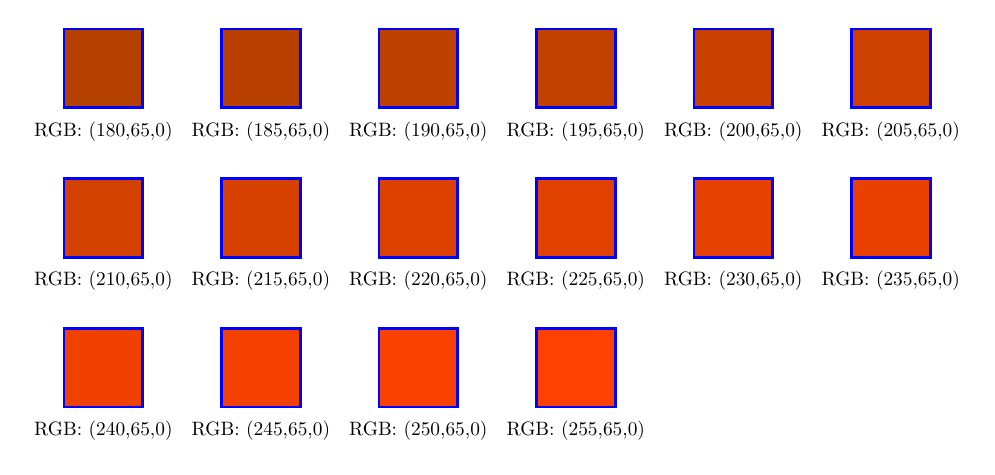
\begin{tikzpicture}

    \filldraw[draw=blue,line width=1,fill=colorR180G65B0]
    (0,0) rectangle (1,1);

    \node[scale=0.7] at (0.5,-0.3) {RGB: (180,65,0)};



    \begin{scope}[xshift=2cm]

      \filldraw[draw=blue,line width=1,fill=colorR185G65B0]
      (0,0) rectangle (1,1);

      \node[scale=0.7] at (0.5,-0.3) {RGB: (185,65,0)};

    \end{scope}



    \begin{scope}[xshift=4cm]

      \filldraw[draw=blue,line width=1,fill=colorR190G65B0]
      (0,0) rectangle (1,1);

      \node[scale=0.7] at (0.5,-0.3) {RGB: (190,65,0)};

    \end{scope}



    \begin{scope}[xshift=6cm]

      \filldraw[draw=blue,line width=1,fill=colorR195G65B0]
      (0,0) rectangle (1,1);

      \node[scale=0.7] at (0.5,-0.3) {RGB: (195,65,0)};

    \end{scope}



    \begin{scope}[xshift=8cm]

      \filldraw[draw=blue,line width=1,fill=colorR200G65B0]
      (0,0) rectangle (1,1);

      \node[scale=0.7] at (0.5,-0.3) {RGB: (200,65,0)};

    \end{scope}



    \begin{scope}[xshift=10cm]

      \filldraw[draw=blue,line width=1,fill=colorR205G65B0]
      (0,0) rectangle (1,1);

      \node[scale=0.7] at (0.5,-0.3) {RGB: (205,65,0)};

    \end{scope}







    \begin{scope}[yshift=-1.9cm]

      \filldraw[draw=blue,line width=1,fill=colorR210G65B0]
      (0,0) rectangle (1,1);

      \node[scale=0.7] at (0.5,-0.3) {RGB: (210,65,0)};

    \end{scope}



    \begin{scope}[xshift=2cm,yshift=-1.9cm]

      \filldraw[draw=blue,line width=1,fill=colorR215G65B0]
      (0,0) rectangle (1,1);

      \node[scale=0.7] at (0.5,-0.3) {RGB: (215,65,0)};

    \end{scope}



    \begin{scope}[xshift=4cm,yshift=-1.9cm]

      \filldraw[draw=blue,line width=1,fill=colorR220G65B0]
      (0,0) rectangle (1,1);

      \node[scale=0.7] at (0.5,-0.3) {RGB: (220,65,0)};

    \end{scope}



    \begin{scope}[xshift=6cm,yshift=-1.9cm]

      \filldraw[draw=blue,line width=1,fill=colorR225G65B0]
      (0,0) rectangle (1,1);

      \node[scale=0.7] at (0.5,-0.3) {RGB: (225,65,0)};

    \end{scope}



    \begin{scope}[xshift=8cm,yshift=-1.9cm]

      \filldraw[draw=blue,line width=1,fill=colorR230G65B0]
      (0,0) rectangle (1,1);

      \node[scale=0.7] at (0.5,-0.3) {RGB: (230,65,0)};

    \end{scope}



    \begin{scope}[xshift=10cm,yshift=-1.9cm]

      \filldraw[draw=blue,line width=1,fill=colorR235G65B0]
      (0,0) rectangle (1,1);

      \node[scale=0.7] at (0.5,-0.3) {RGB: (235,65,0)};

    \end{scope}







    \begin{scope}[yshift=-3.8cm]

      \filldraw[draw=blue,line width=1,fill=colorR240G65B0]
      (0,0) rectangle (1,1);

      \node[scale=0.7] at (0.5,-0.3) {RGB: (240,65,0)};

    \end{scope}



    \begin{scope}[xshift=2cm,yshift=-3.8cm]

      \filldraw[draw=blue,line width=1,fill=colorR245G65B0]
      (0,0) rectangle (1,1);

      \node[scale=0.7] at (0.5,-0.3) {RGB: (245,65,0)};

    \end{scope}



    \begin{scope}[xshift=4cm,yshift=-3.8cm]

      \filldraw[draw=blue,line width=1,fill=colorR250G65B0]
      (0,0) rectangle (1,1);

      \node[scale=0.7] at (0.5,-0.3) {RGB: (250,65,0)};

    \end{scope}



    \begin{scope}[xshift=6cm,yshift=-3.8cm]

      \filldraw[draw=blue,line width=1,fill=colorR255G65B0]
      (0,0) rectangle (1,1);

      \node[scale=0.7] at (0.5,-0.3) {RGB: (255,65,0)};

    \end{scope}



    % \begin{scope}[xshift=8cm,yshift=-1.9cm]

    %   \filldraw[draw=blue,line width=1,fill=colorR230G65B0]
    %   (0,0) rectangle (1,1);

    %   \node[scale=0.7] at (0.5,-0.3) {RGB: (230,65,0)};

    % \end{scope}



    % \begin{scope}[xshift=10cm,yshift=-1.9cm]

    %   \filldraw[draw=blue,line width=1,fill=colorR235G65B0]
    %   (0,0) rectangle (1,1);

    %   \node[scale=0.7] at (0.5,-0.3) {RGB: (235,65,0)};

    % \end{scope}

  \end{tikzpicture}

  \caption{Mixed colors in~RGB system: $(180,65,0)$--$(255,65,0)$}



  \label{fig:Mixed-colors-Part-10}

\end{figure}
% ##################










% ####################################################################
% ####################################################################
% Bibliography

% \printbibliography





% ############################
% End of the document

\end{document}
